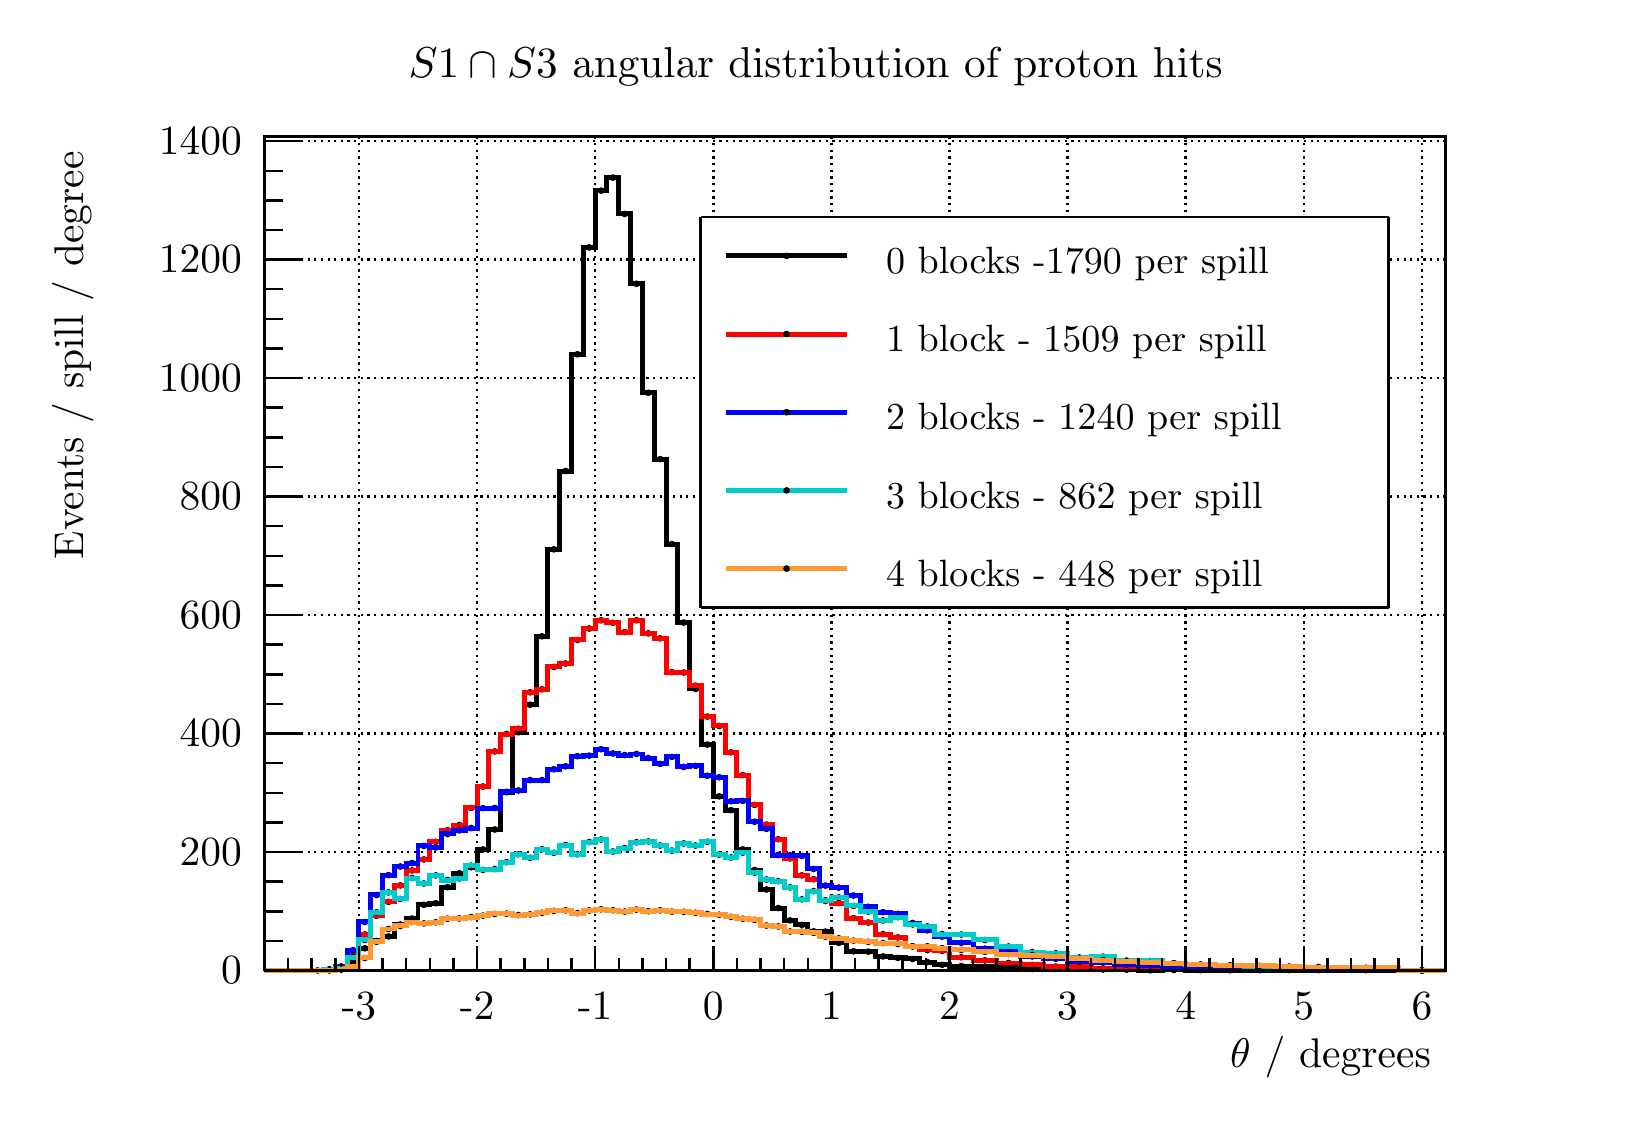
\begin{tikzpicture}
\pgfdeclareplotmark{cross} {
\pgfpathmoveto{\pgfpoint{-0.3\pgfplotmarksize}{\pgfplotmarksize}}
\pgfpathlineto{\pgfpoint{+0.3\pgfplotmarksize}{\pgfplotmarksize}}
\pgfpathlineto{\pgfpoint{+0.3\pgfplotmarksize}{0.3\pgfplotmarksize}}
\pgfpathlineto{\pgfpoint{+1\pgfplotmarksize}{0.3\pgfplotmarksize}}
\pgfpathlineto{\pgfpoint{+1\pgfplotmarksize}{-0.3\pgfplotmarksize}}
\pgfpathlineto{\pgfpoint{+0.3\pgfplotmarksize}{-0.3\pgfplotmarksize}}
\pgfpathlineto{\pgfpoint{+0.3\pgfplotmarksize}{-1.\pgfplotmarksize}}
\pgfpathlineto{\pgfpoint{-0.3\pgfplotmarksize}{-1.\pgfplotmarksize}}
\pgfpathlineto{\pgfpoint{-0.3\pgfplotmarksize}{-0.3\pgfplotmarksize}}
\pgfpathlineto{\pgfpoint{-1.\pgfplotmarksize}{-0.3\pgfplotmarksize}}
\pgfpathlineto{\pgfpoint{-1.\pgfplotmarksize}{0.3\pgfplotmarksize}}
\pgfpathlineto{\pgfpoint{-0.3\pgfplotmarksize}{0.3\pgfplotmarksize}}
\pgfpathclose
\pgfusepathqstroke
}
\pgfdeclareplotmark{cross*} {
\pgfpathmoveto{\pgfpoint{-0.3\pgfplotmarksize}{\pgfplotmarksize}}
\pgfpathlineto{\pgfpoint{+0.3\pgfplotmarksize}{\pgfplotmarksize}}
\pgfpathlineto{\pgfpoint{+0.3\pgfplotmarksize}{0.3\pgfplotmarksize}}
\pgfpathlineto{\pgfpoint{+1\pgfplotmarksize}{0.3\pgfplotmarksize}}
\pgfpathlineto{\pgfpoint{+1\pgfplotmarksize}{-0.3\pgfplotmarksize}}
\pgfpathlineto{\pgfpoint{+0.3\pgfplotmarksize}{-0.3\pgfplotmarksize}}
\pgfpathlineto{\pgfpoint{+0.3\pgfplotmarksize}{-1.\pgfplotmarksize}}
\pgfpathlineto{\pgfpoint{-0.3\pgfplotmarksize}{-1.\pgfplotmarksize}}
\pgfpathlineto{\pgfpoint{-0.3\pgfplotmarksize}{-0.3\pgfplotmarksize}}
\pgfpathlineto{\pgfpoint{-1.\pgfplotmarksize}{-0.3\pgfplotmarksize}}
\pgfpathlineto{\pgfpoint{-1.\pgfplotmarksize}{0.3\pgfplotmarksize}}
\pgfpathlineto{\pgfpoint{-0.3\pgfplotmarksize}{0.3\pgfplotmarksize}}
\pgfpathclose
\pgfusepathqfillstroke
}
\pgfdeclareplotmark{newstar} {
\pgfpathmoveto{\pgfqpoint{0pt}{\pgfplotmarksize}}
\pgfpathlineto{\pgfqpointpolar{44}{0.5\pgfplotmarksize}}
\pgfpathlineto{\pgfqpointpolar{18}{\pgfplotmarksize}}
\pgfpathlineto{\pgfqpointpolar{-20}{0.5\pgfplotmarksize}}
\pgfpathlineto{\pgfqpointpolar{-54}{\pgfplotmarksize}}
\pgfpathlineto{\pgfqpointpolar{-90}{0.5\pgfplotmarksize}}
\pgfpathlineto{\pgfqpointpolar{234}{\pgfplotmarksize}}
\pgfpathlineto{\pgfqpointpolar{198}{0.5\pgfplotmarksize}}
\pgfpathlineto{\pgfqpointpolar{162}{\pgfplotmarksize}}
\pgfpathlineto{\pgfqpointpolar{134}{0.5\pgfplotmarksize}}
\pgfpathclose
\pgfusepathqstroke
}
\pgfdeclareplotmark{newstar*} {
\pgfpathmoveto{\pgfqpoint{0pt}{\pgfplotmarksize}}
\pgfpathlineto{\pgfqpointpolar{44}{0.5\pgfplotmarksize}}
\pgfpathlineto{\pgfqpointpolar{18}{\pgfplotmarksize}}
\pgfpathlineto{\pgfqpointpolar{-20}{0.5\pgfplotmarksize}}
\pgfpathlineto{\pgfqpointpolar{-54}{\pgfplotmarksize}}
\pgfpathlineto{\pgfqpointpolar{-90}{0.5\pgfplotmarksize}}
\pgfpathlineto{\pgfqpointpolar{234}{\pgfplotmarksize}}
\pgfpathlineto{\pgfqpointpolar{198}{0.5\pgfplotmarksize}}
\pgfpathlineto{\pgfqpointpolar{162}{\pgfplotmarksize}}
\pgfpathlineto{\pgfqpointpolar{134}{0.5\pgfplotmarksize}}
\pgfpathclose
\pgfusepathqfillstroke
}
\definecolor{c}{rgb}{1,1,1};
\draw [color=c, fill=c] (0,0) rectangle (20,13.7553);
\draw [color=c, fill=c] (3,1.78819) rectangle (18,12.3797);
\definecolor{c}{rgb}{0,0,0};
\draw [c,line width=0.9] (3,1.78819) -- (3,12.3797) -- (18,12.3797) -- (18,1.78819) -- (3,1.78819);
\definecolor{c}{rgb}{1,1,1};
\draw [color=c, fill=c] (3,1.78819) rectangle (18,12.3797);
\definecolor{c}{rgb}{0,0,0};
\draw [c,line width=0.9] (3,1.78819) -- (3,12.3797) -- (18,12.3797) -- (18,1.78819) -- (3,1.78819);
\draw [c,line width=0.9] (3,1.78819) -- (18,1.78819);
\draw [c,dash pattern=on 0.80pt off 1.60pt ,line width=0.9] (4.2,12.3797) -- (4.2,1.78819);
\draw [c,dash pattern=on 0.80pt off 1.60pt ,line width=0.9] (5.7,12.3797) -- (5.7,1.78819);
\draw [c,dash pattern=on 0.80pt off 1.60pt ,line width=0.9] (7.2,12.3797) -- (7.2,1.78819);
\draw [c,dash pattern=on 0.80pt off 1.60pt ,line width=0.9] (8.7,12.3797) -- (8.7,1.78819);
\draw [c,dash pattern=on 0.80pt off 1.60pt ,line width=0.9] (10.2,12.3797) -- (10.2,1.78819);
\draw [c,dash pattern=on 0.80pt off 1.60pt ,line width=0.9] (11.7,12.3797) -- (11.7,1.78819);
\draw [c,dash pattern=on 0.80pt off 1.60pt ,line width=0.9] (13.2,12.3797) -- (13.2,1.78819);
\draw [c,dash pattern=on 0.80pt off 1.60pt ,line width=0.9] (14.7,12.3797) -- (14.7,1.78819);
\draw [c,dash pattern=on 0.80pt off 1.60pt ,line width=0.9] (16.2,12.3797) -- (16.2,1.78819);
\draw [c,dash pattern=on 0.80pt off 1.60pt ,line width=0.9] (17.7,12.3797) -- (17.7,1.78819);
\draw [c,dash pattern=on 0.80pt off 1.60pt ,line width=0.9] (4.2,12.3797) -- (4.2,1.78819);
\draw [c,dash pattern=on 0.80pt off 1.60pt ,line width=0.9] (17.7,12.3797) -- (17.7,1.78819);
\draw [c,line width=0.9] (3,1.78819) -- (3,12.3797);
\draw [c,dash pattern=on 0.80pt off 1.60pt ,line width=0.9] (18,1.78819) -- (3,1.78819);
\draw [c,dash pattern=on 0.80pt off 1.60pt ,line width=0.9] (18,3.29291) -- (3,3.29291);
\draw [c,dash pattern=on 0.80pt off 1.60pt ,line width=0.9] (18,4.79763) -- (3,4.79763);
\draw [c,dash pattern=on 0.80pt off 1.60pt ,line width=0.9] (18,6.30235) -- (3,6.30235);
\draw [c,dash pattern=on 0.80pt off 1.60pt ,line width=0.9] (18,7.80708) -- (3,7.80708);
\draw [c,dash pattern=on 0.80pt off 1.60pt ,line width=0.9] (18,9.3118) -- (3,9.3118);
\draw [c,dash pattern=on 0.80pt off 1.60pt ,line width=0.9] (18,10.8165) -- (3,10.8165);
\draw [c,dash pattern=on 0.80pt off 1.60pt ,line width=0.9] (18,12.3212) -- (3,12.3212);
\draw [c,dash pattern=on 0.80pt off 1.60pt ,line width=0.9] (18,12.3212) -- (3,12.3212);
\definecolor{c}{rgb}{0,0,0.6};
\draw [c,line width=0.9] (3,1.78819) -- (3.15,1.78819) -- (3.15,1.78819) -- (3.3,1.78819) -- (3.3,1.78819) -- (3.45,1.78819) -- (3.45,1.78819) -- (3.6,1.78819) -- (3.6,1.78819) -- (3.75,1.78819) -- (3.75,1.78819) -- (3.9,1.78819) -- (3.9,1.78819) --
 (4.05,1.78819) -- (4.05,1.78819) -- (4.2,1.78819) -- (4.2,1.78819) -- (4.35,1.78819) -- (4.35,1.78819) -- (4.5,1.78819) -- (4.5,1.78819) -- (4.65,1.78819) -- (4.65,1.78819) -- (4.8,1.78819) -- (4.8,1.78819) -- (4.95,1.78819) -- (4.95,1.78819) --
 (5.1,1.78819) -- (5.1,1.78819) -- (5.25,1.78819) -- (5.25,1.78819) -- (5.4,1.78819) -- (5.4,1.78819) -- (5.55,1.78819) -- (5.55,1.78819) -- (5.7,1.78819) -- (5.7,1.78819) -- (5.85,1.78819) -- (5.85,1.78819) -- (6,1.78819) -- (6,1.78819) --
 (6.15,1.78819) -- (6.15,1.78819) -- (6.3,1.78819) -- (6.3,1.78819) -- (6.45,1.78819) -- (6.45,1.78819) -- (6.6,1.78819) -- (6.6,1.78819) -- (6.75,1.78819) -- (6.75,1.78819) -- (6.9,1.78819) -- (6.9,1.78819) -- (7.05,1.78819) -- (7.05,1.78819) --
 (7.2,1.78819) -- (7.2,1.78819) -- (7.35,1.78819) -- (7.35,1.78819) -- (7.5,1.78819) -- (7.5,1.78819) -- (7.65,1.78819) -- (7.65,1.78819) -- (7.8,1.78819) -- (7.8,1.78819) -- (7.95,1.78819) -- (7.95,1.78819) -- (8.1,1.78819) -- (8.1,1.78819) --
 (8.25,1.78819) -- (8.25,1.78819) -- (8.4,1.78819) -- (8.4,1.78819) -- (8.55,1.78819) -- (8.55,1.78819) -- (8.7,1.78819) -- (8.7,1.78819) -- (8.85,1.78819) -- (8.85,1.78819) -- (9,1.78819) -- (9,1.78819) -- (9.15,1.78819) -- (9.15,1.78819) --
 (9.3,1.78819) -- (9.3,1.78819) -- (9.45,1.78819) -- (9.45,1.78819) -- (9.6,1.78819) -- (9.6,1.78819) -- (9.75,1.78819) -- (9.75,1.78819) -- (9.9,1.78819) -- (9.9,1.78819) -- (10.05,1.78819) -- (10.05,1.78819) -- (10.2,1.78819) -- (10.2,1.78819) --
 (10.3875,1.78819) -- (10.3875,1.78819) -- (10.575,1.78819) -- (10.575,1.78819) -- (10.7625,1.78819) -- (10.7625,1.78819) -- (10.95,1.78819) -- (10.95,1.78819) -- (11.1375,1.78819) -- (11.1375,1.78819) -- (11.325,1.78819) -- (11.325,1.78819) --
 (11.5125,1.78819) -- (11.5125,1.78819) -- (11.7,1.78819) -- (11.7,1.78819) -- (12,1.78819) -- (12,1.78819) -- (12.3,1.78819) -- (12.3,1.78819) -- (12.6,1.78819) -- (12.6,1.78819) -- (12.9,1.78819) -- (12.9,1.78819) -- (13.2,1.78819) --
 (13.2,1.78819) -- (13.5,1.78819) -- (13.5,1.78819) -- (13.8,1.78819) -- (13.8,1.78819) -- (14.1,1.78819) -- (14.1,1.78819) -- (14.4,1.78819) -- (14.4,1.78819) -- (14.7,1.78819) -- (14.7,1.78819) -- (15.075,1.78819) -- (15.075,1.78819) --
 (15.45,1.78819) -- (15.45,1.78819) -- (15.825,1.78819) -- (15.825,1.78819) -- (16.2,1.78819) -- (16.2,1.78819) -- (16.575,1.78819) -- (16.575,1.78819) -- (17.4,1.78819) -- (17.4,1.78819) -- (18,1.78819);
\definecolor{c}{rgb}{0,0,0};
\draw [c,line width=0.9] (3,1.78819) -- (18,1.78819);
\draw [c,line width=0.9] (4.2,2.09768) -- (4.2,1.78819);
\draw [c,line width=0.9] (4.5,1.94293) -- (4.5,1.78819);
\draw [c,line width=0.9] (4.8,1.94293) -- (4.8,1.78819);
\draw [c,line width=0.9] (5.1,1.94293) -- (5.1,1.78819);
\draw [c,line width=0.9] (5.4,1.94293) -- (5.4,1.78819);
\draw [c,line width=0.9] (5.7,2.09768) -- (5.7,1.78819);
\draw [c,line width=0.9] (6,1.94293) -- (6,1.78819);
\draw [c,line width=0.9] (6.3,1.94293) -- (6.3,1.78819);
\draw [c,line width=0.9] (6.6,1.94293) -- (6.6,1.78819);
\draw [c,line width=0.9] (6.9,1.94293) -- (6.9,1.78819);
\draw [c,line width=0.9] (7.2,2.09768) -- (7.2,1.78819);
\draw [c,line width=0.9] (7.5,1.94293) -- (7.5,1.78819);
\draw [c,line width=0.9] (7.8,1.94293) -- (7.8,1.78819);
\draw [c,line width=0.9] (8.1,1.94293) -- (8.1,1.78819);
\draw [c,line width=0.9] (8.4,1.94293) -- (8.4,1.78819);
\draw [c,line width=0.9] (8.7,2.09768) -- (8.7,1.78819);
\draw [c,line width=0.9] (9,1.94293) -- (9,1.78819);
\draw [c,line width=0.9] (9.3,1.94293) -- (9.3,1.78819);
\draw [c,line width=0.9] (9.6,1.94293) -- (9.6,1.78819);
\draw [c,line width=0.9] (9.9,1.94293) -- (9.9,1.78819);
\draw [c,line width=0.9] (10.2,2.09768) -- (10.2,1.78819);
\draw [c,line width=0.9] (10.5,1.94293) -- (10.5,1.78819);
\draw [c,line width=0.9] (10.8,1.94293) -- (10.8,1.78819);
\draw [c,line width=0.9] (11.1,1.94293) -- (11.1,1.78819);
\draw [c,line width=0.9] (11.4,1.94293) -- (11.4,1.78819);
\draw [c,line width=0.9] (11.7,2.09768) -- (11.7,1.78819);
\draw [c,line width=0.9] (12,1.94293) -- (12,1.78819);
\draw [c,line width=0.9] (12.3,1.94293) -- (12.3,1.78819);
\draw [c,line width=0.9] (12.6,1.94293) -- (12.6,1.78819);
\draw [c,line width=0.9] (12.9,1.94293) -- (12.9,1.78819);
\draw [c,line width=0.9] (13.2,2.09768) -- (13.2,1.78819);
\draw [c,line width=0.9] (13.5,1.94293) -- (13.5,1.78819);
\draw [c,line width=0.9] (13.8,1.94293) -- (13.8,1.78819);
\draw [c,line width=0.9] (14.1,1.94293) -- (14.1,1.78819);
\draw [c,line width=0.9] (14.4,1.94293) -- (14.4,1.78819);
\draw [c,line width=0.9] (14.7,2.09768) -- (14.7,1.78819);
\draw [c,line width=0.9] (15,1.94293) -- (15,1.78819);
\draw [c,line width=0.9] (15.3,1.94293) -- (15.3,1.78819);
\draw [c,line width=0.9] (15.6,1.94293) -- (15.6,1.78819);
\draw [c,line width=0.9] (15.9,1.94293) -- (15.9,1.78819);
\draw [c,line width=0.9] (16.2,2.09768) -- (16.2,1.78819);
\draw [c,line width=0.9] (16.5,1.94293) -- (16.5,1.78819);
\draw [c,line width=0.9] (16.8,1.94293) -- (16.8,1.78819);
\draw [c,line width=0.9] (17.1,1.94293) -- (17.1,1.78819);
\draw [c,line width=0.9] (17.4,1.94293) -- (17.4,1.78819);
\draw [c,line width=0.9] (17.7,2.09768) -- (17.7,1.78819);
\draw [c,line width=0.9] (4.2,2.09768) -- (4.2,1.78819);
\draw [c,line width=0.9] (3.9,1.94293) -- (3.9,1.78819);
\draw [c,line width=0.9] (3.6,1.94293) -- (3.6,1.78819);
\draw [c,line width=0.9] (3.3,1.94293) -- (3.3,1.78819);
\draw [c,line width=0.9] (3,1.94293) -- (3,1.78819);
\draw [c,line width=0.9] (17.7,2.09768) -- (17.7,1.78819);
\draw [c,line width=0.9] (18,1.94293) -- (18,1.78819);
\draw [anchor=base] (4.2,1.1692) node[scale=1.49939, color=c, rotate=0]{-3};
\draw [anchor=base] (5.7,1.1692) node[scale=1.49939, color=c, rotate=0]{-2};
\draw [anchor=base] (7.2,1.1692) node[scale=1.49939, color=c, rotate=0]{-1};
\draw [anchor=base] (8.7,1.1692) node[scale=1.49939, color=c, rotate=0]{0};
\draw [anchor=base] (10.2,1.1692) node[scale=1.49939, color=c, rotate=0]{1};
\draw [anchor=base] (11.7,1.1692) node[scale=1.49939, color=c, rotate=0]{2};
\draw [anchor=base] (13.2,1.1692) node[scale=1.49939, color=c, rotate=0]{3};
\draw [anchor=base] (14.7,1.1692) node[scale=1.49939, color=c, rotate=0]{4};
\draw [anchor=base] (16.2,1.1692) node[scale=1.49939, color=c, rotate=0]{5};
\draw [anchor=base] (17.7,1.1692) node[scale=1.49939, color=c, rotate=0]{6};
\draw [anchor= east] (18,0.687764) node[scale=1.49939, color=c, rotate=0]{$\theta$ / degrees};
\draw [c,line width=0.9] (3,1.78819) -- (3,12.3797);
\draw [c,line width=0.9] (3.462,1.78819) -- (3,1.78819);
\draw [c,line width=0.9] (3.231,2.16437) -- (3,2.16437);
\draw [c,line width=0.9] (3.231,2.54055) -- (3,2.54055);
\draw [c,line width=0.9] (3.231,2.91673) -- (3,2.91673);
\draw [c,line width=0.9] (3.462,3.29291) -- (3,3.29291);
\draw [c,line width=0.9] (3.231,3.66909) -- (3,3.66909);
\draw [c,line width=0.9] (3.231,4.04527) -- (3,4.04527);
\draw [c,line width=0.9] (3.231,4.42145) -- (3,4.42145);
\draw [c,line width=0.9] (3.462,4.79763) -- (3,4.79763);
\draw [c,line width=0.9] (3.231,5.17381) -- (3,5.17381);
\draw [c,line width=0.9] (3.231,5.54999) -- (3,5.54999);
\draw [c,line width=0.9] (3.231,5.92617) -- (3,5.92617);
\draw [c,line width=0.9] (3.462,6.30235) -- (3,6.30235);
\draw [c,line width=0.9] (3.231,6.67853) -- (3,6.67853);
\draw [c,line width=0.9] (3.231,7.05472) -- (3,7.05472);
\draw [c,line width=0.9] (3.231,7.4309) -- (3,7.4309);
\draw [c,line width=0.9] (3.462,7.80708) -- (3,7.80708);
\draw [c,line width=0.9] (3.231,8.18326) -- (3,8.18326);
\draw [c,line width=0.9] (3.231,8.55944) -- (3,8.55944);
\draw [c,line width=0.9] (3.231,8.93562) -- (3,8.93562);
\draw [c,line width=0.9] (3.462,9.3118) -- (3,9.3118);
\draw [c,line width=0.9] (3.231,9.68798) -- (3,9.68798);
\draw [c,line width=0.9] (3.231,10.0642) -- (3,10.0642);
\draw [c,line width=0.9] (3.231,10.4403) -- (3,10.4403);
\draw [c,line width=0.9] (3.462,10.8165) -- (3,10.8165);
\draw [c,line width=0.9] (3.231,11.1927) -- (3,11.1927);
\draw [c,line width=0.9] (3.231,11.5689) -- (3,11.5689);
\draw [c,line width=0.9] (3.231,11.9451) -- (3,11.9451);
\draw [c,line width=0.9] (3.462,12.3212) -- (3,12.3212);
\draw [c,line width=0.9] (3.462,12.3212) -- (3,12.3212);
\draw [anchor= east] (2.9,1.78819) node[scale=1.49939, color=c, rotate=0]{0};
\draw [anchor= east] (2.9,3.29291) node[scale=1.49939, color=c, rotate=0]{200};
\draw [anchor= east] (2.9,4.79763) node[scale=1.49939, color=c, rotate=0]{400};
\draw [anchor= east] (2.9,6.30235) node[scale=1.49939, color=c, rotate=0]{600};
\draw [anchor= east] (2.9,7.80708) node[scale=1.49939, color=c, rotate=0]{800};
\draw [anchor= east] (2.9,9.3118) node[scale=1.49939, color=c, rotate=0]{1000};
\draw [anchor= east] (2.9,10.8165) node[scale=1.49939, color=c, rotate=0]{1200};
\draw [anchor= east] (2.9,12.3212) node[scale=1.49939, color=c, rotate=0]{1400};
\draw [anchor= east] (0.565401,12.3797) node[scale=1.49939, color=c, rotate=90]{ Events / spill / degree};
\draw [c,line width=1.8] (3.825,1.7964) -- (3.825,1.79691);
\draw [c,line width=1.8] (3.825,1.79691) -- (3.825,1.79741);
\foreach \P in {(3.825,1.79691)}{\draw[mark options={color=c,fill=c},mark size=2.402402pt,mark=*,mark size=1pt] plot coordinates {\P};}
\draw [c,line width=1.8] (3.975,1.82206) -- (3.975,1.82307);
\draw [c,line width=1.8] (3.975,1.82307) -- (3.975,1.82408);
\foreach \P in {(3.975,1.82307)}{\draw[mark options={color=c,fill=c},mark size=2.402402pt,mark=*,mark size=1pt] plot coordinates {\P};}
\draw [c,line width=1.8] (4.125,1.90551) -- (4.125,1.90738);
\draw [c,line width=1.8] (4.125,1.90738) -- (4.125,1.90924);
\foreach \P in {(4.125,1.90738)}{\draw[mark options={color=c,fill=c},mark size=2.402402pt,mark=*,mark size=1pt] plot coordinates {\P};}
\draw [c,line width=1.8] (4.275,2.06731) -- (4.275,2.07017);
\draw [c,line width=1.8] (4.275,2.07017) -- (4.275,2.07303);
\foreach \P in {(4.275,2.07017)}{\draw[mark options={color=c,fill=c},mark size=2.402402pt,mark=*,mark size=1pt] plot coordinates {\P};}
\draw [c,line width=1.8] (4.425,2.1599) -- (4.425,2.1632);
\draw [c,line width=1.8] (4.425,2.1632) -- (4.425,2.1665);
\foreach \P in {(4.425,2.1632)}{\draw[mark options={color=c,fill=c},mark size=2.402402pt,mark=*,mark size=1pt] plot coordinates {\P};}
\draw [c,line width=1.8] (4.575,2.21779) -- (4.575,2.22134);
\draw [c,line width=1.8] (4.575,2.22134) -- (4.575,2.22489);
\foreach \P in {(4.575,2.22134)}{\draw[mark options={color=c,fill=c},mark size=2.402402pt,mark=*,mark size=1pt] plot coordinates {\P};}
\draw [c,line width=1.8] (4.725,2.36839) -- (4.725,2.37251);
\draw [c,line width=1.8] (4.725,2.37251) -- (4.725,2.37663);
\foreach \P in {(4.725,2.37251)}{\draw[mark options={color=c,fill=c},mark size=2.402402pt,mark=*,mark size=1pt] plot coordinates {\P};}
\draw [c,line width=1.8] (4.875,2.44371) -- (4.875,2.44809);
\draw [c,line width=1.8] (4.875,2.44809) -- (4.875,2.45247);
\foreach \P in {(4.875,2.44809)}{\draw[mark options={color=c,fill=c},mark size=2.402402pt,mark=*,mark size=1pt] plot coordinates {\P};}
\draw [c,line width=1.8] (5.025,2.61759) -- (5.025,2.62251);
\draw [c,line width=1.8] (5.025,2.62251) -- (5.025,2.62744);
\foreach \P in {(5.025,2.62251)}{\draw[mark options={color=c,fill=c},mark size=2.402402pt,mark=*,mark size=1pt] plot coordinates {\P};}
\draw [c,line width=1.8] (5.175,2.63788) -- (5.175,2.64286);
\draw [c,line width=1.8] (5.175,2.64286) -- (5.175,2.64785);
\foreach \P in {(5.175,2.64286)}{\draw[mark options={color=c,fill=c},mark size=2.402402pt,mark=*,mark size=1pt] plot coordinates {\P};}
\draw [c,line width=1.8] (5.325,2.84081) -- (5.325,2.84636);
\draw [c,line width=1.8] (5.325,2.84636) -- (5.325,2.85191);
\foreach \P in {(5.325,2.84636)}{\draw[mark options={color=c,fill=c},mark size=2.402402pt,mark=*,mark size=1pt] plot coordinates {\P};}
\draw [c,line width=1.8] (5.475,3.0177) -- (5.475,3.02369);
\draw [c,line width=1.8] (5.475,3.02369) -- (5.475,3.02968);
\foreach \P in {(5.475,3.02369)}{\draw[mark options={color=c,fill=c},mark size=2.402402pt,mark=*,mark size=1pt] plot coordinates {\P};}
\draw [c,line width=1.8] (5.625,3.0931) -- (5.625,3.09927);
\draw [c,line width=1.8] (5.625,3.09927) -- (5.625,3.10545);
\foreach \P in {(5.625,3.09927)}{\draw[mark options={color=c,fill=c},mark size=2.402402pt,mark=*,mark size=1pt] plot coordinates {\P};}
\draw [c,line width=1.8] (5.775,3.31934) -- (5.775,3.32603);
\draw [c,line width=1.8] (5.775,3.32603) -- (5.775,3.33271);
\foreach \P in {(5.775,3.32603)}{\draw[mark options={color=c,fill=c},mark size=2.402402pt,mark=*,mark size=1pt] plot coordinates {\P};}
\draw [c,line width=1.8] (5.925,3.57173) -- (5.925,3.57894);
\draw [c,line width=1.8] (5.925,3.57894) -- (5.925,3.58616);
\foreach \P in {(5.925,3.57894)}{\draw[mark options={color=c,fill=c},mark size=2.402402pt,mark=*,mark size=1pt] plot coordinates {\P};}
\draw [c,line width=1.8] (6.075,4.04468) -- (6.075,4.05279);
\draw [c,line width=1.8] (6.075,4.05279) -- (6.075,4.06091);
\foreach \P in {(6.075,4.05279)}{\draw[mark options={color=c,fill=c},mark size=2.402402pt,mark=*,mark size=1pt] plot coordinates {\P};}
\draw [c,line width=1.8] (6.225,4.80507) -- (6.225,4.81445);
\draw [c,line width=1.8] (6.225,4.81445) -- (6.225,4.82383);
\foreach \P in {(6.225,4.81445)}{\draw[mark options={color=c,fill=c},mark size=2.402402pt,mark=*,mark size=1pt] plot coordinates {\P};}
\draw [c,line width=1.8] (6.375,5.15339) -- (6.375,5.16329);
\draw [c,line width=1.8] (6.375,5.16329) -- (6.375,5.1732);
\foreach \P in {(6.375,5.16329)}{\draw[mark options={color=c,fill=c},mark size=2.402402pt,mark=*,mark size=1pt] plot coordinates {\P};}
\draw [c,line width=1.8] (6.525,6.0214) -- (6.525,6.03251);
\draw [c,line width=1.8] (6.525,6.03251) -- (6.525,6.04362);
\foreach \P in {(6.525,6.03251)}{\draw[mark options={color=c,fill=c},mark size=2.402402pt,mark=*,mark size=1pt] plot coordinates {\P};}
\draw [c,line width=1.8] (6.675,7.12472) -- (6.675,7.13719);
\draw [c,line width=1.8] (6.675,7.13719) -- (6.675,7.14966);
\foreach \P in {(6.675,7.13719)}{\draw[mark options={color=c,fill=c},mark size=2.402402pt,mark=*,mark size=1pt] plot coordinates {\P};}
\draw [c,line width=1.8] (6.825,8.11783) -- (6.825,8.13141);
\draw [c,line width=1.8] (6.825,8.13141) -- (6.825,8.14499);
\foreach \P in {(6.825,8.13141)}{\draw[mark options={color=c,fill=c},mark size=2.402402pt,mark=*,mark size=1pt] plot coordinates {\P};}
\draw [c,line width=1.8] (6.975,9.59894) -- (6.975,9.61402);
\draw [c,line width=1.8] (6.975,9.61402) -- (6.975,9.6291);
\foreach \P in {(6.975,9.61402)}{\draw[mark options={color=c,fill=c},mark size=2.402402pt,mark=*,mark size=1pt] plot coordinates {\P};}
\draw [c,line width=1.8] (7.125,10.9553) -- (7.125,10.9716);
\draw [c,line width=1.8] (7.125,10.9716) -- (7.125,10.988);
\foreach \P in {(7.125,10.9716)}{\draw[mark options={color=c,fill=c},mark size=2.402402pt,mark=*,mark size=1pt] plot coordinates {\P};}
\draw [c,line width=1.8] (7.275,11.6756) -- (7.275,11.6926);
\draw [c,line width=1.8] (7.275,11.6926) -- (7.275,11.7095);
\foreach \P in {(7.275,11.6926)}{\draw[mark options={color=c,fill=c},mark size=2.402402pt,mark=*,mark size=1pt] plot coordinates {\P};}
\draw [c,line width=1.8] (7.425,11.8412) -- (7.425,11.8583);
\draw [c,line width=1.8] (7.425,11.8583) -- (7.425,11.8754);
\foreach \P in {(7.425,11.8583)}{\draw[mark options={color=c,fill=c},mark size=2.402402pt,mark=*,mark size=1pt] plot coordinates {\P};}
\draw [c,line width=1.8] (7.575,11.3793) -- (7.575,11.3961);
\draw [c,line width=1.8] (7.575,11.3961) -- (7.575,11.4128);
\foreach \P in {(7.575,11.3961)}{\draw[mark options={color=c,fill=c},mark size=2.402402pt,mark=*,mark size=1pt] plot coordinates {\P};}
\draw [c,line width=1.8] (7.725,10.4935) -- (7.725,10.5094);
\draw [c,line width=1.8] (7.725,10.5094) -- (7.725,10.5253);
\foreach \P in {(7.725,10.5094)}{\draw[mark options={color=c,fill=c},mark size=2.402402pt,mark=*,mark size=1pt] plot coordinates {\P};}
\draw [c,line width=1.8] (7.875,9.11103) -- (7.875,9.12563);
\draw [c,line width=1.8] (7.875,9.12563) -- (7.875,9.14024);
\foreach \P in {(7.875,9.12563)}{\draw[mark options={color=c,fill=c},mark size=2.402402pt,mark=*,mark size=1pt] plot coordinates {\P};}
\draw [c,line width=1.8] (8.025,8.26884) -- (8.025,8.28258);
\draw [c,line width=1.8] (8.025,8.28258) -- (8.025,8.29632);
\foreach \P in {(8.025,8.28258)}{\draw[mark options={color=c,fill=c},mark size=2.402402pt,mark=*,mark size=1pt] plot coordinates {\P};}
\draw [c,line width=1.8] (8.175,7.19151) -- (8.175,7.20406);
\draw [c,line width=1.8] (8.175,7.20406) -- (8.175,7.2166);
\foreach \P in {(8.175,7.20406)}{\draw[mark options={color=c,fill=c},mark size=2.402402pt,mark=*,mark size=1pt] plot coordinates {\P};}
\draw [c,line width=1.8] (8.325,6.1956) -- (8.325,6.20693);
\draw [c,line width=1.8] (8.325,6.20693) -- (8.325,6.21827);
\foreach \P in {(8.325,6.20693)}{\draw[mark options={color=c,fill=c},mark size=2.402402pt,mark=*,mark size=1pt] plot coordinates {\P};}
\draw [c,line width=1.8] (8.475,5.35369) -- (8.475,5.36388);
\draw [c,line width=1.8] (8.475,5.36388) -- (8.475,5.37408);
\foreach \P in {(8.475,5.36388)}{\draw[mark options={color=c,fill=c},mark size=2.402402pt,mark=*,mark size=1pt] plot coordinates {\P};}
\draw [c,line width=1.8] (8.625,4.64833) -- (8.625,4.65746);
\draw [c,line width=1.8] (8.625,4.65746) -- (8.625,4.6666);
\foreach \P in {(8.625,4.65746)}{\draw[mark options={color=c,fill=c},mark size=2.402402pt,mark=*,mark size=1pt] plot coordinates {\P};}
\draw [c,line width=1.8] (8.775,3.99245) -- (8.775,4.00047);
\draw [c,line width=1.8] (8.775,4.00047) -- (8.775,4.00849);
\foreach \P in {(8.775,4.00047)}{\draw[mark options={color=c,fill=c},mark size=2.402402pt,mark=*,mark size=1pt] plot coordinates {\P};}
\draw [c,line width=1.8] (8.925,3.81834) -- (8.925,3.82604);
\draw [c,line width=1.8] (8.925,3.82604) -- (8.925,3.83374);
\foreach \P in {(8.925,3.82604)}{\draw[mark options={color=c,fill=c},mark size=2.402402pt,mark=*,mark size=1pt] plot coordinates {\P};}
\draw [c,line width=1.8] (9.075,3.31934) -- (9.075,3.32603);
\draw [c,line width=1.8] (9.075,3.32603) -- (9.075,3.33271);
\foreach \P in {(9.075,3.32603)}{\draw[mark options={color=c,fill=c},mark size=2.402402pt,mark=*,mark size=1pt] plot coordinates {\P};}
\draw [c,line width=1.8] (9.225,3.0583) -- (9.225,3.06439);
\draw [c,line width=1.8] (9.225,3.06439) -- (9.225,3.07048);
\foreach \P in {(9.225,3.06439)}{\draw[mark options={color=c,fill=c},mark size=2.402402pt,mark=*,mark size=1pt] plot coordinates {\P};}
\draw [c,line width=1.8] (9.375,2.81182) -- (9.375,2.81729);
\draw [c,line width=1.8] (9.375,2.81729) -- (9.375,2.82276);
\foreach \P in {(9.375,2.81729)}{\draw[mark options={color=c,fill=c},mark size=2.402402pt,mark=*,mark size=1pt] plot coordinates {\P};}
\draw [c,line width=1.8] (9.525,2.57701) -- (9.525,2.58182);
\draw [c,line width=1.8] (9.525,2.58182) -- (9.525,2.58662);
\foreach \P in {(9.525,2.58182)}{\draw[mark options={color=c,fill=c},mark size=2.402402pt,mark=*,mark size=1pt] plot coordinates {\P};}
\draw [c,line width=1.8] (9.675,2.42053) -- (9.675,2.42483);
\draw [c,line width=1.8] (9.675,2.42483) -- (9.675,2.42914);
\foreach \P in {(9.675,2.42483)}{\draw[mark options={color=c,fill=c},mark size=2.402402pt,mark=*,mark size=1pt] plot coordinates {\P};}
\draw [c,line width=1.8] (9.825,2.36259) -- (9.825,2.36669);
\draw [c,line width=1.8] (9.825,2.36669) -- (9.825,2.37079);
\foreach \P in {(9.825,2.36669)}{\draw[mark options={color=c,fill=c},mark size=2.402402pt,mark=*,mark size=1pt] plot coordinates {\P};}
\draw [c,line width=1.8] (9.975,2.28149) -- (9.975,2.28529);
\draw [c,line width=1.8] (9.975,2.28529) -- (9.975,2.2891);
\foreach \P in {(9.975,2.28529)}{\draw[mark options={color=c,fill=c},mark size=2.402402pt,mark=*,mark size=1pt] plot coordinates {\P};}
\draw [c,line width=1.8] (10.125,2.2786) -- (10.125,2.28239);
\draw [c,line width=1.8] (10.125,2.28239) -- (10.125,2.28618);
\foreach \P in {(10.125,2.28239)}{\draw[mark options={color=c,fill=c},mark size=2.402402pt,mark=*,mark size=1pt] plot coordinates {\P};}
\draw [c,line width=1.8] (10.2937,2.13579) -- (10.2937,2.13936);
\draw [c,line width=1.8] (10.2937,2.13936) -- (10.2937,2.14293);
\foreach \P in {(10.2937,2.13936)}{\draw[mark options={color=c,fill=c},mark size=2.402402pt,mark=*,mark size=1pt] plot coordinates {\P};}
\draw [c,line width=1.8] (10.4812,2.0294) -- (10.4812,2.03238);
\draw [c,line width=1.8] (10.4812,2.03238) -- (10.4812,2.03536);
\foreach \P in {(10.4812,2.03238)}{\draw[mark options={color=c,fill=c},mark size=2.402402pt,mark=*,mark size=1pt] plot coordinates {\P};}
\draw [c,line width=1.8] (10.6687,2.02478) -- (10.6687,2.02773);
\draw [c,line width=1.8] (10.6687,2.02773) -- (10.6687,2.03068);
\foreach \P in {(10.6687,2.02773)}{\draw[mark options={color=c,fill=c},mark size=2.402402pt,mark=*,mark size=1pt] plot coordinates {\P};}
\draw [c,line width=1.8] (10.8562,1.96471) -- (10.8562,1.96726);
\draw [c,line width=1.8] (10.8562,1.96726) -- (10.8562,1.96981);
\foreach \P in {(10.8562,1.96726)}{\draw[mark options={color=c,fill=c},mark size=2.402402pt,mark=*,mark size=1pt] plot coordinates {\P};}
\draw [c,line width=1.8] (11.0437,1.94624) -- (11.0437,1.94866);
\draw [c,line width=1.8] (11.0437,1.94866) -- (11.0437,1.95107);
\foreach \P in {(11.0437,1.94866)}{\draw[mark options={color=c,fill=c},mark size=2.402402pt,mark=*,mark size=1pt] plot coordinates {\P};}
\draw [c,line width=1.8] (11.2312,1.93239) -- (11.2312,1.9347);
\draw [c,line width=1.8] (11.2312,1.9347) -- (11.2312,1.93701);
\foreach \P in {(11.2312,1.9347)}{\draw[mark options={color=c,fill=c},mark size=2.402402pt,mark=*,mark size=1pt] plot coordinates {\P};}
\draw [c,line width=1.8] (11.4187,1.89319) -- (11.4187,1.89517);
\draw [c,line width=1.8] (11.4187,1.89517) -- (11.4187,1.89714);
\foreach \P in {(11.4187,1.89517)}{\draw[mark options={color=c,fill=c},mark size=2.402402pt,mark=*,mark size=1pt] plot coordinates {\P};}
\draw [c,line width=1.8] (11.6062,1.85866) -- (11.6062,1.86028);
\draw [c,line width=1.8] (11.6062,1.86028) -- (11.6062,1.8619);
\foreach \P in {(11.6062,1.86028)}{\draw[mark options={color=c,fill=c},mark size=2.402402pt,mark=*,mark size=1pt] plot coordinates {\P};}
\draw [c,line width=1.8] (11.85,1.84306) -- (11.85,1.84487);
\draw [c,line width=1.8] (11.85,1.84487) -- (11.85,1.84669);
\foreach \P in {(11.85,1.84487)}{\draw[mark options={color=c,fill=c},mark size=2.402402pt,mark=*,mark size=1pt] plot coordinates {\P};}
\draw [c,line width=1.8] (12.15,1.83305) -- (12.15,1.8347);
\draw [c,line width=1.8] (12.15,1.8347) -- (12.15,1.83634);
\foreach \P in {(12.15,1.8347)}{\draw[mark options={color=c,fill=c},mark size=2.402402pt,mark=*,mark size=1pt] plot coordinates {\P};}
\draw [c,line width=1.8] (12.45,1.82307) -- (12.45,1.82452);
\draw [c,line width=1.8] (12.45,1.82452) -- (12.45,1.82598);
\foreach \P in {(12.45,1.82452)}{\draw[mark options={color=c,fill=c},mark size=2.402402pt,mark=*,mark size=1pt] plot coordinates {\P};}
\draw [c,line width=1.8] (12.75,1.80603) -- (12.75,1.80708);
\draw [c,line width=1.8] (12.75,1.80708) -- (12.75,1.80813);
\foreach \P in {(12.75,1.80708)}{\draw[mark options={color=c,fill=c},mark size=2.402402pt,mark=*,mark size=1pt] plot coordinates {\P};}
\draw [c,line width=1.8] (13.05,1.80745) -- (13.05,1.80854);
\draw [c,line width=1.8] (13.05,1.80854) -- (13.05,1.80962);
\foreach \P in {(13.05,1.80854)}{\draw[mark options={color=c,fill=c},mark size=2.402402pt,mark=*,mark size=1pt] plot coordinates {\P};}
\draw [c,line width=1.8] (13.35,1.81312) -- (13.35,1.81435);
\draw [c,line width=1.8] (13.35,1.81435) -- (13.35,1.81558);
\foreach \P in {(13.35,1.81435)}{\draw[mark options={color=c,fill=c},mark size=2.402402pt,mark=*,mark size=1pt] plot coordinates {\P};}
\draw [c,line width=1.8] (13.65,1.8004) -- (13.65,1.80127);
\draw [c,line width=1.8] (13.65,1.80127) -- (13.65,1.80214);
\foreach \P in {(13.65,1.80127)}{\draw[mark options={color=c,fill=c},mark size=2.402402pt,mark=*,mark size=1pt] plot coordinates {\P};}
\draw [c,line width=1.8] (13.95,1.79759) -- (13.95,1.79836);
\draw [c,line width=1.8] (13.95,1.79836) -- (13.95,1.79913);
\foreach \P in {(13.95,1.79836)}{\draw[mark options={color=c,fill=c},mark size=2.402402pt,mark=*,mark size=1pt] plot coordinates {\P};}
\draw [c,line width=1.8] (14.25,1.79068) -- (14.25,1.79109);
\draw [c,line width=1.8] (14.25,1.79109) -- (14.25,1.7915);
\foreach \P in {(14.25,1.79109)}{\draw[mark options={color=c,fill=c},mark size=2.402402pt,mark=*,mark size=1pt] plot coordinates {\P};}
\draw [c,line width=1.8] (14.55,1.7948) -- (14.55,1.79545);
\draw [c,line width=1.8] (14.55,1.79545) -- (14.55,1.7961);
\foreach \P in {(14.55,1.79545)}{\draw[mark options={color=c,fill=c},mark size=2.402402pt,mark=*,mark size=1pt] plot coordinates {\P};}
\draw [c,line width=1.8] (14.8875,1.79226) -- (14.8875,1.79284);
\draw [c,line width=1.8] (14.8875,1.79284) -- (14.8875,1.79342);
\foreach \P in {(14.8875,1.79284)}{\draw[mark options={color=c,fill=c},mark size=2.402402pt,mark=*,mark size=1pt] plot coordinates {\P};}
\draw [c,line width=1.8] (15.2625,1.79117) -- (15.2625,1.79167);
\draw [c,line width=1.8] (15.2625,1.79167) -- (15.2625,1.79218);
\foreach \P in {(15.2625,1.79167)}{\draw[mark options={color=c,fill=c},mark size=2.402402pt,mark=*,mark size=1pt] plot coordinates {\P};}
\draw [c,line width=1.8] (15.6375,1.79226) -- (15.6375,1.79284);
\draw [c,line width=1.8] (15.6375,1.79284) -- (15.6375,1.79342);
\foreach \P in {(15.6375,1.79284)}{\draw[mark options={color=c,fill=c},mark size=2.402402pt,mark=*,mark size=1pt] plot coordinates {\P};}
\draw [c,line width=1.8] (16.0125,1.79335) -- (16.0125,1.794);
\draw [c,line width=1.8] (16.0125,1.794) -- (16.0125,1.79465);
\foreach \P in {(16.0125,1.794)}{\draw[mark options={color=c,fill=c},mark size=2.402402pt,mark=*,mark size=1pt] plot coordinates {\P};}
\draw [c,line width=1.8] (16.3875,1.79335) -- (16.3875,1.794);
\draw [c,line width=1.8] (16.3875,1.794) -- (16.3875,1.79465);
\foreach \P in {(16.3875,1.794)}{\draw[mark options={color=c,fill=c},mark size=2.402402pt,mark=*,mark size=1pt] plot coordinates {\P};}
\draw [c,line width=1.8] (16.9875,1.79207) -- (16.9875,1.79294);
\draw [c,line width=1.8] (16.9875,1.79294) -- (16.9875,1.79381);
\foreach \P in {(16.9875,1.79294)}{\draw[mark options={color=c,fill=c},mark size=2.402402pt,mark=*,mark size=1pt] plot coordinates {\P};}
\draw [c,line width=1.8] (17.7,1.78855) -- (17.7,1.78906);
\draw [c,line width=1.8] (17.7,1.78906) -- (17.7,1.78956);
\foreach \P in {(17.7,1.78906)}{\draw[mark options={color=c,fill=c},mark size=2.402402pt,mark=*,mark size=1pt] plot coordinates {\P};}
\draw [c,line width=1.8] (3,1.78819) -- (3.15,1.78819) -- (3.15,1.78819) -- (3.3,1.78819) -- (3.3,1.78819) -- (3.45,1.78819) -- (3.45,1.78819) -- (3.6,1.78819) -- (3.6,1.78819) -- (3.75,1.78819) -- (3.75,1.79691) -- (3.9,1.79691) -- (3.9,1.82307) --
 (4.05,1.82307) -- (4.05,1.90738) -- (4.2,1.90738) -- (4.2,2.07017) -- (4.35,2.07017) -- (4.35,2.1632) -- (4.5,2.1632) -- (4.5,2.22134) -- (4.65,2.22134) -- (4.65,2.37251) -- (4.8,2.37251) -- (4.8,2.44809) -- (4.95,2.44809) -- (4.95,2.62251) --
 (5.1,2.62251) -- (5.1,2.64286) -- (5.25,2.64286) -- (5.25,2.84636) -- (5.4,2.84636) -- (5.4,3.02369) -- (5.55,3.02369) -- (5.55,3.09927) -- (5.7,3.09927) -- (5.7,3.32603) -- (5.85,3.32603) -- (5.85,3.57894) -- (6,3.57894) -- (6,4.05279) --
 (6.15,4.05279) -- (6.15,4.81445) -- (6.3,4.81445) -- (6.3,5.16329) -- (6.45,5.16329) -- (6.45,6.03251) -- (6.6,6.03251) -- (6.6,7.13719) -- (6.75,7.13719) -- (6.75,8.13141) -- (6.9,8.13141) -- (6.9,9.61402) -- (7.05,9.61402) -- (7.05,10.9716) --
 (7.2,10.9716) -- (7.2,11.6926) -- (7.35,11.6926) -- (7.35,11.8583) -- (7.5,11.8583) -- (7.5,11.3961) -- (7.65,11.3961) -- (7.65,10.5094) -- (7.8,10.5094) -- (7.8,9.12563) -- (7.95,9.12563) -- (7.95,8.28258) -- (8.1,8.28258) -- (8.1,7.20406) --
 (8.25,7.20406) -- (8.25,6.20693) -- (8.4,6.20693) -- (8.4,5.36388) -- (8.55,5.36388) -- (8.55,4.65746) -- (8.7,4.65746) -- (8.7,4.00047) -- (8.85,4.00047) -- (8.85,3.82604) -- (9,3.82604) -- (9,3.32603) -- (9.15,3.32603) -- (9.15,3.06439) --
 (9.3,3.06439) -- (9.3,2.81729) -- (9.45,2.81729) -- (9.45,2.58182) -- (9.6,2.58182) -- (9.6,2.42483) -- (9.75,2.42483) -- (9.75,2.36669) -- (9.9,2.36669) -- (9.9,2.28529) -- (10.05,2.28529) -- (10.05,2.28239) -- (10.2,2.28239) -- (10.2,2.13936) --
 (10.3875,2.13936) -- (10.3875,2.03238) -- (10.575,2.03238) -- (10.575,2.02773) -- (10.7625,2.02773) -- (10.7625,1.96726) -- (10.95,1.96726) -- (10.95,1.94866) -- (11.1375,1.94866) -- (11.1375,1.9347) -- (11.325,1.9347) -- (11.325,1.89517) --
 (11.5125,1.89517) -- (11.5125,1.86028) -- (11.7,1.86028) -- (11.7,1.84487) -- (12,1.84487) -- (12,1.8347) -- (12.3,1.8347) -- (12.3,1.82452) -- (12.6,1.82452) -- (12.6,1.80708) -- (12.9,1.80708) -- (12.9,1.80854) -- (13.2,1.80854) -- (13.2,1.81435)
 -- (13.5,1.81435) -- (13.5,1.80127) -- (13.8,1.80127) -- (13.8,1.79836) -- (14.1,1.79836) -- (14.1,1.79109) -- (14.4,1.79109) -- (14.4,1.79545) -- (14.7,1.79545) -- (14.7,1.79284) -- (15.075,1.79284) -- (15.075,1.79167) -- (15.45,1.79167) --
 (15.45,1.79284) -- (15.825,1.79284) -- (15.825,1.794) -- (16.2,1.794) -- (16.2,1.794) -- (16.575,1.794) -- (16.575,1.79294) -- (17.4,1.79294) -- (17.4,1.78819) -- (18,1.78819);
\definecolor{c}{rgb}{1,0,0};
\draw [c,line width=1.8] (3.825,1.79172) -- (3.825,1.792);
\draw [c,line width=1.8] (3.825,1.792) -- (3.825,1.79228);
\definecolor{c}{rgb}{0,0,0};
\foreach \P in {(3.825,1.792)}{\draw[mark options={color=c,fill=c},mark size=2.402402pt,mark=*,mark size=1pt] plot coordinates {\P};}
\definecolor{c}{rgb}{1,0,0};
\draw [c,line width=1.8] (3.975,1.83868) -- (3.975,1.83972);
\draw [c,line width=1.8] (3.975,1.83972) -- (3.975,1.84076);
\definecolor{c}{rgb}{0,0,0};
\foreach \P in {(3.975,1.83972)}{\draw[mark options={color=c,fill=c},mark size=2.402402pt,mark=*,mark size=1pt] plot coordinates {\P};}
\definecolor{c}{rgb}{1,0,0};
\draw [c,line width=1.8] (4.125,1.99955) -- (4.125,2.00166);
\draw [c,line width=1.8] (4.125,2.00166) -- (4.125,2.00377);
\definecolor{c}{rgb}{0,0,0};
\foreach \P in {(4.125,2.00166)}{\draw[mark options={color=c,fill=c},mark size=2.402402pt,mark=*,mark size=1pt] plot coordinates {\P};}
\definecolor{c}{rgb}{1,0,0};
\draw [c,line width=1.8] (4.275,2.2432) -- (4.275,2.2463);
\draw [c,line width=1.8] (4.275,2.2463) -- (4.275,2.2494);
\definecolor{c}{rgb}{0,0,0};
\foreach \P in {(4.275,2.2463)}{\draw[mark options={color=c,fill=c},mark size=2.402402pt,mark=*,mark size=1pt] plot coordinates {\P};}
\definecolor{c}{rgb}{1,0,0};
\draw [c,line width=1.8] (4.425,2.47836) -- (4.425,2.48217);
\draw [c,line width=1.8] (4.425,2.48217) -- (4.425,2.48599);
\definecolor{c}{rgb}{0,0,0};
\foreach \P in {(4.425,2.48217)}{\draw[mark options={color=c,fill=c},mark size=2.402402pt,mark=*,mark size=1pt] plot coordinates {\P};}
\definecolor{c}{rgb}{1,0,0};
\draw [c,line width=1.8] (4.575,2.6562) -- (4.575,2.66046);
\draw [c,line width=1.8] (4.575,2.66046) -- (4.575,2.66472);
\definecolor{c}{rgb}{0,0,0};
\foreach \P in {(4.575,2.66046)}{\draw[mark options={color=c,fill=c},mark size=2.402402pt,mark=*,mark size=1pt] plot coordinates {\P};}
\definecolor{c}{rgb}{1,0,0};
\draw [c,line width=1.8] (4.725,2.86446) -- (4.725,2.86923);
\draw [c,line width=1.8] (4.725,2.86923) -- (4.725,2.874);
\definecolor{c}{rgb}{0,0,0};
\foreach \P in {(4.725,2.86923)}{\draw[mark options={color=c,fill=c},mark size=2.402402pt,mark=*,mark size=1pt] plot coordinates {\P};}
\definecolor{c}{rgb}{1,0,0};
\draw [c,line width=1.8] (4.875,3.05423) -- (4.875,3.05937);
\draw [c,line width=1.8] (4.875,3.05937) -- (4.875,3.06451);
\definecolor{c}{rgb}{0,0,0};
\foreach \P in {(4.875,3.05937)}{\draw[mark options={color=c,fill=c},mark size=2.402402pt,mark=*,mark size=1pt] plot coordinates {\P};}
\definecolor{c}{rgb}{1,0,0};
\draw [c,line width=1.8] (5.025,3.193) -- (5.025,3.19841);
\draw [c,line width=1.8] (5.025,3.19841) -- (5.025,3.20382);
\definecolor{c}{rgb}{0,0,0};
\foreach \P in {(5.025,3.19841)}{\draw[mark options={color=c,fill=c},mark size=2.402402pt,mark=*,mark size=1pt] plot coordinates {\P};}
\definecolor{c}{rgb}{1,0,0};
\draw [c,line width=1.8] (5.175,3.41659) -- (5.175,3.42244);
\draw [c,line width=1.8] (5.175,3.42244) -- (5.175,3.42829);
\definecolor{c}{rgb}{0,0,0};
\foreach \P in {(5.175,3.42244)}{\draw[mark options={color=c,fill=c},mark size=2.402402pt,mark=*,mark size=1pt] plot coordinates {\P};}
\definecolor{c}{rgb}{1,0,0};
\draw [c,line width=1.8] (5.325,3.56334) -- (5.325,3.56942);
\draw [c,line width=1.8] (5.325,3.56942) -- (5.325,3.5755);
\definecolor{c}{rgb}{0,0,0};
\foreach \P in {(5.325,3.56942)}{\draw[mark options={color=c,fill=c},mark size=2.402402pt,mark=*,mark size=1pt] plot coordinates {\P};}
\definecolor{c}{rgb}{1,0,0};
\draw [c,line width=1.8] (5.475,3.62911) -- (5.475,3.63533);
\draw [c,line width=1.8] (5.475,3.63533) -- (5.475,3.64155);
\definecolor{c}{rgb}{0,0,0};
\foreach \P in {(5.475,3.63533)}{\draw[mark options={color=c,fill=c},mark size=2.402402pt,mark=*,mark size=1pt] plot coordinates {\P};}
\definecolor{c}{rgb}{1,0,0};
\draw [c,line width=1.8] (5.625,3.84588) -- (5.625,3.85245);
\draw [c,line width=1.8] (5.625,3.85245) -- (5.625,3.85902);
\definecolor{c}{rgb}{0,0,0};
\foreach \P in {(5.625,3.85245)}{\draw[mark options={color=c,fill=c},mark size=2.402402pt,mark=*,mark size=1pt] plot coordinates {\P};}
\definecolor{c}{rgb}{1,0,0};
\draw [c,line width=1.8] (5.775,4.11809) -- (5.775,4.12506);
\draw [c,line width=1.8] (5.775,4.12506) -- (5.775,4.13203);
\definecolor{c}{rgb}{0,0,0};
\foreach \P in {(5.775,4.12506)}{\draw[mark options={color=c,fill=c},mark size=2.402402pt,mark=*,mark size=1pt] plot coordinates {\P};}
\definecolor{c}{rgb}{1,0,0};
\draw [c,line width=1.8] (5.925,4.56303) -- (5.925,4.57063);
\draw [c,line width=1.8] (5.925,4.57063) -- (5.925,4.57824);
\definecolor{c}{rgb}{0,0,0};
\foreach \P in {(5.925,4.57063)}{\draw[mark options={color=c,fill=c},mark size=2.402402pt,mark=*,mark size=1pt] plot coordinates {\P};}
\definecolor{c}{rgb}{1,0,0};
\draw [c,line width=1.8] (6.075,4.78383) -- (6.075,4.79174);
\draw [c,line width=1.8] (6.075,4.79174) -- (6.075,4.79966);
\definecolor{c}{rgb}{0,0,0};
\foreach \P in {(6.075,4.79174)}{\draw[mark options={color=c,fill=c},mark size=2.402402pt,mark=*,mark size=1pt] plot coordinates {\P};}
\definecolor{c}{rgb}{1,0,0};
\draw [c,line width=1.8] (6.225,4.85008) -- (6.225,4.85807);
\draw [c,line width=1.8] (6.225,4.85807) -- (6.225,4.86607);
\definecolor{c}{rgb}{0,0,0};
\foreach \P in {(6.225,4.85807)}{\draw[mark options={color=c,fill=c},mark size=2.402402pt,mark=*,mark size=1pt] plot coordinates {\P};}
\definecolor{c}{rgb}{1,0,0};
\draw [c,line width=1.8] (6.375,5.31334) -- (6.375,5.32194);
\draw [c,line width=1.8] (6.375,5.32194) -- (6.375,5.33053);
\definecolor{c}{rgb}{0,0,0};
\foreach \P in {(6.375,5.32194)}{\draw[mark options={color=c,fill=c},mark size=2.402402pt,mark=*,mark size=1pt] plot coordinates {\P};}
\definecolor{c}{rgb}{1,0,0};
\draw [c,line width=1.8] (6.525,5.35046) -- (6.525,5.35909);
\draw [c,line width=1.8] (6.525,5.35909) -- (6.525,5.36773);
\definecolor{c}{rgb}{0,0,0};
\foreach \P in {(6.525,5.35909)}{\draw[mark options={color=c,fill=c},mark size=2.402402pt,mark=*,mark size=1pt] plot coordinates {\P};}
\definecolor{c}{rgb}{1,0,0};
\draw [c,line width=1.8] (6.675,5.63396) -- (6.675,5.64292);
\draw [c,line width=1.8] (6.675,5.64292) -- (6.675,5.65188);
\definecolor{c}{rgb}{0,0,0};
\foreach \P in {(6.675,5.64292)}{\draw[mark options={color=c,fill=c},mark size=2.402402pt,mark=*,mark size=1pt] plot coordinates {\P};}
\definecolor{c}{rgb}{1,0,0};
\draw [c,line width=1.8] (6.825,5.6779) -- (6.825,5.68693);
\draw [c,line width=1.8] (6.825,5.68693) -- (6.825,5.69596);
\definecolor{c}{rgb}{0,0,0};
\foreach \P in {(6.825,5.68693)}{\draw[mark options={color=c,fill=c},mark size=2.402402pt,mark=*,mark size=1pt] plot coordinates {\P};}
\definecolor{c}{rgb}{1,0,0};
\draw [c,line width=1.8] (6.975,5.9772) -- (6.975,5.98656);
\draw [c,line width=1.8] (6.975,5.98656) -- (6.975,5.99592);
\definecolor{c}{rgb}{0,0,0};
\foreach \P in {(6.975,5.98656)}{\draw[mark options={color=c,fill=c},mark size=2.402402pt,mark=*,mark size=1pt] plot coordinates {\P};}
\definecolor{c}{rgb}{1,0,0};
\draw [c,line width=1.8] (7.125,6.12217) -- (7.125,6.13169);
\draw [c,line width=1.8] (7.125,6.13169) -- (7.125,6.1412);
\definecolor{c}{rgb}{0,0,0};
\foreach \P in {(7.125,6.13169)}{\draw[mark options={color=c,fill=c},mark size=2.402402pt,mark=*,mark size=1pt] plot coordinates {\P};}
\definecolor{c}{rgb}{1,0,0};
\draw [c,line width=1.8] (7.275,6.22673) -- (7.275,6.23641);
\draw [c,line width=1.8] (7.275,6.23641) -- (7.275,6.24608);
\definecolor{c}{rgb}{0,0,0};
\foreach \P in {(7.275,6.23641)}{\draw[mark options={color=c,fill=c},mark size=2.402402pt,mark=*,mark size=1pt] plot coordinates {\P};}
\definecolor{c}{rgb}{1,0,0};
\draw [c,line width=1.8] (7.425,6.19414) -- (7.425,6.20374);
\draw [c,line width=1.8] (7.425,6.20374) -- (7.425,6.21334);
\definecolor{c}{rgb}{0,0,0};
\foreach \P in {(7.425,6.20374)}{\draw[mark options={color=c,fill=c},mark size=2.402402pt,mark=*,mark size=1pt] plot coordinates {\P};}
\definecolor{c}{rgb}{1,0,0};
\draw [c,line width=1.8] (7.575,6.07687) -- (7.575,6.08635);
\draw [c,line width=1.8] (7.575,6.08635) -- (7.575,6.09583);
\definecolor{c}{rgb}{0,0,0};
\foreach \P in {(7.575,6.08635)}{\draw[mark options={color=c,fill=c},mark size=2.402402pt,mark=*,mark size=1pt] plot coordinates {\P};}
\definecolor{c}{rgb}{1,0,0};
\draw [c,line width=1.8] (7.725,6.22651) -- (7.725,6.23616);
\draw [c,line width=1.8] (7.725,6.23616) -- (7.725,6.24582);
\definecolor{c}{rgb}{0,0,0};
\foreach \P in {(7.725,6.23616)}{\draw[mark options={color=c,fill=c},mark size=2.402402pt,mark=*,mark size=1pt] plot coordinates {\P};}
\definecolor{c}{rgb}{1,0,0};
\draw [c,line width=1.8] (7.875,6.06029) -- (7.875,6.06974);
\draw [c,line width=1.8] (7.875,6.06974) -- (7.875,6.0792);
\definecolor{c}{rgb}{0,0,0};
\foreach \P in {(7.875,6.06974)}{\draw[mark options={color=c,fill=c},mark size=2.402402pt,mark=*,mark size=1pt] plot coordinates {\P};}
\definecolor{c}{rgb}{1,0,0};
\draw [c,line width=1.8] (8.025,5.99784) -- (8.025,6.00726);
\draw [c,line width=1.8] (8.025,6.00726) -- (8.025,6.01667);
\definecolor{c}{rgb}{0,0,0};
\foreach \P in {(8.025,6.00726)}{\draw[mark options={color=c,fill=c},mark size=2.402402pt,mark=*,mark size=1pt] plot coordinates {\P};}
\definecolor{c}{rgb}{1,0,0};
\draw [c,line width=1.8] (8.175,5.56837) -- (8.175,5.57726);
\draw [c,line width=1.8] (8.175,5.57726) -- (8.175,5.58615);
\definecolor{c}{rgb}{0,0,0};
\foreach \P in {(8.175,5.57726)}{\draw[mark options={color=c,fill=c},mark size=2.402402pt,mark=*,mark size=1pt] plot coordinates {\P};}
\definecolor{c}{rgb}{1,0,0};
\draw [c,line width=1.8] (8.325,5.56366) -- (8.325,5.57259);
\draw [c,line width=1.8] (8.325,5.57259) -- (8.325,5.58151);
\definecolor{c}{rgb}{0,0,0};
\foreach \P in {(8.325,5.57259)}{\draw[mark options={color=c,fill=c},mark size=2.402402pt,mark=*,mark size=1pt] plot coordinates {\P};}
\definecolor{c}{rgb}{1,0,0};
\draw [c,line width=1.8] (8.475,5.39727) -- (8.475,5.40597);
\draw [c,line width=1.8] (8.475,5.40597) -- (8.475,5.41467);
\definecolor{c}{rgb}{0,0,0};
\foreach \P in {(8.475,5.40597)}{\draw[mark options={color=c,fill=c},mark size=2.402402pt,mark=*,mark size=1pt] plot coordinates {\P};}
\definecolor{c}{rgb}{1,0,0};
\draw [c,line width=1.8] (8.625,5.00466) -- (8.625,5.01285);
\draw [c,line width=1.8] (8.625,5.01285) -- (8.625,5.02104);
\definecolor{c}{rgb}{0,0,0};
\foreach \P in {(8.625,5.01285)}{\draw[mark options={color=c,fill=c},mark size=2.402402pt,mark=*,mark size=1pt] plot coordinates {\P};}
\definecolor{c}{rgb}{1,0,0};
\draw [c,line width=1.8] (8.775,4.8862) -- (8.775,4.89428);
\draw [c,line width=1.8] (8.775,4.89428) -- (8.775,4.90236);
\definecolor{c}{rgb}{0,0,0};
\foreach \P in {(8.775,4.89428)}{\draw[mark options={color=c,fill=c},mark size=2.402402pt,mark=*,mark size=1pt] plot coordinates {\P};}
\definecolor{c}{rgb}{1,0,0};
\draw [c,line width=1.8] (8.925,4.55243) -- (8.925,4.56002);
\draw [c,line width=1.8] (8.925,4.56002) -- (8.925,4.5676);
\definecolor{c}{rgb}{0,0,0};
\foreach \P in {(8.925,4.56002)}{\draw[mark options={color=c,fill=c},mark size=2.402402pt,mark=*,mark size=1pt] plot coordinates {\P};}
\definecolor{c}{rgb}{1,0,0};
\draw [c,line width=1.8] (9.075,4.26242) -- (9.075,4.26963);
\draw [c,line width=1.8] (9.075,4.26963) -- (9.075,4.27685);
\definecolor{c}{rgb}{0,0,0};
\foreach \P in {(9.075,4.26963)}{\draw[mark options={color=c,fill=c},mark size=2.402402pt,mark=*,mark size=1pt] plot coordinates {\P};}
\definecolor{c}{rgb}{1,0,0};
\draw [c,line width=1.8] (9.225,3.88497) -- (9.225,3.8916);
\draw [c,line width=1.8] (9.225,3.8916) -- (9.225,3.89824);
\definecolor{c}{rgb}{0,0,0};
\foreach \P in {(9.225,3.8916)}{\draw[mark options={color=c,fill=c},mark size=2.402402pt,mark=*,mark size=1pt] plot coordinates {\P};}
\definecolor{c}{rgb}{1,0,0};
\draw [c,line width=1.8] (9.375,3.63549) -- (9.375,3.64171);
\draw [c,line width=1.8] (9.375,3.64171) -- (9.375,3.64794);
\definecolor{c}{rgb}{0,0,0};
\foreach \P in {(9.375,3.64171)}{\draw[mark options={color=c,fill=c},mark size=2.402402pt,mark=*,mark size=1pt] plot coordinates {\P};}
\definecolor{c}{rgb}{1,0,0};
\draw [c,line width=1.8] (9.525,3.44977) -- (9.525,3.45563);
\draw [c,line width=1.8] (9.525,3.45563) -- (9.525,3.46148);
\definecolor{c}{rgb}{0,0,0};
\foreach \P in {(9.525,3.45563)}{\draw[mark options={color=c,fill=c},mark size=2.402402pt,mark=*,mark size=1pt] plot coordinates {\P};}
\definecolor{c}{rgb}{1,0,0};
\draw [c,line width=1.8] (9.675,3.20601) -- (9.675,3.21147);
\draw [c,line width=1.8] (9.675,3.21147) -- (9.675,3.21693);
\definecolor{c}{rgb}{0,0,0};
\foreach \P in {(9.675,3.21147)}{\draw[mark options={color=c,fill=c},mark size=2.402402pt,mark=*,mark size=1pt] plot coordinates {\P};}
\definecolor{c}{rgb}{1,0,0};
\draw [c,line width=1.8] (9.825,2.99119) -- (9.825,2.9962);
\draw [c,line width=1.8] (9.825,2.9962) -- (9.825,3.00121);
\definecolor{c}{rgb}{0,0,0};
\foreach \P in {(9.825,2.9962)}{\draw[mark options={color=c,fill=c},mark size=2.402402pt,mark=*,mark size=1pt] plot coordinates {\P};}
\definecolor{c}{rgb}{1,0,0};
\draw [c,line width=1.8] (9.975,2.94253) -- (9.975,2.94745);
\draw [c,line width=1.8] (9.975,2.94745) -- (9.975,2.95237);
\definecolor{c}{rgb}{0,0,0};
\foreach \P in {(9.975,2.94745)}{\draw[mark options={color=c,fill=c},mark size=2.402402pt,mark=*,mark size=1pt] plot coordinates {\P};}
\definecolor{c}{rgb}{1,0,0};
\draw [c,line width=1.8] (10.125,2.66683) -- (10.125,2.67114);
\draw [c,line width=1.8] (10.125,2.67114) -- (10.125,2.67544);
\definecolor{c}{rgb}{0,0,0};
\foreach \P in {(10.125,2.67114)}{\draw[mark options={color=c,fill=c},mark size=2.402402pt,mark=*,mark size=1pt] plot coordinates {\P};}
\definecolor{c}{rgb}{1,0,0};
\draw [c,line width=1.8] (10.2937,2.63974) -- (10.2937,2.64451);
\draw [c,line width=1.8] (10.2937,2.64451) -- (10.2937,2.64928);
\definecolor{c}{rgb}{0,0,0};
\foreach \P in {(10.2937,2.64451)}{\draw[mark options={color=c,fill=c},mark size=2.402402pt,mark=*,mark size=1pt] plot coordinates {\P};}
\definecolor{c}{rgb}{1,0,0};
\draw [c,line width=1.8] (10.4812,2.44976) -- (10.4812,2.45394);
\draw [c,line width=1.8] (10.4812,2.45394) -- (10.4812,2.45811);
\definecolor{c}{rgb}{0,0,0};
\foreach \P in {(10.4812,2.45394)}{\draw[mark options={color=c,fill=c},mark size=2.402402pt,mark=*,mark size=1pt] plot coordinates {\P};}
\definecolor{c}{rgb}{1,0,0};
\draw [c,line width=1.8] (10.6687,2.3936) -- (10.6687,2.39758);
\draw [c,line width=1.8] (10.6687,2.39758) -- (10.6687,2.40156);
\definecolor{c}{rgb}{0,0,0};
\foreach \P in {(10.6687,2.39758)}{\draw[mark options={color=c,fill=c},mark size=2.402402pt,mark=*,mark size=1pt] plot coordinates {\P};}
\definecolor{c}{rgb}{1,0,0};
\draw [c,line width=1.8] (10.8562,2.24695) -- (10.8562,2.25042);
\draw [c,line width=1.8] (10.8562,2.25042) -- (10.8562,2.25388);
\definecolor{c}{rgb}{0,0,0};
\foreach \P in {(10.8562,2.25042)}{\draw[mark options={color=c,fill=c},mark size=2.402402pt,mark=*,mark size=1pt] plot coordinates {\P};}
\definecolor{c}{rgb}{1,0,0};
\draw [c,line width=1.8] (11.0437,2.20547) -- (11.0437,2.20878);
\draw [c,line width=1.8] (11.0437,2.20878) -- (11.0437,2.21208);
\definecolor{c}{rgb}{0,0,0};
\foreach \P in {(11.0437,2.20878)}{\draw[mark options={color=c,fill=c},mark size=2.402402pt,mark=*,mark size=1pt] plot coordinates {\P};}
\definecolor{c}{rgb}{1,0,0};
\draw [c,line width=1.8] (11.2312,2.09418) -- (11.2312,2.09701);
\draw [c,line width=1.8] (11.2312,2.09701) -- (11.2312,2.09983);
\definecolor{c}{rgb}{0,0,0};
\foreach \P in {(11.2312,2.09701)}{\draw[mark options={color=c,fill=c},mark size=2.402402pt,mark=*,mark size=1pt] plot coordinates {\P};}
\definecolor{c}{rgb}{1,0,0};
\draw [c,line width=1.8] (11.4187,2.04599) -- (11.4187,2.04861);
\draw [c,line width=1.8] (11.4187,2.04861) -- (11.4187,2.05123);
\definecolor{c}{rgb}{0,0,0};
\foreach \P in {(11.4187,2.04861)}{\draw[mark options={color=c,fill=c},mark size=2.402402pt,mark=*,mark size=1pt] plot coordinates {\P};}
\definecolor{c}{rgb}{1,0,0};
\draw [c,line width=1.8] (11.6062,2.03503) -- (11.6062,2.03759);
\draw [c,line width=1.8] (11.6062,2.03759) -- (11.6062,2.04015);
\definecolor{c}{rgb}{0,0,0};
\foreach \P in {(11.6062,2.03759)}{\draw[mark options={color=c,fill=c},mark size=2.402402pt,mark=*,mark size=1pt] plot coordinates {\P};}
\definecolor{c}{rgb}{1,0,0};
\draw [c,line width=1.8] (11.85,1.95416) -- (11.85,1.95682);
\draw [c,line width=1.8] (11.85,1.95682) -- (11.85,1.95947);
\definecolor{c}{rgb}{0,0,0};
\foreach \P in {(11.85,1.95682)}{\draw[mark options={color=c,fill=c},mark size=2.402402pt,mark=*,mark size=1pt] plot coordinates {\P};}
\definecolor{c}{rgb}{1,0,0};
\draw [c,line width=1.8] (12.15,1.91472) -- (12.15,1.91702);
\draw [c,line width=1.8] (12.15,1.91702) -- (12.15,1.91932);
\definecolor{c}{rgb}{0,0,0};
\foreach \P in {(12.15,1.91702)}{\draw[mark options={color=c,fill=c},mark size=2.402402pt,mark=*,mark size=1pt] plot coordinates {\P};}
\definecolor{c}{rgb}{1,0,0};
\draw [c,line width=1.8] (12.45,1.88174) -- (12.45,1.88373);
\draw [c,line width=1.8] (12.45,1.88373) -- (12.45,1.88573);
\definecolor{c}{rgb}{0,0,0};
\foreach \P in {(12.45,1.88373)}{\draw[mark options={color=c,fill=c},mark size=2.402402pt,mark=*,mark size=1pt] plot coordinates {\P};}
\definecolor{c}{rgb}{1,0,0};
\draw [c,line width=1.8] (12.75,1.8572) -- (12.75,1.85891);
\draw [c,line width=1.8] (12.75,1.85891) -- (12.75,1.86062);
\definecolor{c}{rgb}{0,0,0};
\foreach \P in {(12.75,1.85891)}{\draw[mark options={color=c,fill=c},mark size=2.402402pt,mark=*,mark size=1pt] plot coordinates {\P};}
\definecolor{c}{rgb}{1,0,0};
\draw [c,line width=1.8] (13.05,1.83717) -- (13.05,1.83863);
\draw [c,line width=1.8] (13.05,1.83863) -- (13.05,1.84008);
\definecolor{c}{rgb}{0,0,0};
\foreach \P in {(13.05,1.83863)}{\draw[mark options={color=c,fill=c},mark size=2.402402pt,mark=*,mark size=1pt] plot coordinates {\P};}
\definecolor{c}{rgb}{1,0,0};
\draw [c,line width=1.8] (13.35,1.83943) -- (13.35,1.84091);
\draw [c,line width=1.8] (13.35,1.84091) -- (13.35,1.84239);
\definecolor{c}{rgb}{0,0,0};
\foreach \P in {(13.35,1.84091)}{\draw[mark options={color=c,fill=c},mark size=2.402402pt,mark=*,mark size=1pt] plot coordinates {\P};}
\definecolor{c}{rgb}{1,0,0};
\draw [c,line width=1.8] (13.65,1.81049) -- (13.65,1.81148);
\draw [c,line width=1.8] (13.65,1.81148) -- (13.65,1.81246);
\definecolor{c}{rgb}{0,0,0};
\foreach \P in {(13.65,1.81148)}{\draw[mark options={color=c,fill=c},mark size=2.402402pt,mark=*,mark size=1pt] plot coordinates {\P};}
\definecolor{c}{rgb}{1,0,0};
\draw [c,line width=1.8] (13.95,1.81243) -- (13.95,1.81343);
\draw [c,line width=1.8] (13.95,1.81343) -- (13.95,1.81443);
\definecolor{c}{rgb}{0,0,0};
\foreach \P in {(13.95,1.81343)}{\draw[mark options={color=c,fill=c},mark size=2.402402pt,mark=*,mark size=1pt] plot coordinates {\P};}
\definecolor{c}{rgb}{1,0,0};
\draw [c,line width=1.8] (14.25,1.81375) -- (14.25,1.81478);
\draw [c,line width=1.8] (14.25,1.81478) -- (14.25,1.81582);
\definecolor{c}{rgb}{0,0,0};
\foreach \P in {(14.25,1.81478)}{\draw[mark options={color=c,fill=c},mark size=2.402402pt,mark=*,mark size=1pt] plot coordinates {\P};}
\definecolor{c}{rgb}{1,0,0};
\draw [c,line width=1.8] (14.55,1.80624) -- (14.55,1.80712);
\draw [c,line width=1.8] (14.55,1.80712) -- (14.55,1.808);
\definecolor{c}{rgb}{0,0,0};
\foreach \P in {(14.55,1.80712)}{\draw[mark options={color=c,fill=c},mark size=2.402402pt,mark=*,mark size=1pt] plot coordinates {\P};}
\definecolor{c}{rgb}{1,0,0};
\draw [c,line width=1.8] (14.8875,1.80559) -- (14.8875,1.80659);
\draw [c,line width=1.8] (14.8875,1.80659) -- (14.8875,1.80759);
\definecolor{c}{rgb}{0,0,0};
\foreach \P in {(14.8875,1.80659)}{\draw[mark options={color=c,fill=c},mark size=2.402402pt,mark=*,mark size=1pt] plot coordinates {\P};}
\definecolor{c}{rgb}{1,0,0};
\draw [c,line width=1.8] (15.2625,1.79969) -- (15.2625,1.8005);
\draw [c,line width=1.8] (15.2625,1.8005) -- (15.2625,1.8013);
\definecolor{c}{rgb}{0,0,0};
\foreach \P in {(15.2625,1.8005)}{\draw[mark options={color=c,fill=c},mark size=2.402402pt,mark=*,mark size=1pt] plot coordinates {\P};}
\definecolor{c}{rgb}{1,0,0};
\draw [c,line width=1.8] (15.6375,1.80037) -- (15.6375,1.80119);
\draw [c,line width=1.8] (15.6375,1.80119) -- (15.6375,1.80201);
\definecolor{c}{rgb}{0,0,0};
\foreach \P in {(15.6375,1.80119)}{\draw[mark options={color=c,fill=c},mark size=2.402402pt,mark=*,mark size=1pt] plot coordinates {\P};}
\definecolor{c}{rgb}{1,0,0};
\draw [c,line width=1.8] (16.0125,1.7992) -- (16.0125,1.79997);
\draw [c,line width=1.8] (16.0125,1.79997) -- (16.0125,1.80074);
\definecolor{c}{rgb}{0,0,0};
\foreach \P in {(16.0125,1.79997)}{\draw[mark options={color=c,fill=c},mark size=2.402402pt,mark=*,mark size=1pt] plot coordinates {\P};}
\definecolor{c}{rgb}{1,0,0};
\draw [c,line width=1.8] (16.3875,1.80454) -- (16.3875,1.80549);
\draw [c,line width=1.8] (16.3875,1.80549) -- (16.3875,1.80644);
\definecolor{c}{rgb}{0,0,0};
\foreach \P in {(16.3875,1.80549)}{\draw[mark options={color=c,fill=c},mark size=2.402402pt,mark=*,mark size=1pt] plot coordinates {\P};}
\definecolor{c}{rgb}{1,0,0};
\draw [c,line width=1.8] (16.9875,1.80058) -- (16.9875,1.80185);
\draw [c,line width=1.8] (16.9875,1.80185) -- (16.9875,1.80312);
\definecolor{c}{rgb}{0,0,0};
\foreach \P in {(16.9875,1.80185)}{\draw[mark options={color=c,fill=c},mark size=2.402402pt,mark=*,mark size=1pt] plot coordinates {\P};}
\definecolor{c}{rgb}{1,0,0};
\draw [c,line width=1.8] (17.7,1.78923) -- (17.7,1.78981);
\draw [c,line width=1.8] (17.7,1.78981) -- (17.7,1.7904);
\definecolor{c}{rgb}{0,0,0};
\foreach \P in {(17.7,1.78981)}{\draw[mark options={color=c,fill=c},mark size=2.402402pt,mark=*,mark size=1pt] plot coordinates {\P};}
\definecolor{c}{rgb}{1,0,0};
\draw [c,line width=1.8] (3,1.78819) -- (3.15,1.78819) -- (3.15,1.78819) -- (3.3,1.78819) -- (3.3,1.78819) -- (3.45,1.78819) -- (3.45,1.78819) -- (3.6,1.78819) -- (3.6,1.78819) -- (3.75,1.78819) -- (3.75,1.792) -- (3.9,1.792) -- (3.9,1.83972) --
 (4.05,1.83972) -- (4.05,2.00166) -- (4.2,2.00166) -- (4.2,2.2463) -- (4.35,2.2463) -- (4.35,2.48217) -- (4.5,2.48217) -- (4.5,2.66046) -- (4.65,2.66046) -- (4.65,2.86923) -- (4.8,2.86923) -- (4.8,3.05937) -- (4.95,3.05937) -- (4.95,3.19841) --
 (5.1,3.19841) -- (5.1,3.42244) -- (5.25,3.42244) -- (5.25,3.56942) -- (5.4,3.56942) -- (5.4,3.63533) -- (5.55,3.63533) -- (5.55,3.85245) -- (5.7,3.85245) -- (5.7,4.12506) -- (5.85,4.12506) -- (5.85,4.57063) -- (6,4.57063) -- (6,4.79174) --
 (6.15,4.79174) -- (6.15,4.85807) -- (6.3,4.85807) -- (6.3,5.32194) -- (6.45,5.32194) -- (6.45,5.35909) -- (6.6,5.35909) -- (6.6,5.64292) -- (6.75,5.64292) -- (6.75,5.68693) -- (6.9,5.68693) -- (6.9,5.98656) -- (7.05,5.98656) -- (7.05,6.13169) --
 (7.2,6.13169) -- (7.2,6.23641) -- (7.35,6.23641) -- (7.35,6.20374) -- (7.5,6.20374) -- (7.5,6.08635) -- (7.65,6.08635) -- (7.65,6.23616) -- (7.8,6.23616) -- (7.8,6.06974) -- (7.95,6.06974) -- (7.95,6.00726) -- (8.1,6.00726) -- (8.1,5.57726) --
 (8.25,5.57726) -- (8.25,5.57259) -- (8.4,5.57259) -- (8.4,5.40597) -- (8.55,5.40597) -- (8.55,5.01285) -- (8.7,5.01285) -- (8.7,4.89428) -- (8.85,4.89428) -- (8.85,4.56002) -- (9,4.56002) -- (9,4.26963) -- (9.15,4.26963) -- (9.15,3.8916) --
 (9.3,3.8916) -- (9.3,3.64171) -- (9.45,3.64171) -- (9.45,3.45563) -- (9.6,3.45563) -- (9.6,3.21147) -- (9.75,3.21147) -- (9.75,2.9962) -- (9.9,2.9962) -- (9.9,2.94745) -- (10.05,2.94745) -- (10.05,2.67114) -- (10.2,2.67114) -- (10.2,2.64451) --
 (10.3875,2.64451) -- (10.3875,2.45394) -- (10.575,2.45394) -- (10.575,2.39758) -- (10.7625,2.39758) -- (10.7625,2.25042) -- (10.95,2.25042) -- (10.95,2.20878) -- (11.1375,2.20878) -- (11.1375,2.09701) -- (11.325,2.09701) -- (11.325,2.04861) --
 (11.5125,2.04861) -- (11.5125,2.03759) -- (11.7,2.03759) -- (11.7,1.95682) -- (12,1.95682) -- (12,1.91702) -- (12.3,1.91702) -- (12.3,1.88373) -- (12.6,1.88373) -- (12.6,1.85891) -- (12.9,1.85891) -- (12.9,1.83863) -- (13.2,1.83863) --
 (13.2,1.84091) -- (13.5,1.84091) -- (13.5,1.81148) -- (13.8,1.81148) -- (13.8,1.81343) -- (14.1,1.81343) -- (14.1,1.81478) -- (14.4,1.81478) -- (14.4,1.80712) -- (14.7,1.80712) -- (14.7,1.80659) -- (15.075,1.80659) -- (15.075,1.8005) --
 (15.45,1.8005) -- (15.45,1.80119) -- (15.825,1.80119) -- (15.825,1.79997) -- (16.2,1.79997) -- (16.2,1.80549) -- (16.575,1.80549) -- (16.575,1.80185) -- (17.4,1.80185) -- (17.4,1.78981) -- (18,1.78981);
\definecolor{c}{rgb}{0,0,1};
\draw [c,line width=1.8] (3.825,1.80365) -- (3.825,1.80422);
\draw [c,line width=1.8] (3.825,1.80422) -- (3.825,1.80479);
\definecolor{c}{rgb}{0,0,0};
\foreach \P in {(3.825,1.80422)}{\draw[mark options={color=c,fill=c},mark size=2.402402pt,mark=*,mark size=1pt] plot coordinates {\P};}
\definecolor{c}{rgb}{0,0,1};
\draw [c,line width=1.8] (3.975,1.83172) -- (3.975,1.83261);
\draw [c,line width=1.8] (3.975,1.83261) -- (3.975,1.83351);
\definecolor{c}{rgb}{0,0,0};
\foreach \P in {(3.975,1.83261)}{\draw[mark options={color=c,fill=c},mark size=2.402402pt,mark=*,mark size=1pt] plot coordinates {\P};}
\definecolor{c}{rgb}{0,0,1};
\draw [c,line width=1.8] (4.125,2.04408) -- (4.125,2.04627);
\draw [c,line width=1.8] (4.125,2.04627) -- (4.125,2.04846);
\definecolor{c}{rgb}{0,0,0};
\foreach \P in {(4.125,2.04627)}{\draw[mark options={color=c,fill=c},mark size=2.402402pt,mark=*,mark size=1pt] plot coordinates {\P};}
\definecolor{c}{rgb}{0,0,1};
\draw [c,line width=1.8] (4.275,2.40109) -- (4.275,2.40453);
\draw [c,line width=1.8] (4.275,2.40453) -- (4.275,2.40797);
\definecolor{c}{rgb}{0,0,0};
\foreach \P in {(4.275,2.40453)}{\draw[mark options={color=c,fill=c},mark size=2.402402pt,mark=*,mark size=1pt] plot coordinates {\P};}
\definecolor{c}{rgb}{0,0,1};
\draw [c,line width=1.8] (4.425,2.74332) -- (4.425,2.74759);
\draw [c,line width=1.8] (4.425,2.74759) -- (4.425,2.75187);
\definecolor{c}{rgb}{0,0,0};
\foreach \P in {(4.425,2.74759)}{\draw[mark options={color=c,fill=c},mark size=2.402402pt,mark=*,mark size=1pt] plot coordinates {\P};}
\definecolor{c}{rgb}{0,0,1};
\draw [c,line width=1.8] (4.575,2.99463) -- (4.575,2.99944);
\draw [c,line width=1.8] (4.575,2.99944) -- (4.575,3.00426);
\definecolor{c}{rgb}{0,0,0};
\foreach \P in {(4.575,2.99944)}{\draw[mark options={color=c,fill=c},mark size=2.402402pt,mark=*,mark size=1pt] plot coordinates {\P};}
\definecolor{c}{rgb}{0,0,1};
\draw [c,line width=1.8] (4.725,3.10421) -- (4.725,3.1092);
\draw [c,line width=1.8] (4.725,3.1092) -- (4.725,3.1142);
\definecolor{c}{rgb}{0,0,0};
\foreach \P in {(4.725,3.1092)}{\draw[mark options={color=c,fill=c},mark size=2.402402pt,mark=*,mark size=1pt] plot coordinates {\P};}
\definecolor{c}{rgb}{0,0,1};
\draw [c,line width=1.8] (4.875,3.14814) -- (4.875,3.15321);
\draw [c,line width=1.8] (4.875,3.15321) -- (4.875,3.15827);
\definecolor{c}{rgb}{0,0,0};
\foreach \P in {(4.875,3.15321)}{\draw[mark options={color=c,fill=c},mark size=2.402402pt,mark=*,mark size=1pt] plot coordinates {\P};}
\definecolor{c}{rgb}{0,0,1};
\draw [c,line width=1.8] (5.025,3.36487) -- (5.025,3.37035);
\draw [c,line width=1.8] (5.025,3.37035) -- (5.025,3.37582);
\definecolor{c}{rgb}{0,0,0};
\foreach \P in {(5.025,3.37035)}{\draw[mark options={color=c,fill=c},mark size=2.402402pt,mark=*,mark size=1pt] plot coordinates {\P};}
\definecolor{c}{rgb}{0,0,1};
\draw [c,line width=1.8] (5.175,3.3455) -- (5.175,3.35093);
\draw [c,line width=1.8] (5.175,3.35093) -- (5.175,3.35636);
\definecolor{c}{rgb}{0,0,0};
\foreach \P in {(5.175,3.35093)}{\draw[mark options={color=c,fill=c},mark size=2.402402pt,mark=*,mark size=1pt] plot coordinates {\P};}
\definecolor{c}{rgb}{0,0,1};
\draw [c,line width=1.8] (5.325,3.51642) -- (5.325,3.52216);
\draw [c,line width=1.8] (5.325,3.52216) -- (5.325,3.52791);
\definecolor{c}{rgb}{0,0,0};
\foreach \P in {(5.325,3.52216)}{\draw[mark options={color=c,fill=c},mark size=2.402402pt,mark=*,mark size=1pt] plot coordinates {\P};}
\definecolor{c}{rgb}{0,0,1};
\draw [c,line width=1.8] (5.475,3.5622) -- (5.475,3.56799);
\draw [c,line width=1.8] (5.475,3.56799) -- (5.475,3.57377);
\definecolor{c}{rgb}{0,0,0};
\foreach \P in {(5.475,3.56799)}{\draw[mark options={color=c,fill=c},mark size=2.402402pt,mark=*,mark size=1pt] plot coordinates {\P};}
\definecolor{c}{rgb}{0,0,1};
\draw [c,line width=1.8] (5.625,3.59161) -- (5.625,3.59744);
\draw [c,line width=1.8] (5.625,3.59744) -- (5.625,3.60327);
\definecolor{c}{rgb}{0,0,0};
\foreach \P in {(5.625,3.59744)}{\draw[mark options={color=c,fill=c},mark size=2.402402pt,mark=*,mark size=1pt] plot coordinates {\P};}
\definecolor{c}{rgb}{0,0,1};
\draw [c,line width=1.8] (5.775,3.84466) -- (5.775,3.8509);
\draw [c,line width=1.8] (5.775,3.8509) -- (5.775,3.85714);
\definecolor{c}{rgb}{0,0,0};
\foreach \P in {(5.775,3.8509)}{\draw[mark options={color=c,fill=c},mark size=2.402402pt,mark=*,mark size=1pt] plot coordinates {\P};}
\definecolor{c}{rgb}{0,0,1};
\draw [c,line width=1.8] (5.925,3.84572) -- (5.925,3.85199);
\draw [c,line width=1.8] (5.925,3.85199) -- (5.925,3.85826);
\definecolor{c}{rgb}{0,0,0};
\foreach \P in {(5.925,3.85199)}{\draw[mark options={color=c,fill=c},mark size=2.402402pt,mark=*,mark size=1pt] plot coordinates {\P};}
\definecolor{c}{rgb}{0,0,1};
\draw [c,line width=1.8] (6.075,4.04985) -- (6.075,4.05636);
\draw [c,line width=1.8] (6.075,4.05636) -- (6.075,4.06287);
\definecolor{c}{rgb}{0,0,0};
\foreach \P in {(6.075,4.05636)}{\draw[mark options={color=c,fill=c},mark size=2.402402pt,mark=*,mark size=1pt] plot coordinates {\P};}
\definecolor{c}{rgb}{0,0,1};
\draw [c,line width=1.8] (6.225,4.06812) -- (6.225,4.0747);
\draw [c,line width=1.8] (6.225,4.0747) -- (6.225,4.08128);
\definecolor{c}{rgb}{0,0,0};
\foreach \P in {(6.225,4.0747)}{\draw[mark options={color=c,fill=c},mark size=2.402402pt,mark=*,mark size=1pt] plot coordinates {\P};}
\definecolor{c}{rgb}{0,0,1};
\draw [c,line width=1.8] (6.375,4.19974) -- (6.375,4.20649);
\draw [c,line width=1.8] (6.375,4.20649) -- (6.375,4.21324);
\definecolor{c}{rgb}{0,0,0};
\foreach \P in {(6.375,4.20649)}{\draw[mark options={color=c,fill=c},mark size=2.402402pt,mark=*,mark size=1pt] plot coordinates {\P};}
\definecolor{c}{rgb}{0,0,1};
\draw [c,line width=1.8] (6.525,4.19929) -- (6.525,4.20606);
\draw [c,line width=1.8] (6.525,4.20606) -- (6.525,4.21283);
\definecolor{c}{rgb}{0,0,0};
\foreach \P in {(6.525,4.20606)}{\draw[mark options={color=c,fill=c},mark size=2.402402pt,mark=*,mark size=1pt] plot coordinates {\P};}
\definecolor{c}{rgb}{0,0,1};
\draw [c,line width=1.8] (6.675,4.33698) -- (6.675,4.34392);
\draw [c,line width=1.8] (6.675,4.34392) -- (6.675,4.35086);
\definecolor{c}{rgb}{0,0,0};
\foreach \P in {(6.675,4.34392)}{\draw[mark options={color=c,fill=c},mark size=2.402402pt,mark=*,mark size=1pt] plot coordinates {\P};}
\definecolor{c}{rgb}{0,0,1};
\draw [c,line width=1.8] (6.825,4.37422) -- (6.825,4.38122);
\draw [c,line width=1.8] (6.825,4.38122) -- (6.825,4.38821);
\definecolor{c}{rgb}{0,0,0};
\foreach \P in {(6.825,4.38122)}{\draw[mark options={color=c,fill=c},mark size=2.402402pt,mark=*,mark size=1pt] plot coordinates {\P};}
\definecolor{c}{rgb}{0,0,1};
\draw [c,line width=1.8] (6.975,4.50315) -- (6.975,4.51034);
\draw [c,line width=1.8] (6.975,4.51034) -- (6.975,4.51754);
\definecolor{c}{rgb}{0,0,0};
\foreach \P in {(6.975,4.51034)}{\draw[mark options={color=c,fill=c},mark size=2.402402pt,mark=*,mark size=1pt] plot coordinates {\P};}
\definecolor{c}{rgb}{0,0,1};
\draw [c,line width=1.8] (7.125,4.50982) -- (7.125,4.51702);
\draw [c,line width=1.8] (7.125,4.51702) -- (7.125,4.52422);
\definecolor{c}{rgb}{0,0,0};
\foreach \P in {(7.125,4.51702)}{\draw[mark options={color=c,fill=c},mark size=2.402402pt,mark=*,mark size=1pt] plot coordinates {\P};}
\definecolor{c}{rgb}{0,0,1};
\draw [c,line width=1.8] (7.275,4.59145) -- (7.275,4.59874);
\draw [c,line width=1.8] (7.275,4.59874) -- (7.275,4.60603);
\definecolor{c}{rgb}{0,0,0};
\foreach \P in {(7.275,4.59874)}{\draw[mark options={color=c,fill=c},mark size=2.402402pt,mark=*,mark size=1pt] plot coordinates {\P};}
\definecolor{c}{rgb}{0,0,1};
\draw [c,line width=1.8] (7.425,4.53768) -- (7.425,4.5449);
\draw [c,line width=1.8] (7.425,4.5449) -- (7.425,4.55211);
\definecolor{c}{rgb}{0,0,0};
\foreach \P in {(7.425,4.5449)}{\draw[mark options={color=c,fill=c},mark size=2.402402pt,mark=*,mark size=1pt] plot coordinates {\P};}
\definecolor{c}{rgb}{0,0,1};
\draw [c,line width=1.8] (7.575,4.51721) -- (7.575,4.5244);
\draw [c,line width=1.8] (7.575,4.5244) -- (7.575,4.5316);
\definecolor{c}{rgb}{0,0,0};
\foreach \P in {(7.575,4.5244)}{\draw[mark options={color=c,fill=c},mark size=2.402402pt,mark=*,mark size=1pt] plot coordinates {\P};}
\definecolor{c}{rgb}{0,0,1};
\draw [c,line width=1.8] (7.725,4.53079) -- (7.725,4.538);
\draw [c,line width=1.8] (7.725,4.538) -- (7.725,4.54521);
\definecolor{c}{rgb}{0,0,0};
\foreach \P in {(7.725,4.538)}{\draw[mark options={color=c,fill=c},mark size=2.402402pt,mark=*,mark size=1pt] plot coordinates {\P};}
\definecolor{c}{rgb}{0,0,1};
\draw [c,line width=1.8] (7.875,4.47949) -- (7.875,4.4866);
\draw [c,line width=1.8] (7.875,4.4866) -- (7.875,4.49372);
\definecolor{c}{rgb}{0,0,0};
\foreach \P in {(7.875,4.4866)}{\draw[mark options={color=c,fill=c},mark size=2.402402pt,mark=*,mark size=1pt] plot coordinates {\P};}
\definecolor{c}{rgb}{0,0,1};
\draw [c,line width=1.8] (8.025,4.4055) -- (8.025,4.41256);
\draw [c,line width=1.8] (8.025,4.41256) -- (8.025,4.41963);
\definecolor{c}{rgb}{0,0,0};
\foreach \P in {(8.025,4.41256)}{\draw[mark options={color=c,fill=c},mark size=2.402402pt,mark=*,mark size=1pt] plot coordinates {\P};}
\definecolor{c}{rgb}{0,0,1};
\draw [c,line width=1.8] (8.175,4.4942) -- (8.175,4.50137);
\draw [c,line width=1.8] (8.175,4.50137) -- (8.175,4.50854);
\definecolor{c}{rgb}{0,0,0};
\foreach \P in {(8.175,4.50137)}{\draw[mark options={color=c,fill=c},mark size=2.402402pt,mark=*,mark size=1pt] plot coordinates {\P};}
\definecolor{c}{rgb}{0,0,1};
\draw [c,line width=1.8] (8.325,4.36603) -- (8.325,4.37301);
\draw [c,line width=1.8] (8.325,4.37301) -- (8.325,4.38);
\definecolor{c}{rgb}{0,0,0};
\foreach \P in {(8.325,4.37301)}{\draw[mark options={color=c,fill=c},mark size=2.402402pt,mark=*,mark size=1pt] plot coordinates {\P};}
\definecolor{c}{rgb}{0,0,1};
\draw [c,line width=1.8] (8.475,4.38001) -- (8.475,4.38701);
\draw [c,line width=1.8] (8.475,4.38701) -- (8.475,4.39402);
\definecolor{c}{rgb}{0,0,0};
\foreach \P in {(8.475,4.38701)}{\draw[mark options={color=c,fill=c},mark size=2.402402pt,mark=*,mark size=1pt] plot coordinates {\P};}
\definecolor{c}{rgb}{0,0,1};
\draw [c,line width=1.8] (8.625,4.25443) -- (8.625,4.26125);
\draw [c,line width=1.8] (8.625,4.26125) -- (8.625,4.26808);
\definecolor{c}{rgb}{0,0,0};
\foreach \P in {(8.625,4.26125)}{\draw[mark options={color=c,fill=c},mark size=2.402402pt,mark=*,mark size=1pt] plot coordinates {\P};}
\definecolor{c}{rgb}{0,0,1};
\draw [c,line width=1.8] (8.775,4.23589) -- (8.775,4.24273);
\draw [c,line width=1.8] (8.775,4.24273) -- (8.775,4.24956);
\definecolor{c}{rgb}{0,0,0};
\foreach \P in {(8.775,4.24273)}{\draw[mark options={color=c,fill=c},mark size=2.402402pt,mark=*,mark size=1pt] plot coordinates {\P};}
\definecolor{c}{rgb}{0,0,1};
\draw [c,line width=1.8] (8.925,3.93163) -- (8.925,3.93803);
\draw [c,line width=1.8] (8.925,3.93803) -- (8.925,3.94442);
\definecolor{c}{rgb}{0,0,0};
\foreach \P in {(8.925,3.93803)}{\draw[mark options={color=c,fill=c},mark size=2.402402pt,mark=*,mark size=1pt] plot coordinates {\P};}
\definecolor{c}{rgb}{0,0,1};
\draw [c,line width=1.8] (9.075,3.93585) -- (9.075,3.94223);
\draw [c,line width=1.8] (9.075,3.94223) -- (9.075,3.94861);
\definecolor{c}{rgb}{0,0,0};
\foreach \P in {(9.075,3.94223)}{\draw[mark options={color=c,fill=c},mark size=2.402402pt,mark=*,mark size=1pt] plot coordinates {\P};}
\definecolor{c}{rgb}{0,0,1};
\draw [c,line width=1.8] (9.225,3.67204) -- (9.225,3.67804);
\draw [c,line width=1.8] (9.225,3.67804) -- (9.225,3.68403);
\definecolor{c}{rgb}{0,0,0};
\foreach \P in {(9.225,3.67804)}{\draw[mark options={color=c,fill=c},mark size=2.402402pt,mark=*,mark size=1pt] plot coordinates {\P};}
\definecolor{c}{rgb}{0,0,1};
\draw [c,line width=1.8] (9.375,3.58158) -- (9.375,3.58741);
\draw [c,line width=1.8] (9.375,3.58741) -- (9.375,3.59324);
\definecolor{c}{rgb}{0,0,0};
\foreach \P in {(9.375,3.58741)}{\draw[mark options={color=c,fill=c},mark size=2.402402pt,mark=*,mark size=1pt] plot coordinates {\P};}
\definecolor{c}{rgb}{0,0,1};
\draw [c,line width=1.8] (9.525,3.24886) -- (9.525,3.25412);
\draw [c,line width=1.8] (9.525,3.25412) -- (9.525,3.25939);
\definecolor{c}{rgb}{0,0,0};
\foreach \P in {(9.525,3.25412)}{\draw[mark options={color=c,fill=c},mark size=2.402402pt,mark=*,mark size=1pt] plot coordinates {\P};}
\definecolor{c}{rgb}{0,0,1};
\draw [c,line width=1.8] (9.675,3.24617) -- (9.675,3.25144);
\draw [c,line width=1.8] (9.675,3.25144) -- (9.675,3.25671);
\definecolor{c}{rgb}{0,0,0};
\foreach \P in {(9.675,3.25144)}{\draw[mark options={color=c,fill=c},mark size=2.402402pt,mark=*,mark size=1pt] plot coordinates {\P};}
\definecolor{c}{rgb}{0,0,1};
\draw [c,line width=1.8] (9.825,3.23803) -- (9.825,3.24327);
\draw [c,line width=1.8] (9.825,3.24327) -- (9.825,3.24851);
\definecolor{c}{rgb}{0,0,0};
\foreach \P in {(9.825,3.24327)}{\draw[mark options={color=c,fill=c},mark size=2.402402pt,mark=*,mark size=1pt] plot coordinates {\P};}
\definecolor{c}{rgb}{0,0,1};
\draw [c,line width=1.8] (9.975,3.07335) -- (9.975,3.07829);
\draw [c,line width=1.8] (9.975,3.07829) -- (9.975,3.08322);
\definecolor{c}{rgb}{0,0,0};
\foreach \P in {(9.975,3.07829)}{\draw[mark options={color=c,fill=c},mark size=2.402402pt,mark=*,mark size=1pt] plot coordinates {\P};}
\definecolor{c}{rgb}{0,0,1};
\draw [c,line width=1.8] (10.125,2.86227) -- (10.125,2.8668);
\draw [c,line width=1.8] (10.125,2.8668) -- (10.125,2.87132);
\definecolor{c}{rgb}{0,0,0};
\foreach \P in {(10.125,2.8668)}{\draw[mark options={color=c,fill=c},mark size=2.402402pt,mark=*,mark size=1pt] plot coordinates {\P};}
\definecolor{c}{rgb}{0,0,1};
\draw [c,line width=1.8] (10.2937,2.83608) -- (10.2937,2.84109);
\draw [c,line width=1.8] (10.2937,2.84109) -- (10.2937,2.84611);
\definecolor{c}{rgb}{0,0,0};
\foreach \P in {(10.2937,2.84109)}{\draw[mark options={color=c,fill=c},mark size=2.402402pt,mark=*,mark size=1pt] plot coordinates {\P};}
\definecolor{c}{rgb}{0,0,1};
\draw [c,line width=1.8] (10.4812,2.73571) -- (10.4812,2.74043);
\draw [c,line width=1.8] (10.4812,2.74043) -- (10.4812,2.74514);
\definecolor{c}{rgb}{0,0,0};
\foreach \P in {(10.4812,2.74043)}{\draw[mark options={color=c,fill=c},mark size=2.402402pt,mark=*,mark size=1pt] plot coordinates {\P};}
\definecolor{c}{rgb}{0,0,1};
\draw [c,line width=1.8] (10.6687,2.59262) -- (10.6687,2.597);
\draw [c,line width=1.8] (10.6687,2.597) -- (10.6687,2.60138);
\definecolor{c}{rgb}{0,0,0};
\foreach \P in {(10.6687,2.597)}{\draw[mark options={color=c,fill=c},mark size=2.402402pt,mark=*,mark size=1pt] plot coordinates {\P};}
\definecolor{c}{rgb}{0,0,1};
\draw [c,line width=1.8] (10.8562,2.52549) -- (10.8562,2.52968);
\draw [c,line width=1.8] (10.8562,2.52968) -- (10.8562,2.53387);
\definecolor{c}{rgb}{0,0,0};
\foreach \P in {(10.8562,2.52968)}{\draw[mark options={color=c,fill=c},mark size=2.402402pt,mark=*,mark size=1pt] plot coordinates {\P};}
\definecolor{c}{rgb}{0,0,1};
\draw [c,line width=1.8] (11.0437,2.50274) -- (11.0437,2.50686);
\draw [c,line width=1.8] (11.0437,2.50686) -- (11.0437,2.51098);
\definecolor{c}{rgb}{0,0,0};
\foreach \P in {(11.0437,2.50686)}{\draw[mark options={color=c,fill=c},mark size=2.402402pt,mark=*,mark size=1pt] plot coordinates {\P};}
\definecolor{c}{rgb}{0,0,1};
\draw [c,line width=1.8] (11.2312,2.38758) -- (11.2312,2.39139);
\draw [c,line width=1.8] (11.2312,2.39139) -- (11.2312,2.3952);
\definecolor{c}{rgb}{0,0,0};
\foreach \P in {(11.2312,2.39139)}{\draw[mark options={color=c,fill=c},mark size=2.402402pt,mark=*,mark size=1pt] plot coordinates {\P};}
\definecolor{c}{rgb}{0,0,1};
\draw [c,line width=1.8] (11.4187,2.29479) -- (11.4187,2.29826);
\draw [c,line width=1.8] (11.4187,2.29826) -- (11.4187,2.30173);
\definecolor{c}{rgb}{0,0,0};
\foreach \P in {(11.4187,2.29826)}{\draw[mark options={color=c,fill=c},mark size=2.402402pt,mark=*,mark size=1pt] plot coordinates {\P};}
\definecolor{c}{rgb}{0,0,1};
\draw [c,line width=1.8] (11.6062,2.21671) -- (11.6062,2.21988);
\draw [c,line width=1.8] (11.6062,2.21988) -- (11.6062,2.22305);
\definecolor{c}{rgb}{0,0,0};
\foreach \P in {(11.6062,2.21988)}{\draw[mark options={color=c,fill=c},mark size=2.402402pt,mark=*,mark size=1pt] plot coordinates {\P};}
\definecolor{c}{rgb}{0,0,1};
\draw [c,line width=1.8] (11.85,2.13634) -- (11.85,2.13999);
\draw [c,line width=1.8] (11.85,2.13999) -- (11.85,2.14363);
\definecolor{c}{rgb}{0,0,0};
\foreach \P in {(11.85,2.13999)}{\draw[mark options={color=c,fill=c},mark size=2.402402pt,mark=*,mark size=1pt] plot coordinates {\P};}
\definecolor{c}{rgb}{0,0,1};
\draw [c,line width=1.8] (12.15,2.06295) -- (12.15,2.06618);
\draw [c,line width=1.8] (12.15,2.06618) -- (12.15,2.06941);
\definecolor{c}{rgb}{0,0,0};
\foreach \P in {(12.15,2.06618)}{\draw[mark options={color=c,fill=c},mark size=2.402402pt,mark=*,mark size=1pt] plot coordinates {\P};}
\definecolor{c}{rgb}{0,0,1};
\draw [c,line width=1.8] (12.45,2.02167) -- (12.45,2.02465);
\draw [c,line width=1.8] (12.45,2.02465) -- (12.45,2.02764);
\definecolor{c}{rgb}{0,0,0};
\foreach \P in {(12.45,2.02465)}{\draw[mark options={color=c,fill=c},mark size=2.402402pt,mark=*,mark size=1pt] plot coordinates {\P};}
\definecolor{c}{rgb}{0,0,1};
\draw [c,line width=1.8] (12.75,1.9645) -- (12.75,1.96707);
\draw [c,line width=1.8] (12.75,1.96707) -- (12.75,1.96964);
\definecolor{c}{rgb}{0,0,0};
\foreach \P in {(12.75,1.96707)}{\draw[mark options={color=c,fill=c},mark size=2.402402pt,mark=*,mark size=1pt] plot coordinates {\P};}
\definecolor{c}{rgb}{0,0,1};
\draw [c,line width=1.8] (13.05,1.93443) -- (13.05,1.9368);
\draw [c,line width=1.8] (13.05,1.9368) -- (13.05,1.93916);
\definecolor{c}{rgb}{0,0,0};
\foreach \P in {(13.05,1.9368)}{\draw[mark options={color=c,fill=c},mark size=2.402402pt,mark=*,mark size=1pt] plot coordinates {\P};}
\definecolor{c}{rgb}{0,0,1};
\draw [c,line width=1.8] (13.35,1.89672) -- (13.35,1.89877);
\draw [c,line width=1.8] (13.35,1.89877) -- (13.35,1.90082);
\definecolor{c}{rgb}{0,0,0};
\foreach \P in {(13.35,1.89877)}{\draw[mark options={color=c,fill=c},mark size=2.402402pt,mark=*,mark size=1pt] plot coordinates {\P};}
\definecolor{c}{rgb}{0,0,1};
\draw [c,line width=1.8] (13.65,1.88538) -- (13.65,1.88733);
\draw [c,line width=1.8] (13.65,1.88733) -- (13.65,1.88928);
\definecolor{c}{rgb}{0,0,0};
\foreach \P in {(13.65,1.88733)}{\draw[mark options={color=c,fill=c},mark size=2.402402pt,mark=*,mark size=1pt] plot coordinates {\P};}
\definecolor{c}{rgb}{0,0,1};
\draw [c,line width=1.8] (13.95,1.85973) -- (13.95,1.86138);
\draw [c,line width=1.8] (13.95,1.86138) -- (13.95,1.86304);
\definecolor{c}{rgb}{0,0,0};
\foreach \P in {(13.95,1.86138)}{\draw[mark options={color=c,fill=c},mark size=2.402402pt,mark=*,mark size=1pt] plot coordinates {\P};}
\definecolor{c}{rgb}{0,0,1};
\draw [c,line width=1.8] (14.25,1.85189) -- (14.25,1.85344);
\draw [c,line width=1.8] (14.25,1.85344) -- (14.25,1.855);
\definecolor{c}{rgb}{0,0,0};
\foreach \P in {(14.25,1.85344)}{\draw[mark options={color=c,fill=c},mark size=2.402402pt,mark=*,mark size=1pt] plot coordinates {\P};}
\definecolor{c}{rgb}{0,0,1};
\draw [c,line width=1.8] (14.55,1.84217) -- (14.55,1.84362);
\draw [c,line width=1.8] (14.55,1.84362) -- (14.55,1.84506);
\definecolor{c}{rgb}{0,0,0};
\foreach \P in {(14.55,1.84362)}{\draw[mark options={color=c,fill=c},mark size=2.402402pt,mark=*,mark size=1pt] plot coordinates {\P};}
\definecolor{c}{rgb}{0,0,1};
\draw [c,line width=1.8] (14.8875,1.8302) -- (14.8875,1.83165);
\draw [c,line width=1.8] (14.8875,1.83165) -- (14.8875,1.8331);
\definecolor{c}{rgb}{0,0,0};
\foreach \P in {(14.8875,1.83165)}{\draw[mark options={color=c,fill=c},mark size=2.402402pt,mark=*,mark size=1pt] plot coordinates {\P};}
\definecolor{c}{rgb}{0,0,1};
\draw [c,line width=1.8] (15.2625,1.82603) -- (15.2625,1.8274);
\draw [c,line width=1.8] (15.2625,1.8274) -- (15.2625,1.82876);
\definecolor{c}{rgb}{0,0,0};
\foreach \P in {(15.2625,1.8274)}{\draw[mark options={color=c,fill=c},mark size=2.402402pt,mark=*,mark size=1pt] plot coordinates {\P};}
\definecolor{c}{rgb}{0,0,1};
\draw [c,line width=1.8] (15.6375,1.81397) -- (15.6375,1.81508);
\draw [c,line width=1.8] (15.6375,1.81508) -- (15.6375,1.8162);
\definecolor{c}{rgb}{0,0,0};
\foreach \P in {(15.6375,1.81508)}{\draw[mark options={color=c,fill=c},mark size=2.402402pt,mark=*,mark size=1pt] plot coordinates {\P};}
\definecolor{c}{rgb}{0,0,1};
\draw [c,line width=1.8] (16.0125,1.81443) -- (16.0125,1.81557);
\draw [c,line width=1.8] (16.0125,1.81557) -- (16.0125,1.81671);
\definecolor{c}{rgb}{0,0,0};
\foreach \P in {(16.0125,1.81557)}{\draw[mark options={color=c,fill=c},mark size=2.402402pt,mark=*,mark size=1pt] plot coordinates {\P};}
\definecolor{c}{rgb}{0,0,1};
\draw [c,line width=1.8] (16.3875,1.80899) -- (16.3875,1.81);
\draw [c,line width=1.8] (16.3875,1.81) -- (16.3875,1.81101);
\definecolor{c}{rgb}{0,0,0};
\foreach \P in {(16.3875,1.81)}{\draw[mark options={color=c,fill=c},mark size=2.402402pt,mark=*,mark size=1pt] plot coordinates {\P};}
\definecolor{c}{rgb}{0,0,1};
\draw [c,line width=1.8] (16.9875,1.80583) -- (16.9875,1.80722);
\draw [c,line width=1.8] (16.9875,1.80722) -- (16.9875,1.80861);
\definecolor{c}{rgb}{0,0,0};
\foreach \P in {(16.9875,1.80722)}{\draw[mark options={color=c,fill=c},mark size=2.402402pt,mark=*,mark size=1pt] plot coordinates {\P};}
\definecolor{c}{rgb}{0,0,1};
\draw [c,line width=1.8] (17.7,1.78859) -- (17.7,1.78901);
\draw [c,line width=1.8] (17.7,1.78901) -- (17.7,1.78943);
\definecolor{c}{rgb}{0,0,0};
\foreach \P in {(17.7,1.78901)}{\draw[mark options={color=c,fill=c},mark size=2.402402pt,mark=*,mark size=1pt] plot coordinates {\P};}
\definecolor{c}{rgb}{0,0,1};
\draw [c,line width=1.8] (3,1.78819) -- (3.15,1.78819) -- (3.15,1.78819) -- (3.3,1.78819) -- (3.3,1.78819) -- (3.45,1.78819) -- (3.45,1.78819) -- (3.6,1.78819) -- (3.6,1.78819) -- (3.75,1.78819) -- (3.75,1.80422) -- (3.9,1.80422) -- (3.9,1.83261) --
 (4.05,1.83261) -- (4.05,2.04627) -- (4.2,2.04627) -- (4.2,2.40453) -- (4.35,2.40453) -- (4.35,2.74759) -- (4.5,2.74759) -- (4.5,2.99944) -- (4.65,2.99944) -- (4.65,3.1092) -- (4.8,3.1092) -- (4.8,3.15321) -- (4.95,3.15321) -- (4.95,3.37035) --
 (5.1,3.37035) -- (5.1,3.35093) -- (5.25,3.35093) -- (5.25,3.52216) -- (5.4,3.52216) -- (5.4,3.56799) -- (5.55,3.56799) -- (5.55,3.59744) -- (5.7,3.59744) -- (5.7,3.8509) -- (5.85,3.8509) -- (5.85,3.85199) -- (6,3.85199) -- (6,4.05636) --
 (6.15,4.05636) -- (6.15,4.0747) -- (6.3,4.0747) -- (6.3,4.20649) -- (6.45,4.20649) -- (6.45,4.20606) -- (6.6,4.20606) -- (6.6,4.34392) -- (6.75,4.34392) -- (6.75,4.38122) -- (6.9,4.38122) -- (6.9,4.51034) -- (7.05,4.51034) -- (7.05,4.51702) --
 (7.2,4.51702) -- (7.2,4.59874) -- (7.35,4.59874) -- (7.35,4.5449) -- (7.5,4.5449) -- (7.5,4.5244) -- (7.65,4.5244) -- (7.65,4.538) -- (7.8,4.538) -- (7.8,4.4866) -- (7.95,4.4866) -- (7.95,4.41256) -- (8.1,4.41256) -- (8.1,4.50137) -- (8.25,4.50137)
 -- (8.25,4.37301) -- (8.4,4.37301) -- (8.4,4.38701) -- (8.55,4.38701) -- (8.55,4.26125) -- (8.7,4.26125) -- (8.7,4.24273) -- (8.85,4.24273) -- (8.85,3.93803) -- (9,3.93803) -- (9,3.94223) -- (9.15,3.94223) -- (9.15,3.67804) -- (9.3,3.67804) --
 (9.3,3.58741) -- (9.45,3.58741) -- (9.45,3.25412) -- (9.6,3.25412) -- (9.6,3.25144) -- (9.75,3.25144) -- (9.75,3.24327) -- (9.9,3.24327) -- (9.9,3.07829) -- (10.05,3.07829) -- (10.05,2.8668) -- (10.2,2.8668) -- (10.2,2.84109) -- (10.3875,2.84109) --
 (10.3875,2.74043) -- (10.575,2.74043) -- (10.575,2.597) -- (10.7625,2.597) -- (10.7625,2.52968) -- (10.95,2.52968) -- (10.95,2.50686) -- (11.1375,2.50686) -- (11.1375,2.39139) -- (11.325,2.39139) -- (11.325,2.29826) -- (11.5125,2.29826) --
 (11.5125,2.21988) -- (11.7,2.21988) -- (11.7,2.13999) -- (12,2.13999) -- (12,2.06618) -- (12.3,2.06618) -- (12.3,2.02465) -- (12.6,2.02465) -- (12.6,1.96707) -- (12.9,1.96707) -- (12.9,1.9368) -- (13.2,1.9368) -- (13.2,1.89877) -- (13.5,1.89877) --
 (13.5,1.88733) -- (13.8,1.88733) -- (13.8,1.86138) -- (14.1,1.86138) -- (14.1,1.85344) -- (14.4,1.85344) -- (14.4,1.84362) -- (14.7,1.84362) -- (14.7,1.83165) -- (15.075,1.83165) -- (15.075,1.8274) -- (15.45,1.8274) -- (15.45,1.81508) --
 (15.825,1.81508) -- (15.825,1.81557) -- (16.2,1.81557) -- (16.2,1.81) -- (16.575,1.81) -- (16.575,1.80722) -- (17.4,1.80722) -- (17.4,1.78819) -- (18,1.78819);
\definecolor{c}{rgb}{0,0.8,0.8};
\draw [c,line width=1.8] (3.825,1.79715) -- (3.825,1.79762);
\draw [c,line width=1.8] (3.825,1.79762) -- (3.825,1.7981);
\definecolor{c}{rgb}{0,0,0};
\foreach \P in {(3.825,1.79762)}{\draw[mark options={color=c,fill=c},mark size=2.402402pt,mark=*,mark size=1pt] plot coordinates {\P};}
\definecolor{c}{rgb}{0,0.8,0.8};
\draw [c,line width=1.8] (3.975,1.80915) -- (3.975,1.80983);
\draw [c,line width=1.8] (3.975,1.80983) -- (3.975,1.81052);
\definecolor{c}{rgb}{0,0,0};
\foreach \P in {(3.975,1.80983)}{\draw[mark options={color=c,fill=c},mark size=2.402402pt,mark=*,mark size=1pt] plot coordinates {\P};}
\definecolor{c}{rgb}{0,0.8,0.8};
\draw [c,line width=1.8] (4.125,1.95755) -- (4.125,1.95949);
\draw [c,line width=1.8] (4.125,1.95949) -- (4.125,1.96143);
\definecolor{c}{rgb}{0,0,0};
\foreach \P in {(4.125,1.95949)}{\draw[mark options={color=c,fill=c},mark size=2.402402pt,mark=*,mark size=1pt] plot coordinates {\P};}
\definecolor{c}{rgb}{0,0.8,0.8};
\draw [c,line width=1.8] (4.275,2.17322) -- (4.275,2.17614);
\draw [c,line width=1.8] (4.275,2.17614) -- (4.275,2.17907);
\definecolor{c}{rgb}{0,0,0};
\foreach \P in {(4.275,2.17614)}{\draw[mark options={color=c,fill=c},mark size=2.402402pt,mark=*,mark size=1pt] plot coordinates {\P};}
\definecolor{c}{rgb}{0,0.8,0.8};
\draw [c,line width=1.8] (4.425,2.52371) -- (4.425,2.52776);
\draw [c,line width=1.8] (4.425,2.52776) -- (4.425,2.5318);
\definecolor{c}{rgb}{0,0,0};
\foreach \P in {(4.425,2.52776)}{\draw[mark options={color=c,fill=c},mark size=2.402402pt,mark=*,mark size=1pt] plot coordinates {\P};}
\definecolor{c}{rgb}{0,0.8,0.8};
\draw [c,line width=1.8] (4.575,2.77568) -- (4.575,2.78034);
\draw [c,line width=1.8] (4.575,2.78034) -- (4.575,2.785);
\definecolor{c}{rgb}{0,0,0};
\foreach \P in {(4.575,2.78034)}{\draw[mark options={color=c,fill=c},mark size=2.402402pt,mark=*,mark size=1pt] plot coordinates {\P};}
\definecolor{c}{rgb}{0,0.8,0.8};
\draw [c,line width=1.8] (4.725,2.69344) -- (4.725,2.69793);
\draw [c,line width=1.8] (4.725,2.69793) -- (4.725,2.70243);
\definecolor{c}{rgb}{0,0,0};
\foreach \P in {(4.725,2.69793)}{\draw[mark options={color=c,fill=c},mark size=2.402402pt,mark=*,mark size=1pt] plot coordinates {\P};}
\definecolor{c}{rgb}{0,0.8,0.8};
\draw [c,line width=1.8] (4.875,2.95724) -- (4.875,2.96231);
\draw [c,line width=1.8] (4.875,2.96231) -- (4.875,2.96737);
\definecolor{c}{rgb}{0,0,0};
\foreach \P in {(4.875,2.96231)}{\draw[mark options={color=c,fill=c},mark size=2.402402pt,mark=*,mark size=1pt] plot coordinates {\P};}
\definecolor{c}{rgb}{0,0.8,0.8};
\draw [c,line width=1.8] (5.025,2.88869) -- (5.025,2.89362);
\draw [c,line width=1.8] (5.025,2.89362) -- (5.025,2.89855);
\definecolor{c}{rgb}{0,0,0};
\foreach \P in {(5.025,2.89362)}{\draw[mark options={color=c,fill=c},mark size=2.402402pt,mark=*,mark size=1pt] plot coordinates {\P};}
\definecolor{c}{rgb}{0,0.8,0.8};
\draw [c,line width=1.8] (5.175,2.99071) -- (5.175,2.99589);
\draw [c,line width=1.8] (5.175,2.99589) -- (5.175,3.00106);
\definecolor{c}{rgb}{0,0,0};
\foreach \P in {(5.175,2.99589)}{\draw[mark options={color=c,fill=c},mark size=2.402402pt,mark=*,mark size=1pt] plot coordinates {\P};}
\definecolor{c}{rgb}{0,0.8,0.8};
\draw [c,line width=1.8] (5.325,2.93244) -- (5.325,2.93747);
\draw [c,line width=1.8] (5.325,2.93747) -- (5.325,2.9425);
\definecolor{c}{rgb}{0,0,0};
\foreach \P in {(5.325,2.93747)}{\draw[mark options={color=c,fill=c},mark size=2.402402pt,mark=*,mark size=1pt] plot coordinates {\P};}
\definecolor{c}{rgb}{0,0.8,0.8};
\draw [c,line width=1.8] (5.475,2.9529) -- (5.475,2.95799);
\draw [c,line width=1.8] (5.475,2.95799) -- (5.475,2.96308);
\definecolor{c}{rgb}{0,0,0};
\foreach \P in {(5.475,2.95799)}{\draw[mark options={color=c,fill=c},mark size=2.402402pt,mark=*,mark size=1pt] plot coordinates {\P};}
\definecolor{c}{rgb}{0,0.8,0.8};
\draw [c,line width=1.8] (5.625,3.1139) -- (5.625,3.11932);
\draw [c,line width=1.8] (5.625,3.11932) -- (5.625,3.12474);
\definecolor{c}{rgb}{0,0,0};
\foreach \P in {(5.625,3.11932)}{\draw[mark options={color=c,fill=c},mark size=2.402402pt,mark=*,mark size=1pt] plot coordinates {\P};}
\definecolor{c}{rgb}{0,0.8,0.8};
\draw [c,line width=1.8] (5.775,3.06121) -- (5.775,3.06653);
\draw [c,line width=1.8] (5.775,3.06653) -- (5.775,3.07184);
\definecolor{c}{rgb}{0,0,0};
\foreach \P in {(5.775,3.06653)}{\draw[mark options={color=c,fill=c},mark size=2.402402pt,mark=*,mark size=1pt] plot coordinates {\P};}
\definecolor{c}{rgb}{0,0.8,0.8};
\draw [c,line width=1.8] (5.925,3.07083) -- (5.925,3.07618);
\draw [c,line width=1.8] (5.925,3.07618) -- (5.925,3.08152);
\definecolor{c}{rgb}{0,0,0};
\foreach \P in {(5.925,3.07618)}{\draw[mark options={color=c,fill=c},mark size=2.402402pt,mark=*,mark size=1pt] plot coordinates {\P};}
\definecolor{c}{rgb}{0,0.8,0.8};
\draw [c,line width=1.8] (6.075,3.15865) -- (6.075,3.16417);
\draw [c,line width=1.8] (6.075,3.16417) -- (6.075,3.16968);
\definecolor{c}{rgb}{0,0,0};
\foreach \P in {(6.075,3.16417)}{\draw[mark options={color=c,fill=c},mark size=2.402402pt,mark=*,mark size=1pt] plot coordinates {\P};}
\definecolor{c}{rgb}{0,0.8,0.8};
\draw [c,line width=1.8] (6.225,3.25831) -- (6.225,3.26401);
\draw [c,line width=1.8] (6.225,3.26401) -- (6.225,3.26972);
\definecolor{c}{rgb}{0,0,0};
\foreach \P in {(6.225,3.26401)}{\draw[mark options={color=c,fill=c},mark size=2.402402pt,mark=*,mark size=1pt] plot coordinates {\P};}
\definecolor{c}{rgb}{0,0.8,0.8};
\draw [c,line width=1.8] (6.375,3.21407) -- (6.375,3.21971);
\draw [c,line width=1.8] (6.375,3.21971) -- (6.375,3.22535);
\definecolor{c}{rgb}{0,0,0};
\foreach \P in {(6.375,3.21971)}{\draw[mark options={color=c,fill=c},mark size=2.402402pt,mark=*,mark size=1pt] plot coordinates {\P};}
\definecolor{c}{rgb}{0,0.8,0.8};
\draw [c,line width=1.8] (6.525,3.3217) -- (6.525,3.32754);
\draw [c,line width=1.8] (6.525,3.32754) -- (6.525,3.33338);
\definecolor{c}{rgb}{0,0,0};
\foreach \P in {(6.525,3.32754)}{\draw[mark options={color=c,fill=c},mark size=2.402402pt,mark=*,mark size=1pt] plot coordinates {\P};}
\definecolor{c}{rgb}{0,0.8,0.8};
\draw [c,line width=1.8] (6.675,3.27705) -- (6.675,3.28279);
\draw [c,line width=1.8] (6.675,3.28279) -- (6.675,3.28853);
\definecolor{c}{rgb}{0,0,0};
\foreach \P in {(6.675,3.28279)}{\draw[mark options={color=c,fill=c},mark size=2.402402pt,mark=*,mark size=1pt] plot coordinates {\P};}
\definecolor{c}{rgb}{0,0.8,0.8};
\draw [c,line width=1.8] (6.825,3.3748) -- (6.825,3.38075);
\draw [c,line width=1.8] (6.825,3.38075) -- (6.825,3.3867);
\definecolor{c}{rgb}{0,0,0};
\foreach \P in {(6.825,3.38075)}{\draw[mark options={color=c,fill=c},mark size=2.402402pt,mark=*,mark size=1pt] plot coordinates {\P};}
\definecolor{c}{rgb}{0,0.8,0.8};
\draw [c,line width=1.8] (6.975,3.25821) -- (6.975,3.26393);
\draw [c,line width=1.8] (6.975,3.26393) -- (6.975,3.26965);
\definecolor{c}{rgb}{0,0,0};
\foreach \P in {(6.975,3.26393)}{\draw[mark options={color=c,fill=c},mark size=2.402402pt,mark=*,mark size=1pt] plot coordinates {\P};}
\definecolor{c}{rgb}{0,0.8,0.8};
\draw [c,line width=1.8] (7.125,3.41362) -- (7.125,3.41964);
\draw [c,line width=1.8] (7.125,3.41964) -- (7.125,3.42566);
\definecolor{c}{rgb}{0,0,0};
\foreach \P in {(7.125,3.41964)}{\draw[mark options={color=c,fill=c},mark size=2.402402pt,mark=*,mark size=1pt] plot coordinates {\P};}
\definecolor{c}{rgb}{0,0.8,0.8};
\draw [c,line width=1.8] (7.275,3.44618) -- (7.275,3.45225);
\draw [c,line width=1.8] (7.275,3.45225) -- (7.275,3.45833);
\definecolor{c}{rgb}{0,0,0};
\foreach \P in {(7.275,3.45225)}{\draw[mark options={color=c,fill=c},mark size=2.402402pt,mark=*,mark size=1pt] plot coordinates {\P};}
\definecolor{c}{rgb}{0,0.8,0.8};
\draw [c,line width=1.8] (7.425,3.29388) -- (7.425,3.29966);
\draw [c,line width=1.8] (7.425,3.29966) -- (7.425,3.30544);
\definecolor{c}{rgb}{0,0,0};
\foreach \P in {(7.425,3.29966)}{\draw[mark options={color=c,fill=c},mark size=2.402402pt,mark=*,mark size=1pt] plot coordinates {\P};}
\definecolor{c}{rgb}{0,0.8,0.8};
\draw [c,line width=1.8] (7.575,3.3376) -- (7.575,3.34345);
\draw [c,line width=1.8] (7.575,3.34345) -- (7.575,3.34929);
\definecolor{c}{rgb}{0,0,0};
\foreach \P in {(7.575,3.34345)}{\draw[mark options={color=c,fill=c},mark size=2.402402pt,mark=*,mark size=1pt] plot coordinates {\P};}
\definecolor{c}{rgb}{0,0.8,0.8};
\draw [c,line width=1.8] (7.725,3.4108) -- (7.725,3.41681);
\draw [c,line width=1.8] (7.725,3.41681) -- (7.725,3.42283);
\definecolor{c}{rgb}{0,0,0};
\foreach \P in {(7.725,3.41681)}{\draw[mark options={color=c,fill=c},mark size=2.402402pt,mark=*,mark size=1pt] plot coordinates {\P};}
\definecolor{c}{rgb}{0,0.8,0.8};
\draw [c,line width=1.8] (7.875,3.42106) -- (7.875,3.42708);
\draw [c,line width=1.8] (7.875,3.42708) -- (7.875,3.4331);
\definecolor{c}{rgb}{0,0,0};
\foreach \P in {(7.875,3.42708)}{\draw[mark options={color=c,fill=c},mark size=2.402402pt,mark=*,mark size=1pt] plot coordinates {\P};}
\definecolor{c}{rgb}{0,0.8,0.8};
\draw [c,line width=1.8] (8.025,3.36975) -- (8.025,3.37568);
\draw [c,line width=1.8] (8.025,3.37568) -- (8.025,3.3816);
\definecolor{c}{rgb}{0,0,0};
\foreach \P in {(8.025,3.37568)}{\draw[mark options={color=c,fill=c},mark size=2.402402pt,mark=*,mark size=1pt] plot coordinates {\P};}
\definecolor{c}{rgb}{0,0.8,0.8};
\draw [c,line width=1.8] (8.175,3.30514) -- (8.175,3.31095);
\draw [c,line width=1.8] (8.175,3.31095) -- (8.175,3.31676);
\definecolor{c}{rgb}{0,0,0};
\foreach \P in {(8.175,3.31095)}{\draw[mark options={color=c,fill=c},mark size=2.402402pt,mark=*,mark size=1pt] plot coordinates {\P};}
\definecolor{c}{rgb}{0,0.8,0.8};
\draw [c,line width=1.8] (8.325,3.39576) -- (8.325,3.40172);
\draw [c,line width=1.8] (8.325,3.40172) -- (8.325,3.40768);
\definecolor{c}{rgb}{0,0,0};
\foreach \P in {(8.325,3.40172)}{\draw[mark options={color=c,fill=c},mark size=2.402402pt,mark=*,mark size=1pt] plot coordinates {\P};}
\definecolor{c}{rgb}{0,0.8,0.8};
\draw [c,line width=1.8] (8.475,3.3698) -- (8.475,3.37573);
\draw [c,line width=1.8] (8.475,3.37573) -- (8.475,3.38166);
\definecolor{c}{rgb}{0,0,0};
\foreach \P in {(8.475,3.37573)}{\draw[mark options={color=c,fill=c},mark size=2.402402pt,mark=*,mark size=1pt] plot coordinates {\P};}
\definecolor{c}{rgb}{0,0.8,0.8};
\draw [c,line width=1.8] (8.625,3.41772) -- (8.625,3.42373);
\draw [c,line width=1.8] (8.625,3.42373) -- (8.625,3.42973);
\definecolor{c}{rgb}{0,0,0};
\foreach \P in {(8.625,3.42373)}{\draw[mark options={color=c,fill=c},mark size=2.402402pt,mark=*,mark size=1pt] plot coordinates {\P};}
\definecolor{c}{rgb}{0,0.8,0.8};
\draw [c,line width=1.8] (8.775,3.2538) -- (8.775,3.25949);
\draw [c,line width=1.8] (8.775,3.25949) -- (8.775,3.26518);
\definecolor{c}{rgb}{0,0,0};
\foreach \P in {(8.775,3.25949)}{\draw[mark options={color=c,fill=c},mark size=2.402402pt,mark=*,mark size=1pt] plot coordinates {\P};}
\definecolor{c}{rgb}{0,0.8,0.8};
\draw [c,line width=1.8] (8.925,3.21893) -- (8.925,3.22455);
\draw [c,line width=1.8] (8.925,3.22455) -- (8.925,3.23017);
\definecolor{c}{rgb}{0,0,0};
\foreach \P in {(8.925,3.22455)}{\draw[mark options={color=c,fill=c},mark size=2.402402pt,mark=*,mark size=1pt] plot coordinates {\P};}
\definecolor{c}{rgb}{0,0.8,0.8};
\draw [c,line width=1.8] (9.075,3.27888) -- (9.075,3.28465);
\draw [c,line width=1.8] (9.075,3.28465) -- (9.075,3.29041);
\definecolor{c}{rgb}{0,0,0};
\foreach \P in {(9.075,3.28465)}{\draw[mark options={color=c,fill=c},mark size=2.402402pt,mark=*,mark size=1pt] plot coordinates {\P};}
\definecolor{c}{rgb}{0,0.8,0.8};
\draw [c,line width=1.8] (9.225,3.02651) -- (9.225,3.03175);
\draw [c,line width=1.8] (9.225,3.03175) -- (9.225,3.03699);
\definecolor{c}{rgb}{0,0,0};
\foreach \P in {(9.225,3.03175)}{\draw[mark options={color=c,fill=c},mark size=2.402402pt,mark=*,mark size=1pt] plot coordinates {\P};}
\definecolor{c}{rgb}{0,0.8,0.8};
\draw [c,line width=1.8] (9.375,2.93865) -- (9.375,2.9437);
\draw [c,line width=1.8] (9.375,2.9437) -- (9.375,2.94875);
\definecolor{c}{rgb}{0,0,0};
\foreach \P in {(9.375,2.9437)}{\draw[mark options={color=c,fill=c},mark size=2.402402pt,mark=*,mark size=1pt] plot coordinates {\P};}
\definecolor{c}{rgb}{0,0.8,0.8};
\draw [c,line width=1.8] (9.525,2.9177) -- (9.525,2.92272);
\draw [c,line width=1.8] (9.525,2.92272) -- (9.525,2.92774);
\definecolor{c}{rgb}{0,0,0};
\foreach \P in {(9.525,2.92272)}{\draw[mark options={color=c,fill=c},mark size=2.402402pt,mark=*,mark size=1pt] plot coordinates {\P};}
\definecolor{c}{rgb}{0,0.8,0.8};
\draw [c,line width=1.8] (9.675,2.8389) -- (9.675,2.84373);
\draw [c,line width=1.8] (9.675,2.84373) -- (9.675,2.84856);
\definecolor{c}{rgb}{0,0,0};
\foreach \P in {(9.675,2.84373)}{\draw[mark options={color=c,fill=c},mark size=2.402402pt,mark=*,mark size=1pt] plot coordinates {\P};}
\definecolor{c}{rgb}{0,0.8,0.8};
\draw [c,line width=1.8] (9.825,2.68757) -- (9.825,2.69205);
\draw [c,line width=1.8] (9.825,2.69205) -- (9.825,2.69653);
\definecolor{c}{rgb}{0,0,0};
\foreach \P in {(9.825,2.69205)}{\draw[mark options={color=c,fill=c},mark size=2.402402pt,mark=*,mark size=1pt] plot coordinates {\P};}
\definecolor{c}{rgb}{0,0.8,0.8};
\draw [c,line width=1.8] (9.975,2.7909) -- (9.975,2.79563);
\draw [c,line width=1.8] (9.975,2.79563) -- (9.975,2.80036);
\definecolor{c}{rgb}{0,0,0};
\foreach \P in {(9.975,2.79563)}{\draw[mark options={color=c,fill=c},mark size=2.402402pt,mark=*,mark size=1pt] plot coordinates {\P};}
\definecolor{c}{rgb}{0,0.8,0.8};
\draw [c,line width=1.8] (10.125,2.67564) -- (10.125,2.68007);
\draw [c,line width=1.8] (10.125,2.68007) -- (10.125,2.68449);
\definecolor{c}{rgb}{0,0,0};
\foreach \P in {(10.125,2.68007)}{\draw[mark options={color=c,fill=c},mark size=2.402402pt,mark=*,mark size=1pt] plot coordinates {\P};}
\definecolor{c}{rgb}{0,0.8,0.8};
\draw [c,line width=1.8] (10.2937,2.7116) -- (10.2937,2.71665);
\draw [c,line width=1.8] (10.2937,2.71665) -- (10.2937,2.72171);
\definecolor{c}{rgb}{0,0,0};
\foreach \P in {(10.2937,2.71665)}{\draw[mark options={color=c,fill=c},mark size=2.402402pt,mark=*,mark size=1pt] plot coordinates {\P};}
\definecolor{c}{rgb}{0,0.8,0.8};
\draw [c,line width=1.8] (10.4812,2.6038) -- (10.4812,2.60855);
\draw [c,line width=1.8] (10.4812,2.60855) -- (10.4812,2.61331);
\definecolor{c}{rgb}{0,0,0};
\foreach \P in {(10.4812,2.60855)}{\draw[mark options={color=c,fill=c},mark size=2.402402pt,mark=*,mark size=1pt] plot coordinates {\P};}
\definecolor{c}{rgb}{0,0.8,0.8};
\draw [c,line width=1.8] (10.6687,2.5325) -- (10.6687,2.53704);
\draw [c,line width=1.8] (10.6687,2.53704) -- (10.6687,2.54159);
\definecolor{c}{rgb}{0,0,0};
\foreach \P in {(10.6687,2.53704)}{\draw[mark options={color=c,fill=c},mark size=2.402402pt,mark=*,mark size=1pt] plot coordinates {\P};}
\definecolor{c}{rgb}{0,0.8,0.8};
\draw [c,line width=1.8] (10.8562,2.42025) -- (10.8562,2.42444);
\draw [c,line width=1.8] (10.8562,2.42444) -- (10.8562,2.42863);
\definecolor{c}{rgb}{0,0,0};
\foreach \P in {(10.8562,2.42444)}{\draw[mark options={color=c,fill=c},mark size=2.402402pt,mark=*,mark size=1pt] plot coordinates {\P};}
\definecolor{c}{rgb}{0,0.8,0.8};
\draw [c,line width=1.8] (11.0437,2.46148) -- (11.0437,2.46579);
\draw [c,line width=1.8] (11.0437,2.46579) -- (11.0437,2.4701);
\definecolor{c}{rgb}{0,0,0};
\foreach \P in {(11.0437,2.46579)}{\draw[mark options={color=c,fill=c},mark size=2.402402pt,mark=*,mark size=1pt] plot coordinates {\P};}
\definecolor{c}{rgb}{0,0.8,0.8};
\draw [c,line width=1.8] (11.2312,2.36949) -- (11.2312,2.37352);
\draw [c,line width=1.8] (11.2312,2.37352) -- (11.2312,2.37755);
\definecolor{c}{rgb}{0,0,0};
\foreach \P in {(11.2312,2.37352)}{\draw[mark options={color=c,fill=c},mark size=2.402402pt,mark=*,mark size=1pt] plot coordinates {\P};}
\definecolor{c}{rgb}{0,0.8,0.8};
\draw [c,line width=1.8] (11.4187,2.34477) -- (11.4187,2.34869);
\draw [c,line width=1.8] (11.4187,2.34869) -- (11.4187,2.35262);
\definecolor{c}{rgb}{0,0,0};
\foreach \P in {(11.4187,2.34869)}{\draw[mark options={color=c,fill=c},mark size=2.402402pt,mark=*,mark size=1pt] plot coordinates {\P};}
\definecolor{c}{rgb}{0,0.8,0.8};
\draw [c,line width=1.8] (11.6062,2.24799) -- (11.6062,2.25156);
\draw [c,line width=1.8] (11.6062,2.25156) -- (11.6062,2.25514);
\definecolor{c}{rgb}{0,0,0};
\foreach \P in {(11.6062,2.25156)}{\draw[mark options={color=c,fill=c},mark size=2.402402pt,mark=*,mark size=1pt] plot coordinates {\P};}
\definecolor{c}{rgb}{0,0.8,0.8};
\draw [c,line width=1.8] (11.85,2.24034) -- (11.85,2.24482);
\draw [c,line width=1.8] (11.85,2.24482) -- (11.85,2.2493);
\definecolor{c}{rgb}{0,0,0};
\foreach \P in {(11.85,2.24482)}{\draw[mark options={color=c,fill=c},mark size=2.402402pt,mark=*,mark size=1pt] plot coordinates {\P};}
\definecolor{c}{rgb}{0,0.8,0.8};
\draw [c,line width=1.8] (12.15,2.17191) -- (12.15,2.17605);
\draw [c,line width=1.8] (12.15,2.17605) -- (12.15,2.18019);
\definecolor{c}{rgb}{0,0,0};
\foreach \P in {(12.15,2.17605)}{\draw[mark options={color=c,fill=c},mark size=2.402402pt,mark=*,mark size=1pt] plot coordinates {\P};}
\definecolor{c}{rgb}{0,0.8,0.8};
\draw [c,line width=1.8] (12.45,2.0891) -- (12.45,2.09277);
\draw [c,line width=1.8] (12.45,2.09277) -- (12.45,2.09644);
\definecolor{c}{rgb}{0,0,0};
\foreach \P in {(12.45,2.09277)}{\draw[mark options={color=c,fill=c},mark size=2.402402pt,mark=*,mark size=1pt] plot coordinates {\P};}
\definecolor{c}{rgb}{0,0.8,0.8};
\draw [c,line width=1.8] (12.75,2.01879) -- (12.75,2.022);
\draw [c,line width=1.8] (12.75,2.022) -- (12.75,2.0252);
\definecolor{c}{rgb}{0,0,0};
\foreach \P in {(12.75,2.022)}{\draw[mark options={color=c,fill=c},mark size=2.402402pt,mark=*,mark size=1pt] plot coordinates {\P};}
\definecolor{c}{rgb}{0,0.8,0.8};
\draw [c,line width=1.8] (13.05,2.00355) -- (13.05,2.00663);
\draw [c,line width=1.8] (13.05,2.00663) -- (13.05,2.00971);
\definecolor{c}{rgb}{0,0,0};
\foreach \P in {(13.05,2.00663)}{\draw[mark options={color=c,fill=c},mark size=2.402402pt,mark=*,mark size=1pt] plot coordinates {\P};}
\definecolor{c}{rgb}{0,0.8,0.8};
\draw [c,line width=1.8] (13.35,1.95108) -- (13.35,1.95379);
\draw [c,line width=1.8] (13.35,1.95379) -- (13.35,1.95649);
\definecolor{c}{rgb}{0,0,0};
\foreach \P in {(13.35,1.95379)}{\draw[mark options={color=c,fill=c},mark size=2.402402pt,mark=*,mark size=1pt] plot coordinates {\P};}
\definecolor{c}{rgb}{0,0.8,0.8};
\draw [c,line width=1.8] (13.65,1.96154) -- (13.65,1.96433);
\draw [c,line width=1.8] (13.65,1.96433) -- (13.65,1.96711);
\definecolor{c}{rgb}{0,0,0};
\foreach \P in {(13.65,1.96433)}{\draw[mark options={color=c,fill=c},mark size=2.402402pt,mark=*,mark size=1pt] plot coordinates {\P};}
\definecolor{c}{rgb}{0,0.8,0.8};
\draw [c,line width=1.8] (13.95,1.91208) -- (13.95,1.91444);
\draw [c,line width=1.8] (13.95,1.91444) -- (13.95,1.91681);
\definecolor{c}{rgb}{0,0,0};
\foreach \P in {(13.95,1.91444)}{\draw[mark options={color=c,fill=c},mark size=2.402402pt,mark=*,mark size=1pt] plot coordinates {\P};}
\definecolor{c}{rgb}{0,0.8,0.8};
\draw [c,line width=1.8] (14.25,1.90822) -- (14.25,1.91055);
\draw [c,line width=1.8] (14.25,1.91055) -- (14.25,1.91289);
\definecolor{c}{rgb}{0,0,0};
\foreach \P in {(14.25,1.91055)}{\draw[mark options={color=c,fill=c},mark size=2.402402pt,mark=*,mark size=1pt] plot coordinates {\P};}
\definecolor{c}{rgb}{0,0.8,0.8};
\draw [c,line width=1.8] (14.55,1.87996) -- (14.55,1.882);
\draw [c,line width=1.8] (14.55,1.882) -- (14.55,1.88403);
\definecolor{c}{rgb}{0,0,0};
\foreach \P in {(14.55,1.882)}{\draw[mark options={color=c,fill=c},mark size=2.402402pt,mark=*,mark size=1pt] plot coordinates {\P};}
\definecolor{c}{rgb}{0,0.8,0.8};
\draw [c,line width=1.8] (14.8875,1.86064) -- (14.8875,1.86266);
\draw [c,line width=1.8] (14.8875,1.86266) -- (14.8875,1.86468);
\definecolor{c}{rgb}{0,0,0};
\foreach \P in {(14.8875,1.86266)}{\draw[mark options={color=c,fill=c},mark size=2.402402pt,mark=*,mark size=1pt] plot coordinates {\P};}
\definecolor{c}{rgb}{0,0.8,0.8};
\draw [c,line width=1.8] (15.2625,1.84924) -- (15.2625,1.85111);
\draw [c,line width=1.8] (15.2625,1.85111) -- (15.2625,1.85297);
\definecolor{c}{rgb}{0,0,0};
\foreach \P in {(15.2625,1.85111)}{\draw[mark options={color=c,fill=c},mark size=2.402402pt,mark=*,mark size=1pt] plot coordinates {\P};}
\definecolor{c}{rgb}{0,0.8,0.8};
\draw [c,line width=1.8] (15.6375,1.83769) -- (15.6375,1.83938);
\draw [c,line width=1.8] (15.6375,1.83938) -- (15.6375,1.84107);
\definecolor{c}{rgb}{0,0,0};
\foreach \P in {(15.6375,1.83938)}{\draw[mark options={color=c,fill=c},mark size=2.402402pt,mark=*,mark size=1pt] plot coordinates {\P};}
\definecolor{c}{rgb}{0,0.8,0.8};
\draw [c,line width=1.8] (16.0125,1.82918) -- (16.0125,1.8307);
\draw [c,line width=1.8] (16.0125,1.8307) -- (16.0125,1.83223);
\definecolor{c}{rgb}{0,0,0};
\foreach \P in {(16.0125,1.8307)}{\draw[mark options={color=c,fill=c},mark size=2.402402pt,mark=*,mark size=1pt] plot coordinates {\P};}
\definecolor{c}{rgb}{0,0.8,0.8};
\draw [c,line width=1.8] (16.3875,1.82593) -- (16.3875,1.8274);
\draw [c,line width=1.8] (16.3875,1.8274) -- (16.3875,1.82887);
\definecolor{c}{rgb}{0,0,0};
\foreach \P in {(16.3875,1.8274)}{\draw[mark options={color=c,fill=c},mark size=2.402402pt,mark=*,mark size=1pt] plot coordinates {\P};}
\definecolor{c}{rgb}{0,0.8,0.8};
\draw [c,line width=1.8] (16.9875,1.81422) -- (16.9875,1.81606);
\draw [c,line width=1.8] (16.9875,1.81606) -- (16.9875,1.8179);
\definecolor{c}{rgb}{0,0,0};
\foreach \P in {(16.9875,1.81606)}{\draw[mark options={color=c,fill=c},mark size=2.402402pt,mark=*,mark size=1pt] plot coordinates {\P};}
\definecolor{c}{rgb}{0,0.8,0.8};
\draw [c,line width=1.8] (17.7,1.78927) -- (17.7,1.78986);
\draw [c,line width=1.8] (17.7,1.78986) -- (17.7,1.79046);
\definecolor{c}{rgb}{0,0,0};
\foreach \P in {(17.7,1.78986)}{\draw[mark options={color=c,fill=c},mark size=2.402402pt,mark=*,mark size=1pt] plot coordinates {\P};}
\definecolor{c}{rgb}{0,0.8,0.8};
\draw [c,line width=1.8] (3,1.78819) -- (3.15,1.78819) -- (3.15,1.78819) -- (3.3,1.78819) -- (3.3,1.78819) -- (3.45,1.78819) -- (3.45,1.78819) -- (3.6,1.78819) -- (3.6,1.78819) -- (3.75,1.78819) -- (3.75,1.79762) -- (3.9,1.79762) -- (3.9,1.80983) --
 (4.05,1.80983) -- (4.05,1.95949) -- (4.2,1.95949) -- (4.2,2.17614) -- (4.35,2.17614) -- (4.35,2.52776) -- (4.5,2.52776) -- (4.5,2.78034) -- (4.65,2.78034) -- (4.65,2.69793) -- (4.8,2.69793) -- (4.8,2.96231) -- (4.95,2.96231) -- (4.95,2.89362) --
 (5.1,2.89362) -- (5.1,2.99589) -- (5.25,2.99589) -- (5.25,2.93747) -- (5.4,2.93747) -- (5.4,2.95799) -- (5.55,2.95799) -- (5.55,3.11932) -- (5.7,3.11932) -- (5.7,3.06653) -- (5.85,3.06653) -- (5.85,3.07618) -- (6,3.07618) -- (6,3.16417) --
 (6.15,3.16417) -- (6.15,3.26401) -- (6.3,3.26401) -- (6.3,3.21971) -- (6.45,3.21971) -- (6.45,3.32754) -- (6.6,3.32754) -- (6.6,3.28279) -- (6.75,3.28279) -- (6.75,3.38075) -- (6.9,3.38075) -- (6.9,3.26393) -- (7.05,3.26393) -- (7.05,3.41964) --
 (7.2,3.41964) -- (7.2,3.45225) -- (7.35,3.45225) -- (7.35,3.29966) -- (7.5,3.29966) -- (7.5,3.34345) -- (7.65,3.34345) -- (7.65,3.41681) -- (7.8,3.41681) -- (7.8,3.42708) -- (7.95,3.42708) -- (7.95,3.37568) -- (8.1,3.37568) -- (8.1,3.31095) --
 (8.25,3.31095) -- (8.25,3.40172) -- (8.4,3.40172) -- (8.4,3.37573) -- (8.55,3.37573) -- (8.55,3.42373) -- (8.7,3.42373) -- (8.7,3.25949) -- (8.85,3.25949) -- (8.85,3.22455) -- (9,3.22455) -- (9,3.28465) -- (9.15,3.28465) -- (9.15,3.03175) --
 (9.3,3.03175) -- (9.3,2.9437) -- (9.45,2.9437) -- (9.45,2.92272) -- (9.6,2.92272) -- (9.6,2.84373) -- (9.75,2.84373) -- (9.75,2.69205) -- (9.9,2.69205) -- (9.9,2.79563) -- (10.05,2.79563) -- (10.05,2.68007) -- (10.2,2.68007) -- (10.2,2.71665) --
 (10.3875,2.71665) -- (10.3875,2.60855) -- (10.575,2.60855) -- (10.575,2.53704) -- (10.7625,2.53704) -- (10.7625,2.42444) -- (10.95,2.42444) -- (10.95,2.46579) -- (11.1375,2.46579) -- (11.1375,2.37352) -- (11.325,2.37352) -- (11.325,2.34869) --
 (11.5125,2.34869) -- (11.5125,2.25156) -- (11.7,2.25156) -- (11.7,2.24482) -- (12,2.24482) -- (12,2.17605) -- (12.3,2.17605) -- (12.3,2.09277) -- (12.6,2.09277) -- (12.6,2.022) -- (12.9,2.022) -- (12.9,2.00663) -- (13.2,2.00663) -- (13.2,1.95379) --
 (13.5,1.95379) -- (13.5,1.96433) -- (13.8,1.96433) -- (13.8,1.91444) -- (14.1,1.91444) -- (14.1,1.91055) -- (14.4,1.91055) -- (14.4,1.882) -- (14.7,1.882) -- (14.7,1.86266) -- (15.075,1.86266) -- (15.075,1.85111) -- (15.45,1.85111) --
 (15.45,1.83938) -- (15.825,1.83938) -- (15.825,1.8307) -- (16.2,1.8307) -- (16.2,1.8274) -- (16.575,1.8274) -- (16.575,1.81606) -- (17.4,1.81606) -- (17.4,1.78986) -- (18,1.78986);
\definecolor{c}{rgb}{1,0.6,0.2};
\draw [c,line width=1.8] (3.675,1.78866) -- (3.675,1.78869);
\draw [c,line width=1.8] (3.675,1.78869) -- (3.675,1.78873);
\definecolor{c}{rgb}{0,0,0};
\foreach \P in {(3.675,1.78869)}{\draw[mark options={color=c,fill=c},mark size=2.402402pt,mark=*,mark size=1pt] plot coordinates {\P};}
\definecolor{c}{rgb}{1,0.6,0.2};
\draw [c,line width=1.8] (3.825,1.79035) -- (3.825,1.79041);
\draw [c,line width=1.8] (3.825,1.79041) -- (3.825,1.79048);
\definecolor{c}{rgb}{0,0,0};
\foreach \P in {(3.825,1.79041)}{\draw[mark options={color=c,fill=c},mark size=2.402402pt,mark=*,mark size=1pt] plot coordinates {\P};}
\definecolor{c}{rgb}{1,0.6,0.2};
\draw [c,line width=1.8] (3.975,1.7992) -- (3.975,1.79935);
\draw [c,line width=1.8] (3.975,1.79935) -- (3.975,1.79951);
\definecolor{c}{rgb}{0,0,0};
\foreach \P in {(3.975,1.79935)}{\draw[mark options={color=c,fill=c},mark size=2.402402pt,mark=*,mark size=1pt] plot coordinates {\P};}
\definecolor{c}{rgb}{1,0.6,0.2};
\draw [c,line width=1.8] (4.125,1.83733) -- (4.125,1.83765);
\draw [c,line width=1.8] (4.125,1.83765) -- (4.125,1.83797);
\definecolor{c}{rgb}{0,0,0};
\foreach \P in {(4.125,1.83765)}{\draw[mark options={color=c,fill=c},mark size=2.402402pt,mark=*,mark size=1pt] plot coordinates {\P};}
\definecolor{c}{rgb}{1,0.6,0.2};
\draw [c,line width=1.8] (4.275,1.9468) -- (4.275,1.94738);
\draw [c,line width=1.8] (4.275,1.94738) -- (4.275,1.94796);
\definecolor{c}{rgb}{0,0,0};
\foreach \P in {(4.275,1.94738)}{\draw[mark options={color=c,fill=c},mark size=2.402402pt,mark=*,mark size=1pt] plot coordinates {\P};}
\definecolor{c}{rgb}{1,0.6,0.2};
\draw [c,line width=1.8] (4.425,2.15214) -- (4.425,2.15302);
\draw [c,line width=1.8] (4.425,2.15302) -- (4.425,2.1539);
\definecolor{c}{rgb}{0,0,0};
\foreach \P in {(4.425,2.15302)}{\draw[mark options={color=c,fill=c},mark size=2.402402pt,mark=*,mark size=1pt] plot coordinates {\P};}
\definecolor{c}{rgb}{1,0.6,0.2};
\draw [c,line width=1.8] (4.575,2.3144) -- (4.575,2.31546);
\draw [c,line width=1.8] (4.575,2.31546) -- (4.575,2.31652);
\definecolor{c}{rgb}{0,0,0};
\foreach \P in {(4.575,2.31546)}{\draw[mark options={color=c,fill=c},mark size=2.402402pt,mark=*,mark size=1pt] plot coordinates {\P};}
\definecolor{c}{rgb}{1,0.6,0.2};
\draw [c,line width=1.8] (4.725,2.35346) -- (4.725,2.35456);
\draw [c,line width=1.8] (4.725,2.35456) -- (4.725,2.35566);
\definecolor{c}{rgb}{0,0,0};
\foreach \P in {(4.725,2.35456)}{\draw[mark options={color=c,fill=c},mark size=2.402402pt,mark=*,mark size=1pt] plot coordinates {\P};}
\definecolor{c}{rgb}{1,0.6,0.2};
\draw [c,line width=1.8] (4.875,2.40284) -- (4.875,2.40399);
\draw [c,line width=1.8] (4.875,2.40399) -- (4.875,2.40514);
\definecolor{c}{rgb}{0,0,0};
\foreach \P in {(4.875,2.40399)}{\draw[mark options={color=c,fill=c},mark size=2.402402pt,mark=*,mark size=1pt] plot coordinates {\P};}
\definecolor{c}{rgb}{1,0.6,0.2};
\draw [c,line width=1.8] (5.025,2.3854) -- (5.025,2.38653);
\draw [c,line width=1.8] (5.025,2.38653) -- (5.025,2.38766);
\definecolor{c}{rgb}{0,0,0};
\foreach \P in {(5.025,2.38653)}{\draw[mark options={color=c,fill=c},mark size=2.402402pt,mark=*,mark size=1pt] plot coordinates {\P};}
\definecolor{c}{rgb}{1,0.6,0.2};
\draw [c,line width=1.8] (5.175,2.39921) -- (5.175,2.40035);
\draw [c,line width=1.8] (5.175,2.40035) -- (5.175,2.40149);
\definecolor{c}{rgb}{0,0,0};
\foreach \P in {(5.175,2.40035)}{\draw[mark options={color=c,fill=c},mark size=2.402402pt,mark=*,mark size=1pt] plot coordinates {\P};}
\definecolor{c}{rgb}{1,0.6,0.2};
\draw [c,line width=1.8] (5.325,2.44498) -- (5.325,2.44616);
\draw [c,line width=1.8] (5.325,2.44616) -- (5.325,2.44734);
\definecolor{c}{rgb}{0,0,0};
\foreach \P in {(5.325,2.44616)}{\draw[mark options={color=c,fill=c},mark size=2.402402pt,mark=*,mark size=1pt] plot coordinates {\P};}
\definecolor{c}{rgb}{1,0.6,0.2};
\draw [c,line width=1.8] (5.475,2.44834) -- (5.475,2.44953);
\draw [c,line width=1.8] (5.475,2.44953) -- (5.475,2.45072);
\definecolor{c}{rgb}{0,0,0};
\foreach \P in {(5.475,2.44953)}{\draw[mark options={color=c,fill=c},mark size=2.402402pt,mark=*,mark size=1pt] plot coordinates {\P};}
\definecolor{c}{rgb}{1,0.6,0.2};
\draw [c,line width=1.8] (5.625,2.46568) -- (5.625,2.46688);
\draw [c,line width=1.8] (5.625,2.46688) -- (5.625,2.46809);
\definecolor{c}{rgb}{0,0,0};
\foreach \P in {(5.625,2.46688)}{\draw[mark options={color=c,fill=c},mark size=2.402402pt,mark=*,mark size=1pt] plot coordinates {\P};}
\definecolor{c}{rgb}{1,0.6,0.2};
\draw [c,line width=1.8] (5.775,2.48399) -- (5.775,2.48521);
\draw [c,line width=1.8] (5.775,2.48521) -- (5.775,2.48642);
\definecolor{c}{rgb}{0,0,0};
\foreach \P in {(5.775,2.48521)}{\draw[mark options={color=c,fill=c},mark size=2.402402pt,mark=*,mark size=1pt] plot coordinates {\P};}
\definecolor{c}{rgb}{1,0.6,0.2};
\draw [c,line width=1.8] (5.925,2.50498) -- (5.925,2.50622);
\draw [c,line width=1.8] (5.925,2.50622) -- (5.925,2.50746);
\definecolor{c}{rgb}{0,0,0};
\foreach \P in {(5.925,2.50622)}{\draw[mark options={color=c,fill=c},mark size=2.402402pt,mark=*,mark size=1pt] plot coordinates {\P};}
\definecolor{c}{rgb}{1,0.6,0.2};
\draw [c,line width=1.8] (6.075,2.50915) -- (6.075,2.51039);
\draw [c,line width=1.8] (6.075,2.51039) -- (6.075,2.51163);
\definecolor{c}{rgb}{0,0,0};
\foreach \P in {(6.075,2.51039)}{\draw[mark options={color=c,fill=c},mark size=2.402402pt,mark=*,mark size=1pt] plot coordinates {\P};}
\definecolor{c}{rgb}{1,0.6,0.2};
\draw [c,line width=1.8] (6.225,2.49146) -- (6.225,2.49268);
\draw [c,line width=1.8] (6.225,2.49268) -- (6.225,2.4939);
\definecolor{c}{rgb}{0,0,0};
\foreach \P in {(6.225,2.49268)}{\draw[mark options={color=c,fill=c},mark size=2.402402pt,mark=*,mark size=1pt] plot coordinates {\P};}
\definecolor{c}{rgb}{1,0.6,0.2};
\draw [c,line width=1.8] (6.375,2.49973) -- (6.375,2.50096);
\draw [c,line width=1.8] (6.375,2.50096) -- (6.375,2.50219);
\definecolor{c}{rgb}{0,0,0};
\foreach \P in {(6.375,2.50096)}{\draw[mark options={color=c,fill=c},mark size=2.402402pt,mark=*,mark size=1pt] plot coordinates {\P};}
\definecolor{c}{rgb}{1,0.6,0.2};
\draw [c,line width=1.8] (6.525,2.52) -- (6.525,2.52125);
\draw [c,line width=1.8] (6.525,2.52125) -- (6.525,2.5225);
\definecolor{c}{rgb}{0,0,0};
\foreach \P in {(6.525,2.52125)}{\draw[mark options={color=c,fill=c},mark size=2.402402pt,mark=*,mark size=1pt] plot coordinates {\P};}
\definecolor{c}{rgb}{1,0.6,0.2};
\draw [c,line width=1.8] (6.675,2.54458) -- (6.675,2.54585);
\draw [c,line width=1.8] (6.675,2.54585) -- (6.675,2.54713);
\definecolor{c}{rgb}{0,0,0};
\foreach \P in {(6.675,2.54585)}{\draw[mark options={color=c,fill=c},mark size=2.402402pt,mark=*,mark size=1pt] plot coordinates {\P};}
\definecolor{c}{rgb}{1,0.6,0.2};
\draw [c,line width=1.8] (6.825,2.55053) -- (6.825,2.5518);
\draw [c,line width=1.8] (6.825,2.5518) -- (6.825,2.55308);
\definecolor{c}{rgb}{0,0,0};
\foreach \P in {(6.825,2.5518)}{\draw[mark options={color=c,fill=c},mark size=2.402402pt,mark=*,mark size=1pt] plot coordinates {\P};}
\definecolor{c}{rgb}{1,0.6,0.2};
\draw [c,line width=1.8] (6.975,2.51513) -- (6.975,2.51638);
\draw [c,line width=1.8] (6.975,2.51638) -- (6.975,2.51762);
\definecolor{c}{rgb}{0,0,0};
\foreach \P in {(6.975,2.51638)}{\draw[mark options={color=c,fill=c},mark size=2.402402pt,mark=*,mark size=1pt] plot coordinates {\P};}
\definecolor{c}{rgb}{1,0.6,0.2};
\draw [c,line width=1.8] (7.125,2.54956) -- (7.125,2.55083);
\draw [c,line width=1.8] (7.125,2.55083) -- (7.125,2.5521);
\definecolor{c}{rgb}{0,0,0};
\foreach \P in {(7.125,2.55083)}{\draw[mark options={color=c,fill=c},mark size=2.402402pt,mark=*,mark size=1pt] plot coordinates {\P};}
\definecolor{c}{rgb}{1,0.6,0.2};
\draw [c,line width=1.8] (7.275,2.56466) -- (7.275,2.56595);
\draw [c,line width=1.8] (7.275,2.56595) -- (7.275,2.56724);
\definecolor{c}{rgb}{0,0,0};
\foreach \P in {(7.275,2.56595)}{\draw[mark options={color=c,fill=c},mark size=2.402402pt,mark=*,mark size=1pt] plot coordinates {\P};}
\definecolor{c}{rgb}{1,0.6,0.2};
\draw [c,line width=1.8] (7.425,2.55253) -- (7.425,2.5538);
\draw [c,line width=1.8] (7.425,2.5538) -- (7.425,2.55508);
\definecolor{c}{rgb}{0,0,0};
\foreach \P in {(7.425,2.5538)}{\draw[mark options={color=c,fill=c},mark size=2.402402pt,mark=*,mark size=1pt] plot coordinates {\P};}
\definecolor{c}{rgb}{1,0.6,0.2};
\draw [c,line width=1.8] (7.575,2.53533) -- (7.575,2.5366);
\draw [c,line width=1.8] (7.575,2.5366) -- (7.575,2.53786);
\definecolor{c}{rgb}{0,0,0};
\foreach \P in {(7.575,2.5366)}{\draw[mark options={color=c,fill=c},mark size=2.402402pt,mark=*,mark size=1pt] plot coordinates {\P};}
\definecolor{c}{rgb}{1,0.6,0.2};
\draw [c,line width=1.8] (7.725,2.56084) -- (7.725,2.56212);
\draw [c,line width=1.8] (7.725,2.56212) -- (7.725,2.56341);
\definecolor{c}{rgb}{0,0,0};
\foreach \P in {(7.725,2.56212)}{\draw[mark options={color=c,fill=c},mark size=2.402402pt,mark=*,mark size=1pt] plot coordinates {\P};}
\definecolor{c}{rgb}{1,0.6,0.2};
\draw [c,line width=1.8] (7.875,2.54005) -- (7.875,2.54132);
\draw [c,line width=1.8] (7.875,2.54132) -- (7.875,2.54259);
\definecolor{c}{rgb}{0,0,0};
\foreach \P in {(7.875,2.54132)}{\draw[mark options={color=c,fill=c},mark size=2.402402pt,mark=*,mark size=1pt] plot coordinates {\P};}
\definecolor{c}{rgb}{1,0.6,0.2};
\draw [c,line width=1.8] (8.025,2.5511) -- (8.025,2.55237);
\draw [c,line width=1.8] (8.025,2.55237) -- (8.025,2.55364);
\definecolor{c}{rgb}{0,0,0};
\foreach \P in {(8.025,2.55237)}{\draw[mark options={color=c,fill=c},mark size=2.402402pt,mark=*,mark size=1pt] plot coordinates {\P};}
\definecolor{c}{rgb}{1,0.6,0.2};
\draw [c,line width=1.8] (8.175,2.53433) -- (8.175,2.53559);
\draw [c,line width=1.8] (8.175,2.53559) -- (8.175,2.53685);
\definecolor{c}{rgb}{0,0,0};
\foreach \P in {(8.175,2.53559)}{\draw[mark options={color=c,fill=c},mark size=2.402402pt,mark=*,mark size=1pt] plot coordinates {\P};}
\definecolor{c}{rgb}{1,0.6,0.2};
\draw [c,line width=1.8] (8.325,2.5319) -- (8.325,2.53316);
\draw [c,line width=1.8] (8.325,2.53316) -- (8.325,2.53442);
\definecolor{c}{rgb}{0,0,0};
\foreach \P in {(8.325,2.53316)}{\draw[mark options={color=c,fill=c},mark size=2.402402pt,mark=*,mark size=1pt] plot coordinates {\P};}
\definecolor{c}{rgb}{1,0.6,0.2};
\draw [c,line width=1.8] (8.475,2.5204) -- (8.475,2.52165);
\draw [c,line width=1.8] (8.475,2.52165) -- (8.475,2.5229);
\definecolor{c}{rgb}{0,0,0};
\foreach \P in {(8.475,2.52165)}{\draw[mark options={color=c,fill=c},mark size=2.402402pt,mark=*,mark size=1pt] plot coordinates {\P};}
\definecolor{c}{rgb}{1,0.6,0.2};
\draw [c,line width=1.8] (8.625,2.50438) -- (8.625,2.50561);
\draw [c,line width=1.8] (8.625,2.50561) -- (8.625,2.50685);
\definecolor{c}{rgb}{0,0,0};
\foreach \P in {(8.625,2.50561)}{\draw[mark options={color=c,fill=c},mark size=2.402402pt,mark=*,mark size=1pt] plot coordinates {\P};}
\definecolor{c}{rgb}{1,0.6,0.2};
\draw [c,line width=1.8] (8.775,2.49549) -- (8.775,2.49672);
\draw [c,line width=1.8] (8.775,2.49672) -- (8.775,2.49794);
\definecolor{c}{rgb}{0,0,0};
\foreach \P in {(8.775,2.49672)}{\draw[mark options={color=c,fill=c},mark size=2.402402pt,mark=*,mark size=1pt] plot coordinates {\P};}
\definecolor{c}{rgb}{1,0.6,0.2};
\draw [c,line width=1.8] (8.925,2.46886) -- (8.925,2.47006);
\draw [c,line width=1.8] (8.925,2.47006) -- (8.925,2.47127);
\definecolor{c}{rgb}{0,0,0};
\foreach \P in {(8.925,2.47006)}{\draw[mark options={color=c,fill=c},mark size=2.402402pt,mark=*,mark size=1pt] plot coordinates {\P};}
\definecolor{c}{rgb}{1,0.6,0.2};
\draw [c,line width=1.8] (9.075,2.44445) -- (9.075,2.44564);
\draw [c,line width=1.8] (9.075,2.44564) -- (9.075,2.44682);
\definecolor{c}{rgb}{0,0,0};
\foreach \P in {(9.075,2.44564)}{\draw[mark options={color=c,fill=c},mark size=2.402402pt,mark=*,mark size=1pt] plot coordinates {\P};}
\definecolor{c}{rgb}{1,0.6,0.2};
\draw [c,line width=1.8] (9.225,2.43044) -- (9.225,2.43161);
\draw [c,line width=1.8] (9.225,2.43161) -- (9.225,2.43279);
\definecolor{c}{rgb}{0,0,0};
\foreach \P in {(9.225,2.43161)}{\draw[mark options={color=c,fill=c},mark size=2.402402pt,mark=*,mark size=1pt] plot coordinates {\P};}
\definecolor{c}{rgb}{1,0.6,0.2};
\draw [c,line width=1.8] (9.375,2.35819) -- (9.375,2.35929);
\draw [c,line width=1.8] (9.375,2.35929) -- (9.375,2.36039);
\definecolor{c}{rgb}{0,0,0};
\foreach \P in {(9.375,2.35929)}{\draw[mark options={color=c,fill=c},mark size=2.402402pt,mark=*,mark size=1pt] plot coordinates {\P};}
\definecolor{c}{rgb}{1,0.6,0.2};
\draw [c,line width=1.8] (9.525,2.34704) -- (9.525,2.34813);
\draw [c,line width=1.8] (9.525,2.34813) -- (9.525,2.34922);
\definecolor{c}{rgb}{0,0,0};
\foreach \P in {(9.525,2.34813)}{\draw[mark options={color=c,fill=c},mark size=2.402402pt,mark=*,mark size=1pt] plot coordinates {\P};}
\definecolor{c}{rgb}{1,0.6,0.2};
\draw [c,line width=1.8] (9.675,2.28273) -- (9.675,2.28376);
\draw [c,line width=1.8] (9.675,2.28376) -- (9.675,2.28479);
\definecolor{c}{rgb}{0,0,0};
\foreach \P in {(9.675,2.28376)}{\draw[mark options={color=c,fill=c},mark size=2.402402pt,mark=*,mark size=1pt] plot coordinates {\P};}
\definecolor{c}{rgb}{1,0.6,0.2};
\draw [c,line width=1.8] (9.825,2.27838) -- (9.825,2.2794);
\draw [c,line width=1.8] (9.825,2.2794) -- (9.825,2.28042);
\definecolor{c}{rgb}{0,0,0};
\foreach \P in {(9.825,2.2794)}{\draw[mark options={color=c,fill=c},mark size=2.402402pt,mark=*,mark size=1pt] plot coordinates {\P};}
\definecolor{c}{rgb}{1,0.6,0.2};
\draw [c,line width=1.8] (9.975,2.26611) -- (9.975,2.26712);
\draw [c,line width=1.8] (9.975,2.26712) -- (9.975,2.26813);
\definecolor{c}{rgb}{0,0,0};
\foreach \P in {(9.975,2.26712)}{\draw[mark options={color=c,fill=c},mark size=2.402402pt,mark=*,mark size=1pt] plot coordinates {\P};}
\definecolor{c}{rgb}{1,0.6,0.2};
\draw [c,line width=1.8] (10.125,2.21766) -- (10.125,2.21861);
\draw [c,line width=1.8] (10.125,2.21861) -- (10.125,2.21957);
\definecolor{c}{rgb}{0,0,0};
\foreach \P in {(10.125,2.21861)}{\draw[mark options={color=c,fill=c},mark size=2.402402pt,mark=*,mark size=1pt] plot coordinates {\P};}
\definecolor{c}{rgb}{1,0.6,0.2};
\draw [c,line width=1.8] (10.2937,2.1957) -- (10.2937,2.19675);
\draw [c,line width=1.8] (10.2937,2.19675) -- (10.2937,2.19779);
\definecolor{c}{rgb}{0,0,0};
\foreach \P in {(10.2937,2.19675)}{\draw[mark options={color=c,fill=c},mark size=2.402402pt,mark=*,mark size=1pt] plot coordinates {\P};}
\definecolor{c}{rgb}{1,0.6,0.2};
\draw [c,line width=1.8] (10.4812,2.16688) -- (10.4812,2.16788);
\draw [c,line width=1.8] (10.4812,2.16788) -- (10.4812,2.16889);
\definecolor{c}{rgb}{0,0,0};
\foreach \P in {(10.4812,2.16788)}{\draw[mark options={color=c,fill=c},mark size=2.402402pt,mark=*,mark size=1pt] plot coordinates {\P};}
\definecolor{c}{rgb}{1,0.6,0.2};
\draw [c,line width=1.8] (10.6687,2.15164) -- (10.6687,2.15263);
\draw [c,line width=1.8] (10.6687,2.15263) -- (10.6687,2.15361);
\definecolor{c}{rgb}{0,0,0};
\foreach \P in {(10.6687,2.15263)}{\draw[mark options={color=c,fill=c},mark size=2.402402pt,mark=*,mark size=1pt] plot coordinates {\P};}
\definecolor{c}{rgb}{1,0.6,0.2};
\draw [c,line width=1.8] (10.8562,2.13576) -- (10.8562,2.13672);
\draw [c,line width=1.8] (10.8562,2.13672) -- (10.8562,2.13768);
\definecolor{c}{rgb}{0,0,0};
\foreach \P in {(10.8562,2.13672)}{\draw[mark options={color=c,fill=c},mark size=2.402402pt,mark=*,mark size=1pt] plot coordinates {\P};}
\definecolor{c}{rgb}{1,0.6,0.2};
\draw [c,line width=1.8] (11.0437,2.1245) -- (11.0437,2.12545);
\draw [c,line width=1.8] (11.0437,2.12545) -- (11.0437,2.1264);
\definecolor{c}{rgb}{0,0,0};
\foreach \P in {(11.0437,2.12545)}{\draw[mark options={color=c,fill=c},mark size=2.402402pt,mark=*,mark size=1pt] plot coordinates {\P};}
\definecolor{c}{rgb}{1,0.6,0.2};
\draw [c,line width=1.8] (11.2312,2.09275) -- (11.2312,2.09365);
\draw [c,line width=1.8] (11.2312,2.09365) -- (11.2312,2.09456);
\definecolor{c}{rgb}{0,0,0};
\foreach \P in {(11.2312,2.09365)}{\draw[mark options={color=c,fill=c},mark size=2.402402pt,mark=*,mark size=1pt] plot coordinates {\P};}
\definecolor{c}{rgb}{1,0.6,0.2};
\draw [c,line width=1.8] (11.4187,2.09548) -- (11.4187,2.09638);
\draw [c,line width=1.8] (11.4187,2.09638) -- (11.4187,2.09728);
\definecolor{c}{rgb}{0,0,0};
\foreach \P in {(11.4187,2.09638)}{\draw[mark options={color=c,fill=c},mark size=2.402402pt,mark=*,mark size=1pt] plot coordinates {\P};}
\definecolor{c}{rgb}{1,0.6,0.2};
\draw [c,line width=1.8] (11.6062,2.07112) -- (11.6062,2.07199);
\draw [c,line width=1.8] (11.6062,2.07199) -- (11.6062,2.07286);
\definecolor{c}{rgb}{0,0,0};
\foreach \P in {(11.6062,2.07199)}{\draw[mark options={color=c,fill=c},mark size=2.402402pt,mark=*,mark size=1pt] plot coordinates {\P};}
\definecolor{c}{rgb}{1,0.6,0.2};
\draw [c,line width=1.8] (11.85,2.04855) -- (11.85,2.04961);
\draw [c,line width=1.8] (11.85,2.04961) -- (11.85,2.05066);
\definecolor{c}{rgb}{0,0,0};
\foreach \P in {(11.85,2.04961)}{\draw[mark options={color=c,fill=c},mark size=2.402402pt,mark=*,mark size=1pt] plot coordinates {\P};}
\definecolor{c}{rgb}{1,0.6,0.2};
\draw [c,line width=1.8] (12.15,2.02413) -- (12.15,2.02514);
\draw [c,line width=1.8] (12.15,2.02514) -- (12.15,2.02614);
\definecolor{c}{rgb}{0,0,0};
\foreach \P in {(12.15,2.02514)}{\draw[mark options={color=c,fill=c},mark size=2.402402pt,mark=*,mark size=1pt] plot coordinates {\P};}
\definecolor{c}{rgb}{1,0.6,0.2};
\draw [c,line width=1.8] (12.45,1.99641) -- (12.45,1.99735);
\draw [c,line width=1.8] (12.45,1.99735) -- (12.45,1.9983);
\definecolor{c}{rgb}{0,0,0};
\foreach \P in {(12.45,1.99735)}{\draw[mark options={color=c,fill=c},mark size=2.402402pt,mark=*,mark size=1pt] plot coordinates {\P};}
\definecolor{c}{rgb}{1,0.6,0.2};
\draw [c,line width=1.8] (12.75,1.98285) -- (12.75,1.98376);
\draw [c,line width=1.8] (12.75,1.98376) -- (12.75,1.98468);
\definecolor{c}{rgb}{0,0,0};
\foreach \P in {(12.75,1.98376)}{\draw[mark options={color=c,fill=c},mark size=2.402402pt,mark=*,mark size=1pt] plot coordinates {\P};}
\definecolor{c}{rgb}{1,0.6,0.2};
\draw [c,line width=1.8] (13.05,1.96221) -- (13.05,1.96308);
\draw [c,line width=1.8] (13.05,1.96308) -- (13.05,1.96394);
\definecolor{c}{rgb}{0,0,0};
\foreach \P in {(13.05,1.96308)}{\draw[mark options={color=c,fill=c},mark size=2.402402pt,mark=*,mark size=1pt] plot coordinates {\P};}
\definecolor{c}{rgb}{1,0.6,0.2};
\draw [c,line width=1.8] (13.35,1.93664) -- (13.35,1.93744);
\draw [c,line width=1.8] (13.35,1.93744) -- (13.35,1.93824);
\definecolor{c}{rgb}{0,0,0};
\foreach \P in {(13.35,1.93744)}{\draw[mark options={color=c,fill=c},mark size=2.402402pt,mark=*,mark size=1pt] plot coordinates {\P};}
\definecolor{c}{rgb}{1,0.6,0.2};
\draw [c,line width=1.8] (13.65,1.9208) -- (13.65,1.92155);
\draw [c,line width=1.8] (13.65,1.92155) -- (13.65,1.92231);
\definecolor{c}{rgb}{0,0,0};
\foreach \P in {(13.65,1.92155)}{\draw[mark options={color=c,fill=c},mark size=2.402402pt,mark=*,mark size=1pt] plot coordinates {\P};}
\definecolor{c}{rgb}{1,0.6,0.2};
\draw [c,line width=1.8] (13.95,1.90531) -- (13.95,1.90602);
\draw [c,line width=1.8] (13.95,1.90602) -- (13.95,1.90673);
\definecolor{c}{rgb}{0,0,0};
\foreach \P in {(13.95,1.90602)}{\draw[mark options={color=c,fill=c},mark size=2.402402pt,mark=*,mark size=1pt] plot coordinates {\P};}
\definecolor{c}{rgb}{1,0.6,0.2};
\draw [c,line width=1.8] (14.25,1.8835) -- (14.25,1.88414);
\draw [c,line width=1.8] (14.25,1.88414) -- (14.25,1.88478);
\definecolor{c}{rgb}{0,0,0};
\foreach \P in {(14.25,1.88414)}{\draw[mark options={color=c,fill=c},mark size=2.402402pt,mark=*,mark size=1pt] plot coordinates {\P};}
\definecolor{c}{rgb}{1,0.6,0.2};
\draw [c,line width=1.8] (14.55,1.87729) -- (14.55,1.87791);
\draw [c,line width=1.8] (14.55,1.87791) -- (14.55,1.87853);
\definecolor{c}{rgb}{0,0,0};
\foreach \P in {(14.55,1.87791)}{\draw[mark options={color=c,fill=c},mark size=2.402402pt,mark=*,mark size=1pt] plot coordinates {\P};}
\definecolor{c}{rgb}{1,0.6,0.2};
\draw [c,line width=1.8] (14.8875,1.86374) -- (14.8875,1.86438);
\draw [c,line width=1.8] (14.8875,1.86438) -- (14.8875,1.86501);
\definecolor{c}{rgb}{0,0,0};
\foreach \P in {(14.8875,1.86438)}{\draw[mark options={color=c,fill=c},mark size=2.402402pt,mark=*,mark size=1pt] plot coordinates {\P};}
\definecolor{c}{rgb}{1,0.6,0.2};
\draw [c,line width=1.8] (15.2625,1.85262) -- (15.2625,1.85321);
\draw [c,line width=1.8] (15.2625,1.85321) -- (15.2625,1.8538);
\definecolor{c}{rgb}{0,0,0};
\foreach \P in {(15.2625,1.85321)}{\draw[mark options={color=c,fill=c},mark size=2.402402pt,mark=*,mark size=1pt] plot coordinates {\P};}
\definecolor{c}{rgb}{1,0.6,0.2};
\draw [c,line width=1.8] (15.6375,1.84592) -- (15.6375,1.84648);
\draw [c,line width=1.8] (15.6375,1.84648) -- (15.6375,1.84704);
\definecolor{c}{rgb}{0,0,0};
\foreach \P in {(15.6375,1.84648)}{\draw[mark options={color=c,fill=c},mark size=2.402402pt,mark=*,mark size=1pt] plot coordinates {\P};}
\definecolor{c}{rgb}{1,0.6,0.2};
\draw [c,line width=1.8] (16.0125,1.83804) -- (16.0125,1.83856);
\draw [c,line width=1.8] (16.0125,1.83856) -- (16.0125,1.83908);
\definecolor{c}{rgb}{0,0,0};
\foreach \P in {(16.0125,1.83856)}{\draw[mark options={color=c,fill=c},mark size=2.402402pt,mark=*,mark size=1pt] plot coordinates {\P};}
\definecolor{c}{rgb}{1,0.6,0.2};
\draw [c,line width=1.8] (16.3875,1.83132) -- (16.3875,1.8318);
\draw [c,line width=1.8] (16.3875,1.8318) -- (16.3875,1.83229);
\definecolor{c}{rgb}{0,0,0};
\foreach \P in {(16.3875,1.8318)}{\draw[mark options={color=c,fill=c},mark size=2.402402pt,mark=*,mark size=1pt] plot coordinates {\P};}
\definecolor{c}{rgb}{1,0.6,0.2};
\draw [c,line width=1.8] (16.9875,1.8223) -- (16.9875,1.82293);
\draw [c,line width=1.8] (16.9875,1.82293) -- (16.9875,1.82357);
\definecolor{c}{rgb}{0,0,0};
\foreach \P in {(16.9875,1.82293)}{\draw[mark options={color=c,fill=c},mark size=2.402402pt,mark=*,mark size=1pt] plot coordinates {\P};}
\definecolor{c}{rgb}{1,0.6,0.2};
\draw [c,line width=1.8] (17.7,1.78992) -- (17.7,1.79012);
\draw [c,line width=1.8] (17.7,1.79012) -- (17.7,1.79032);
\definecolor{c}{rgb}{0,0,0};
\foreach \P in {(17.7,1.79012)}{\draw[mark options={color=c,fill=c},mark size=2.402402pt,mark=*,mark size=1pt] plot coordinates {\P};}
\definecolor{c}{rgb}{1,0.6,0.2};
\draw [c,line width=1.8] (3,1.78819) -- (3.15,1.78819) -- (3.15,1.78819) -- (3.3,1.78819) -- (3.3,1.78819) -- (3.45,1.78819) -- (3.45,1.78819) -- (3.6,1.78819) -- (3.6,1.78819) -- (3.75,1.78819) -- (3.75,1.79041) -- (3.9,1.79041) -- (3.9,1.79935) --
 (4.05,1.79935) -- (4.05,1.83765) -- (4.2,1.83765) -- (4.2,1.94738) -- (4.35,1.94738) -- (4.35,2.15302) -- (4.5,2.15302) -- (4.5,2.31546) -- (4.65,2.31546) -- (4.65,2.35456) -- (4.8,2.35456) -- (4.8,2.40399) -- (4.95,2.40399) -- (4.95,2.38653) --
 (5.1,2.38653) -- (5.1,2.40035) -- (5.25,2.40035) -- (5.25,2.44616) -- (5.4,2.44616) -- (5.4,2.44953) -- (5.55,2.44953) -- (5.55,2.46688) -- (5.7,2.46688) -- (5.7,2.48521) -- (5.85,2.48521) -- (5.85,2.50622) -- (6,2.50622) -- (6,2.51039) --
 (6.15,2.51039) -- (6.15,2.49268) -- (6.3,2.49268) -- (6.3,2.50096) -- (6.45,2.50096) -- (6.45,2.52125) -- (6.6,2.52125) -- (6.6,2.54585) -- (6.75,2.54585) -- (6.75,2.5518) -- (6.9,2.5518) -- (6.9,2.51638) -- (7.05,2.51638) -- (7.05,2.55083) --
 (7.2,2.55083) -- (7.2,2.56595) -- (7.35,2.56595) -- (7.35,2.5538) -- (7.5,2.5538) -- (7.5,2.5366) -- (7.65,2.5366) -- (7.65,2.56212) -- (7.8,2.56212) -- (7.8,2.54132) -- (7.95,2.54132) -- (7.95,2.55237) -- (8.1,2.55237) -- (8.1,2.53559) --
 (8.25,2.53559) -- (8.25,2.53316) -- (8.4,2.53316) -- (8.4,2.52165) -- (8.55,2.52165) -- (8.55,2.50561) -- (8.7,2.50561) -- (8.7,2.49672) -- (8.85,2.49672) -- (8.85,2.47006) -- (9,2.47006) -- (9,2.44564) -- (9.15,2.44564) -- (9.15,2.43161) --
 (9.3,2.43161) -- (9.3,2.35929) -- (9.45,2.35929) -- (9.45,2.34813) -- (9.6,2.34813) -- (9.6,2.28376) -- (9.75,2.28376) -- (9.75,2.2794) -- (9.9,2.2794) -- (9.9,2.26712) -- (10.05,2.26712) -- (10.05,2.21861) -- (10.2,2.21861) -- (10.2,2.19675) --
 (10.3875,2.19675) -- (10.3875,2.16788) -- (10.575,2.16788) -- (10.575,2.15263) -- (10.7625,2.15263) -- (10.7625,2.13672) -- (10.95,2.13672) -- (10.95,2.12545) -- (11.1375,2.12545) -- (11.1375,2.09365) -- (11.325,2.09365) -- (11.325,2.09638) --
 (11.5125,2.09638) -- (11.5125,2.07199) -- (11.7,2.07199) -- (11.7,2.04961) -- (12,2.04961) -- (12,2.02514) -- (12.3,2.02514) -- (12.3,1.99735) -- (12.6,1.99735) -- (12.6,1.98376) -- (12.9,1.98376) -- (12.9,1.96308) -- (13.2,1.96308) --
 (13.2,1.93744) -- (13.5,1.93744) -- (13.5,1.92155) -- (13.8,1.92155) -- (13.8,1.90602) -- (14.1,1.90602) -- (14.1,1.88414) -- (14.4,1.88414) -- (14.4,1.87791) -- (14.7,1.87791) -- (14.7,1.86438) -- (15.075,1.86438) -- (15.075,1.85321) --
 (15.45,1.85321) -- (15.45,1.84648) -- (15.825,1.84648) -- (15.825,1.83856) -- (16.2,1.83856) -- (16.2,1.8318) -- (16.575,1.8318) -- (16.575,1.82293) -- (17.4,1.82293) -- (17.4,1.79012) -- (18,1.79012);
\definecolor{c}{rgb}{0,0,0};
\draw [c,line width=0.9] (3,1.78819) -- (18,1.78819);
\draw [c,line width=0.9] (4.2,2.09768) -- (4.2,1.78819);
\draw [c,line width=0.9] (4.5,1.94293) -- (4.5,1.78819);
\draw [c,line width=0.9] (4.8,1.94293) -- (4.8,1.78819);
\draw [c,line width=0.9] (5.1,1.94293) -- (5.1,1.78819);
\draw [c,line width=0.9] (5.4,1.94293) -- (5.4,1.78819);
\draw [c,line width=0.9] (5.7,2.09768) -- (5.7,1.78819);
\draw [c,line width=0.9] (6,1.94293) -- (6,1.78819);
\draw [c,line width=0.9] (6.3,1.94293) -- (6.3,1.78819);
\draw [c,line width=0.9] (6.6,1.94293) -- (6.6,1.78819);
\draw [c,line width=0.9] (6.9,1.94293) -- (6.9,1.78819);
\draw [c,line width=0.9] (7.2,2.09768) -- (7.2,1.78819);
\draw [c,line width=0.9] (7.5,1.94293) -- (7.5,1.78819);
\draw [c,line width=0.9] (7.8,1.94293) -- (7.8,1.78819);
\draw [c,line width=0.9] (8.1,1.94293) -- (8.1,1.78819);
\draw [c,line width=0.9] (8.4,1.94293) -- (8.4,1.78819);
\draw [c,line width=0.9] (8.7,2.09768) -- (8.7,1.78819);
\draw [c,line width=0.9] (9,1.94293) -- (9,1.78819);
\draw [c,line width=0.9] (9.3,1.94293) -- (9.3,1.78819);
\draw [c,line width=0.9] (9.6,1.94293) -- (9.6,1.78819);
\draw [c,line width=0.9] (9.9,1.94293) -- (9.9,1.78819);
\draw [c,line width=0.9] (10.2,2.09768) -- (10.2,1.78819);
\draw [c,line width=0.9] (10.5,1.94293) -- (10.5,1.78819);
\draw [c,line width=0.9] (10.8,1.94293) -- (10.8,1.78819);
\draw [c,line width=0.9] (11.1,1.94293) -- (11.1,1.78819);
\draw [c,line width=0.9] (11.4,1.94293) -- (11.4,1.78819);
\draw [c,line width=0.9] (11.7,2.09768) -- (11.7,1.78819);
\draw [c,line width=0.9] (12,1.94293) -- (12,1.78819);
\draw [c,line width=0.9] (12.3,1.94293) -- (12.3,1.78819);
\draw [c,line width=0.9] (12.6,1.94293) -- (12.6,1.78819);
\draw [c,line width=0.9] (12.9,1.94293) -- (12.9,1.78819);
\draw [c,line width=0.9] (13.2,2.09768) -- (13.2,1.78819);
\draw [c,line width=0.9] (13.5,1.94293) -- (13.5,1.78819);
\draw [c,line width=0.9] (13.8,1.94293) -- (13.8,1.78819);
\draw [c,line width=0.9] (14.1,1.94293) -- (14.1,1.78819);
\draw [c,line width=0.9] (14.4,1.94293) -- (14.4,1.78819);
\draw [c,line width=0.9] (14.7,2.09768) -- (14.7,1.78819);
\draw [c,line width=0.9] (15,1.94293) -- (15,1.78819);
\draw [c,line width=0.9] (15.3,1.94293) -- (15.3,1.78819);
\draw [c,line width=0.9] (15.6,1.94293) -- (15.6,1.78819);
\draw [c,line width=0.9] (15.9,1.94293) -- (15.9,1.78819);
\draw [c,line width=0.9] (16.2,2.09768) -- (16.2,1.78819);
\draw [c,line width=0.9] (16.5,1.94293) -- (16.5,1.78819);
\draw [c,line width=0.9] (16.8,1.94293) -- (16.8,1.78819);
\draw [c,line width=0.9] (17.1,1.94293) -- (17.1,1.78819);
\draw [c,line width=0.9] (17.4,1.94293) -- (17.4,1.78819);
\draw [c,line width=0.9] (17.7,2.09768) -- (17.7,1.78819);
\draw [c,line width=0.9] (4.2,2.09768) -- (4.2,1.78819);
\draw [c,line width=0.9] (3.9,1.94293) -- (3.9,1.78819);
\draw [c,line width=0.9] (3.6,1.94293) -- (3.6,1.78819);
\draw [c,line width=0.9] (3.3,1.94293) -- (3.3,1.78819);
\draw [c,line width=0.9] (3,1.94293) -- (3,1.78819);
\draw [c,line width=0.9] (17.7,2.09768) -- (17.7,1.78819);
\draw [c,line width=0.9] (18,1.94293) -- (18,1.78819);
\draw [c,line width=0.9] (3,1.78819) -- (3,12.3797);
\draw [c,line width=0.9] (3.462,1.78819) -- (3,1.78819);
\draw [c,line width=0.9] (3.231,2.16437) -- (3,2.16437);
\draw [c,line width=0.9] (3.231,2.54055) -- (3,2.54055);
\draw [c,line width=0.9] (3.231,2.91673) -- (3,2.91673);
\draw [c,line width=0.9] (3.462,3.29291) -- (3,3.29291);
\draw [c,line width=0.9] (3.231,3.66909) -- (3,3.66909);
\draw [c,line width=0.9] (3.231,4.04527) -- (3,4.04527);
\draw [c,line width=0.9] (3.231,4.42145) -- (3,4.42145);
\draw [c,line width=0.9] (3.462,4.79763) -- (3,4.79763);
\draw [c,line width=0.9] (3.231,5.17381) -- (3,5.17381);
\draw [c,line width=0.9] (3.231,5.54999) -- (3,5.54999);
\draw [c,line width=0.9] (3.231,5.92617) -- (3,5.92617);
\draw [c,line width=0.9] (3.462,6.30235) -- (3,6.30235);
\draw [c,line width=0.9] (3.231,6.67853) -- (3,6.67853);
\draw [c,line width=0.9] (3.231,7.05472) -- (3,7.05472);
\draw [c,line width=0.9] (3.231,7.4309) -- (3,7.4309);
\draw [c,line width=0.9] (3.462,7.80708) -- (3,7.80708);
\draw [c,line width=0.9] (3.231,8.18326) -- (3,8.18326);
\draw [c,line width=0.9] (3.231,8.55944) -- (3,8.55944);
\draw [c,line width=0.9] (3.231,8.93562) -- (3,8.93562);
\draw [c,line width=0.9] (3.462,9.3118) -- (3,9.3118);
\draw [c,line width=0.9] (3.231,9.68798) -- (3,9.68798);
\draw [c,line width=0.9] (3.231,10.0642) -- (3,10.0642);
\draw [c,line width=0.9] (3.231,10.4403) -- (3,10.4403);
\draw [c,line width=0.9] (3.462,10.8165) -- (3,10.8165);
\draw [c,line width=0.9] (3.231,11.1927) -- (3,11.1927);
\draw [c,line width=0.9] (3.231,11.5689) -- (3,11.5689);
\draw [c,line width=0.9] (3.231,11.9451) -- (3,11.9451);
\draw [c,line width=0.9] (3.462,12.3212) -- (3,12.3212);
\draw [c,line width=0.9] (3.462,12.3212) -- (3,12.3212);
\draw (10,13.266) node[scale=1.56186, color=c, rotate=0]{$S1 \cap S3$ angular distribution of proton hits};
\definecolor{c}{rgb}{1,1,1};
\draw [color=c, fill=c] (8.53868,6.39576) rectangle (17.2779,11.3605);
\definecolor{c}{rgb}{0,0,0};
\draw [c,line width=0.9] (8.53868,6.39576) -- (17.2779,6.39576);
\draw [c,line width=0.9] (17.2779,6.39576) -- (17.2779,11.3605);
\draw [c,line width=0.9] (17.2779,11.3605) -- (8.53868,11.3605);
\draw [c,line width=0.9] (8.53868,11.3605) -- (8.53868,6.39576);
\draw [anchor=base west] (10.7235,10.6406) node[scale=1.37444, color=c, rotate=0]{0 blocks -1790 per spill};
\definecolor{c}{rgb}{1,1,1};
\draw [c, fill=c] (8.8664,10.5165) -- (10.3958,10.5165) -- (10.3958,11.2116) -- (8.8664,11.2116);
\definecolor{c}{rgb}{0,0,0};
\draw [c,line width=1.8] (8.8664,10.864) -- (10.3958,10.864);
\foreach \P in {(9.63109,10.864)}{\draw[mark options={color=c,fill=c},mark size=2.402402pt,mark=*,mark size=1pt] plot coordinates {\P};}
\draw [anchor=base west] (10.7235,9.64767) node[scale=1.37444, color=c, rotate=0]{1 block - 1509 per spill};
\definecolor{c}{rgb}{1,1,1};
\draw [c, fill=c] (8.8664,9.52356) -- (10.3958,9.52356) -- (10.3958,10.2186) -- (8.8664,10.2186);
\definecolor{c}{rgb}{1,0,0};
\draw [c,line width=1.8] (8.8664,9.87109) -- (10.3958,9.87109);
\definecolor{c}{rgb}{0,0,0};
\foreach \P in {(9.63109,9.87109)}{\draw[mark options={color=c,fill=c},mark size=2.402402pt,mark=*,mark size=1pt] plot coordinates {\P};}
\draw [anchor=base west] (10.7235,8.65473) node[scale=1.37444, color=c, rotate=0]{2 blocks - 1240 per spill};
\definecolor{c}{rgb}{1,1,1};
\draw [c, fill=c] (8.8664,8.53061) -- (10.3958,8.53061) -- (10.3958,9.22567) -- (8.8664,9.22567);
\definecolor{c}{rgb}{0,0,1};
\draw [c,line width=1.8] (8.8664,8.87814) -- (10.3958,8.87814);
\definecolor{c}{rgb}{0,0,0};
\foreach \P in {(9.63109,8.87814)}{\draw[mark options={color=c,fill=c},mark size=2.402402pt,mark=*,mark size=1pt] plot coordinates {\P};}
\draw [anchor=base west] (10.7235,7.66178) node[scale=1.37444, color=c, rotate=0]{3 blocks - 862 per spill};
\definecolor{c}{rgb}{1,1,1};
\draw [c, fill=c] (8.8664,7.53766) -- (10.3958,7.53766) -- (10.3958,8.23272) -- (8.8664,8.23272);
\definecolor{c}{rgb}{0,0.8,0.8};
\draw [c,line width=1.8] (8.8664,7.88519) -- (10.3958,7.88519);
\definecolor{c}{rgb}{0,0,0};
\foreach \P in {(9.63109,7.88519)}{\draw[mark options={color=c,fill=c},mark size=2.402402pt,mark=*,mark size=1pt] plot coordinates {\P};}
\draw [anchor=base west] (10.7235,6.66883) node[scale=1.37444, color=c, rotate=0]{4 blocks - 448 per spill};
\definecolor{c}{rgb}{1,1,1};
\draw [c, fill=c] (8.8664,6.54471) -- (10.3958,6.54471) -- (10.3958,7.23977) -- (8.8664,7.23977);
\definecolor{c}{rgb}{1,0.6,0.2};
\draw [c,line width=1.8] (8.8664,6.89224) -- (10.3958,6.89224);
\definecolor{c}{rgb}{0,0,0};
\foreach \P in {(9.63109,6.89224)}{\draw[mark options={color=c,fill=c},mark size=2.402402pt,mark=*,mark size=1pt] plot coordinates {\P};}
\end{tikzpicture}
